\documentclass[12pt,a4paper]{article}

\usepackage[utf8]{inputenc}
\usepackage[T1]{fontenc}
\usepackage[brazilian]{babel}

\usepackage{graphicx}
\usepackage{float}
\usepackage{amsmath}
\usepackage{xcolor}
\usepackage{listings}
\usepackage{geometry}
\usepackage{setspace}
\usepackage{tabto}
\usepackage{hyperref}

\geometry{
    top=3cm,
    left=3cm,
    bottom=2cm,
    right=2cm
}

\setstretch{1.5}

\lstset{
    language=C++,
    basicstyle=\ttfamily\small,
    keywordstyle=\color{blue},
    commentstyle=\color{green!50!black},
    stringstyle=\color{red},
    numbers=left,
    numberstyle=\tiny\color{gray},
    stepnumber=1,
    numbersep=8pt,
    showstringspaces=false,
    breaklines=true,
    frame=single
}

\author{Leonardo Padovani Manzato}

\begin{document}

% --------------------------------------------------
% PRIMEIRA CAPA
% --------------------------------------------------

\begin{titlepage}
    \begin{center}
        \textbf{Universidade Federal de Viçosa}\\
        \textit{Campus}\\
        \textbf{Rio Paranaíba}

        \vspace{4cm}

        Leonardo Padovani Manzato -- 9862

        \vspace{5cm}

        \textbf{Projeto de análise de algoritmos de ordenação}

        \vfill

        Rio Paranaíba -- MG\\
        2026
    \end{center}
\end{titlepage}

% --------------------------------------------------
% SEGUNDA CAPA
% --------------------------------------------------

\begin{titlepage}
    \begin{center}
        \textbf{Universidade Federal de Viçosa}\\
        \textit{Campus}\\
        \textbf{Rio Paranaíba}

        \vspace{3cm}

        Leonardo Padovani Manzato -- 9862

        \vspace{4cm}

        \textbf{Projeto de análise de algoritmos de ordenação}

        \vspace{3cm}

        \begin{flushright}
            \begin{minipage}{0.5\textwidth}
                Trabalho apresentado para obtenção de créditos na
                disciplina SIN213 -- Projeto de Algoritmo da Universidade
                Federal de Viçosa -- Campus de Rio Paranaíba, ministrada
                pelo Professor Pedro Moisés de Souza.
            \end{minipage}
        \end{flushright}

        \vfill

        Rio Paranaíba -- MG\\
        2026
    \end{center}
\end{titlepage}

% --------------------------------------------------
% RESUMO
% --------------------------------------------------

\section{RESUMO}
\input{Resumo}
\newpage

% --------------------------------------------------
% SUMÁRIO
% --------------------------------------------------

\tableofcontents
\newpage

% --------------------------------------------------
% INTRODUÇÃO
% --------------------------------------------------

\section{INTRODUÇÃO}
\quad Em várias situações do nosso dia a dia, nos deparamos com a necessidade de trabalhar com dados e informações ordenados de forma correta, como, por exemplo, ao procurar um contato na lista telefônica. Seria difícil localizar um nome caso os contatos não estivessem organizados em ordem alfabética. Dessa forma, fica fácil notar que as atividades que envolvem algum método de ordenação estão muito presentes na computação.

\quad Os algoritmos de ordenação são responsáveis por organizar um conjunto de elementos de acordo com determinado critério, como ordem crescente, decrescente ou alfabética. Essa organização facilita a busca, a visualização e o processamento dos dados, contribuindo para a eficiência de diversas aplicações.

\quad Existem diferentes algoritmos de ordenação, cada um apresentando características, estratégias e custos computacionais próprios. Entre eles, destacam-se os algoritmos \textit{Insertion Sort}, \textit{Bubble Sort}, \textit{Selection Sort}, \textit{Shell Sort}, \textit{Merge Sort} e \textit{Quick Sort}. Apesar de possuírem o mesmo objetivo, esses algoritmos utilizam diferentes métodos para organizar os elementos de um vetor.

\quad O \textit{Insertion Sort}, também conhecido como ordenação por inserção, constrói progressivamente uma parte ordenada do vetor, inserindo cada novo elemento em sua posição correta. O \textit{Bubble Sort} realiza comparações entre elementos adjacentes e troca suas posições quando estão fora de ordem. Já o \textit{Selection Sort} procura o menor elemento da parte ainda não ordenada e o posiciona na posição correspondente. O \textit{Shell Sort} utiliza intervalos, chamados de \textit{gaps}, para realizar ordenações parciais. O \textit{Merge Sort} utiliza a estratégia de divisão e conquista, dividindo o vetor em partes menores e intercalando os resultados até obter a ordenação completa. Por sua vez, o \textit{Quick Sort} também adota a estratégia de divisão e conquista, mas realiza o particionamento do vetor em torno de um elemento escolhido, chamado de pivô, de modo que os elementos menores fiquem de um lado e os maiores do outro, repetindo o processo recursivamente em cada partição.

\quad No \textit{Quick Sort}, a escolha do pivô influencia diretamente o desempenho do algoritmo. Por esse motivo, foram implementadas duas versões: na primeira, o pivô é o primeiro elemento do vetor (ou da partição); na segunda, o pivô é definido a partir da média aritmética dos elementos da partição. Essa diferença pode alterar o balanceamento das partições e, consequentemente, o tempo de execução, principalmente em entradas já ordenadas ou em ordem decrescente.

\quad A análise da complexidade desses algoritmos é importante para compreender como o tempo de execução varia de acordo com o tamanho e a organização inicial da entrada. Dependendo do algoritmo e do caso analisado, podem existir diferenças significativas entre o melhor caso, o caso médio e o pior caso. No \textit{Shell Sort}, além do tamanho da entrada, o comportamento também está relacionado à sequência de \textit{gaps} utilizada. Já no \textit{Quick Sort}, o desempenho depende da qualidade da escolha do pivô, uma vez que partições desbalanceadas levam ao pior caso, enquanto partições equilibradas favorecem o melhor caso e o caso médio.

\quad Neste trabalho, serão apresentados o funcionamento e a implementação dos algoritmos \textit{Insertion Sort}, \textit{Bubble Sort}, \textit{Selection Sort}, \textit{Shell Sort}, \textit{Merge Sort} e \textit{Quick Sort} (nas versões com pivô no primeiro elemento e com pivô pela média aritmética), juntamente com testes de mesa e análises de complexidade. Também serão realizados experimentos utilizando entradas crescentes, decrescentes e aleatórias, considerando diferentes instâncias.
\newpage

% --------------------------------------------------
% ALGORITMOS
% --------------------------------------------------

\section{ALGORITMOS}

\subsection{Insertion Sort}
\quad O Insertion Sort é um algoritmo de ordenação baseado na comparação
e inserção dos elementos em suas posições corretas. Seu funcionamento é
semelhante ao ato de organizar cartas de baralho: os elementos são
analisados um por vez e cada novo elemento é inserido na posição adequada
da parte que já está ordenada.

\quad Inicialmente, considera-se que o primeiro elemento do vetor já está
ordenado. Em seguida, o algoritmo seleciona o próximo elemento, chamado de
chave, e compara seu valor com os elementos anteriores. Enquanto esses
elementos forem maiores que a chave, eles são deslocados uma posição para
a direita. Ao final, a chave é inserida na posição correta.

\begin{lstlisting}[caption={Implementação do Insertion Sort}]
void insertionSort(int* vetor, int tamanho) {
    for (int i = 1; i < tamanho; i++) {

        int chave = vetor[i];
        int j = i - 1;

        while (j >= 0 && vetor[j] > chave) {
            vetor[j + 1] = vetor[j];
            j--;
        }

        vetor[j + 1] = chave;
    }
}
\end{lstlisting}

\subsection{Bubble Sort}
\quad O Bubble Sort é um algoritmo de ordenação baseado na comparação
e troca de elementos adjacentes. Seu funcionamento consiste em percorrer
o vetor várias vezes, comparando elementos vizinhos e realizando uma troca
quando eles estão fora da ordem desejada. Dessa forma, os maiores elementos
vão sendo deslocados gradualmente para o final do vetor, de maneira
semelhante ao movimento de bolhas subindo em um líquido.

\quad A cada passagem pelo vetor, os elementos adjacentes são comparados.
Caso o elemento da esquerda seja maior que o elemento da direita, suas
posições são trocadas. Após cada passagem, pelo menos um dos maiores
elementos ainda não ordenados é colocado em sua posição definitiva no final
do vetor. O processo continua até que todos os elementos estejam
ordenados.

\begin{lstlisting}[caption={Implementação do Bubble Sort}]
void bubbleSort(int* vetor, int tamanho) {
    for (int i = 0; i < tamanho - 1; i++) {
        bool trocou = false;

        for (int j = 0; j < tamanho - i - 1; j++) {
            if (vetor[j] > vetor[j + 1]) {
                int temp = vetor[j];
                vetor[j] = vetor[j + 1];
                vetor[j + 1] = temp;
                trocou = true;
            }
        }
        if (!trocou)
            break;
    }
}
\end{lstlisting}

\quad No primeiro laço, a variável $i$ representa a quantidade de
passagens já realizadas pelo vetor. O segundo laço percorre os elementos
ainda não ordenados, comparando cada elemento com seu vizinho à direita.

\quad Quando o elemento da esquerda é maior que o elemento da direita,
é realizada uma troca entre eles utilizando a variável auxiliar
\texttt{temp}. Ao final de cada passagem, o maior elemento da parte ainda
não ordenada é levado para o final do vetor. Por isso, o limite do segundo
laço diminui a cada nova passagem.


\subsection{Selection Sort}
\quad O Selection Sort é um algoritmo de ordenação baseado na seleção
sucessiva do menor elemento do vetor. Seu funcionamento consiste em
dividir mentalmente o vetor em duas partes: uma parte inicialmente
desordenada e uma parte que já foi ordenada. A cada iteração, o algoritmo
procura o menor elemento da parte desordenada e o coloca na posição
correspondente da parte ordenada.

\quad Inicialmente, considera-se que nenhum elemento está ordenado.
Durante cada iteração, o algoritmo percorre os elementos restantes do
vetor e identifica aquele que possui o menor valor. Após encontrar esse
elemento, ele é trocado com o primeiro elemento da parte ainda
desordenada. Dessa forma, a parte ordenada cresce progressivamente até
que todos os elementos estejam em suas posições corretas.

\begin{lstlisting}[caption={Implementação do Selection Sort}]
void selectionSort(int* vetor, int tamanho) {
    for (int i = 0; i < tamanho - 1; i++) {
        int menor = i; 

        for (int j = i + 1; j < tamanho; j++) {
            if (vetor[j] < vetor[menor]) {
                menor = j; 
            }
        }

        int temp = vetor[i];
        vetor[i] = vetor[menor];
        vetor[menor] = temp;
    }
}
\end{lstlisting}

\quad No primeiro laço, a variável $i$ representa o início da parte ainda
não ordenada do vetor. A variável \texttt{menor} armazena a posição do
menor elemento encontrado durante a busca.

\quad O segundo laço percorre os elementos que ainda não foram ordenados,
comparando seus valores com o elemento armazenado na posição
\texttt{menor}. Quando um elemento menor é encontrado, sua posição passa
a ser armazenada nessa variável.

\quad Ao final de cada iteração, o menor elemento encontrado é trocado
com o elemento que ocupa a posição $i$. Assim, esse elemento passa a
fazer parte da região ordenada do vetor. O processo é repetido até que
restem apenas dois elementos ou até que todo o vetor esteja ordenado.


\subsection{Shell Sort}
\quad O Shell Sort é um algoritmo de ordenação baseado no Insertion Sort,
porém utiliza comparações entre elementos que estão separados por
determinados intervalos, chamados de \textit{gaps}. Essa estratégia
permite reduzir gradualmente a desordem do vetor antes da etapa final de
ordenação.

\quad Inicialmente, é definido um valor de \textit{gap} que determina a
distância entre os elementos que serão comparados. O vetor é então
percorrido considerando essa distância, realizando uma ordenação por
inserção entre os elementos pertencentes aos diferentes grupos formados.
Após cada etapa, o valor do \textit{gap} é reduzido utilizando um divisor,
fazendo com que os elementos sejam comparados a distâncias cada vez
menores.

\quad O processo continua até que o \textit{gap} seja igual a 1. Nesse
momento, é realizada uma última ordenação semelhante ao Insertion Sort,
porém o vetor já se encontra parcialmente ordenado devido às etapas
anteriores, reduzindo bastante a quantidade de deslocamentos necessários.

\begin{lstlisting}[caption={Implementação do Shell Sort}]
void shellSort(int* vetor, int tamanho, int divisor) {

    for (int gap = tamanho / divisor; gap > 0; gap /= divisor) {
        for (int i = gap; i < tamanho; i++) { 

            int temp = vetor[i]; 

            int j = i;

            while (j >= gap && vetor[j - gap] > temp) {

                vetor[j] = vetor[j - gap]; 
                j -= gap; 
            }

            vetor[j] = temp; 
        }
    }
}
\end{lstlisting}

\quad Na primeira parte do algoritmo, o valor inicial do \textit{gap} é
obtido pela divisão do tamanho do vetor pelo divisor informado. A cada
nova etapa, o \textit{gap} é novamente dividido pelo mesmo divisor. Dessa
forma, o intervalo entre os elementos comparados diminui
progressivamente.

\quad O segundo laço percorre o vetor a partir da posição correspondente
ao \textit{gap}. Para cada elemento, a variável \texttt{temp} armazena
seu valor, enquanto o terceiro laço desloca os elementos maiores que
\texttt{temp} para a posição seguinte dentro do intervalo definido pelo
\textit{gap}.

\quad Quando não existem mais elementos maiores que \texttt{temp} na
sequência considerada, o valor é inserido em sua posição correta. Quando
o \textit{gap} chega a 1, o algoritmo realiza uma ordenação por inserção
considerando elementos consecutivos. Como as etapas anteriores já
reduziram parte da desordem do vetor, essa última etapa tende a exigir
menos deslocamentos.

\quad Inicialmente, pretendia-se permitir a alteração do divisor utilizado
na redução dos \textit{gaps} durante a execução do algoritmo, com o objetivo
de comparar o desempenho do Shell Sort utilizando diferentes sequências de
\textit{gaps}. Entretanto, devido a dificuldades na implementação dessa
alteração, foi adotado o divisor padrão igual a 2 para os experimentos
realizados neste trabalho. Dessa forma, a sequência de \textit{gaps} é
obtida pela divisão sucessiva do tamanho do vetor por 2 até que o
\textit{gap} seja igual a 1.



\subsection{Merge Sort}
\quad O Merge Sort é um algoritmo de ordenação baseado na estratégia
de divisão e conquista. Seu funcionamento consiste em dividir o vetor
em partes menores, ordenar essas partes recursivamente e, em seguida,
combinar os resultados para formar um único vetor ordenado.

\quad Inicialmente, o vetor é dividido em duas metades. Esse processo
continua até que cada parte contenha apenas um elemento, situação em
que ela já está ordenada. Em seguida, a função \textit{merge} combina
as duas metades, comparando seus elementos e colocando-os em ordem
crescente no vetor original.

\quad A função \textit{mergeSort} é responsável pelas divisões
recursivas. Ela calcula o índice do meio do vetor, ordena a metade
esquerda, ordena a metade direita e chama a função \textit{merge}
para intercalar os resultados. A função \textit{merge}, por sua vez,
utiliza dois vetores auxiliares para armazenar temporariamente os
elementos das duas metades durante a intercalação.

\begin{lstlisting}[caption={Implementação do Merge Sort}]
void merge(int* vetor, int esq, int meio, int dir) {
    int n1 = meio - esq + 1;
    int n2 = dir - meio;

    int* E = new int[n1];
    int* D = new int[n2];

    for (int i = 0; i < n1; i++)
        E[i] = vetor[esq + i];

    for (int j = 0; j < n2; j++)
        D[j] = vetor[meio + 1 + j];

    int i = 0, j = 0;
    int k = esq;

    while (i < n1 && j < n2) {
        if (E[i] <= D[j]) {
            vetor[k] = E[i];
            i++;
        } else {
            vetor[k] = D[j];
            j++;
        }
        k++;
    }

    while (i < n1) {
        vetor[k] = E[i];
        i++;
        k++;
    }

    while (j < n2) {
        vetor[k] = D[j];
        j++;
        k++;
    }

    delete[] E;
    delete[] D;
}

void mergeSort(int* vetor, int tamanho,
               int esq = 0, int dir = -1) {
    if (dir == -1)
        dir = tamanho - 1;

    if (esq >= dir)
        return;

    int meio = esq + (dir - esq) / 2;

    mergeSort(vetor, tamanho, esq, meio);
    mergeSort(vetor, tamanho, meio + 1, dir);

    merge(vetor, esq, meio, dir);
}
\end{lstlisting}

\quad Ao utilizar a função \textit{mergeSort}, basta informar o vetor
e seu tamanho. Os parâmetros \textit{esq} e \textit{dir} possuem
valores padrão, permitindo que a primeira chamada considere todo o
vetor. Nas chamadas recursivas, esses parâmetros delimitam as partes
que serão ordenadas.

\quad O processo de divisão termina quando o intervalo possui zero
ou um elemento, condição identificada por \textit{esq} maior ou igual
a \textit{dir}. Após as chamadas recursivas, as partes ordenadas são
intercaladas até que todo o vetor esteja organizado em ordem crescente.


\subsection{Quick Sort}
\quad O \textit{Quick Sort} é um algoritmo de ordenação baseado na
estratégia de divisão e conquista. Sua ideia principal é escolher um
elemento do vetor, chamado de pivô, e reorganizar os demais elementos de
modo que os valores menores que o pivô fiquem de um lado e os valores
maiores fiquem do outro.

\quad Após esse particionamento, o algoritmo é aplicado recursivamente às
duas partes formadas, até que cada partição possua no máximo um elemento.
Diferentemente do \textit{Merge Sort}, não é necessário um vetor auxiliar
para intercalar os resultados, ja que a ordenação ocorre no vetor.

\quad Foram implementadas duas versões do algoritmo, que
diferem apenas na função de particionamento utilizada, mais
especificamente na escolha do pivô. Na versão 1 (\texttt{particao\_v1}),
o pivô é o primeiro elemento da partição, obtido diretamente em
\texttt{vetor[esq]}, sem custo adicional. Na versão 2
(\texttt{particao\_v2}), o pivô é a média aritmética dos elementos da
partição, calculada a cada chamada ao percorrer todos os elementos entre
\texttt{esq} e \texttt{dir}, somá-los e dividir o resultado pela
quantidade de elementos. Como a média nem sempre corresponde a um
elemento do vetor, nessa versão o particionamento é feito por comparação
com o valor da média, e não com uma posição específica. Fora isso, as duas funções são idênticas.

\newpage

\begin{lstlisting}[caption={Implementação do Quick Sort}]
void quickSort(int* vetor, int tamanho, int versao) {

    auto ordena = [&](auto&& self, int esq, int dir) -> void {
        while (esq < dir) {
            int i, j;

            if (versao == 1)
                particao_v1(vetor, esq, dir, i, j);
            else if (versao == 2)
                particao_v2(vetor, esq, dir, i, j);

            int tamEsq = j - esq + 1;
            int tamDir = dir - i + 1;

            if (tamEsq < tamDir) {
                if (esq < j)
                    self(self, esq, j);

                esq = i;
            } else {
                if (i < dir)
                    self(self, i, dir);

                dir = j;
            }
        }
    };

    if (tamanho > 1 && (versao == 1 || versao == 2))
        ordena(ordena, 0, tamanho - 1);
}
\end{lstlisting}

\quad Nas duas funções de particionamento, os índices \texttt{i} e
\texttt{j} começam nas extremidades da partição e se aproximam até se
cruzarem. O índice \texttt{i} avança enquanto encontra elementos menores
que o pivô, e o índice \texttt{j} volta enquanto encontra elementos
maiores que o pivô. Quando ambos param, e \texttt{i} ainda não
ultrapassou \texttt{j}, os elementos são trocados de posição e os dois
índices continuam.

\quad No final do particionamento, o índice \texttt{j} indica o fim da
partição da esquerda e o índice \texttt{i} indica o início da partição da
direita, assim, os elementos à esquerda são menores ou iguais
ao pivô e os elementos à direita são maiores ou iguais a ele. A
diferença entre as versões está, portanto, no custo e na qualidade da
escolha do pivô: a versão 1 não exige nenhuma operação extra, enquanto a
versão 2 acrescenta um custo linear a cada particionamento, em troca de
uma divisão potencialmente mais equilibrada.

\quad A função \texttt{quickSort} recebe o vetor, seu tamanho e a versão
desejada. Uma função lambda recursiva (\texttt{ordena})
recebe os limites \texttt{esq} e \texttt{dir} da partição atual, chama a
função de particionamento correspondente à versão escolhida e calcula o
tamanho das duas partições geradas, \texttt{tamEsq} e \texttt{tamDir}.

\quad Para limitar a profundidade da recursão, a chamada recursiva é feita
apenas sobre a menor das duas partições, enquanto a maior é tratada pelo
próprio laço \texttt{while}, ajustando os limites \texttt{esq} ou
\texttt{dir}. O processo termina quando a partição possui no máximo um
elemento.

\quad A escolha do pivô influencia diretamente o balanceamento das
partições. Na versão 1, vetores já ordenados de forma crescente ou
decrescente tendem a gerar partições muito desiguais, aproximando o
algoritmo do pior caso. Na versão 2, a média aritmética tende a dividir
melhor os valores da partição, porém exige a soma dos elementos a cada
chamada, o que acrescenta um custo adicional. Esses efeitos serão
observados nos experimentos apresentados neste trabalho.

\newpage

% --------------------------------------------------
% ANÁLISE DE COMPLEXIDADE
% --------------------------------------------------

\section{ANÁLISE DE COMPLEXIDADE}

\subsection{Insertion Sort}
O algoritmo Insertion Sort apresenta diferentes comportamentos de
desempenho dependendo da organização inicial dos elementos do vetor.
Sua complexidade de tempo é analisada considerando o melhor caso, o caso
médio e o pior caso.

\subsubsection{Melhor caso -- \texorpdfstring{$\Theta(n)$}{Theta(n)}}

O melhor caso ocorre quando o vetor já está ordenado de forma crescente.
Nessa situação, para cada elemento analisado, o algoritmo realiza apenas
uma comparação com o elemento anterior e verifica que não é necessário
deslocar nenhum elemento.

Considerando um vetor com $n$ elementos, o laço externo é executado
$n-1$ vezes. Em cada iteração, é realizada uma quantidade constante de
operações, como atribuições e comparações.

Assim, o número total de operações é proporcional a:

\begin{equation}
T(n) = c(n-1) + d
\end{equation}

em que $c$ e $d$ são constantes. Desconsiderando os termos constantes e
os de menor crescimento, temos:

\begin{equation}
T(n) = \Theta(n)
\end{equation}

Portanto, o melhor caso do Insertion Sort possui complexidade linear.

\subsubsection{Pior caso -- \texorpdfstring{$\Theta(n^2)$}{Theta(n²)}}

O pior caso ocorre quando o vetor está ordenado de forma decrescente e
deseja-se ordená-lo de forma crescente. Nesse cenário, cada novo elemento
precisa ser comparado com todos os elementos anteriores e deslocado até o
início da parte já ordenada.

A quantidade total de deslocamentos pode ser representada pela soma:

\begin{equation}
T(n) = 1 + 2 + 3 + \cdots + (n-1)
\end{equation}

Essa soma corresponde à soma dos termos de uma progressão aritmética:

\begin{equation}
T(n) = \frac{n(n-1)}{2}
\end{equation}

Desenvolvendo a expressão:

\begin{equation}
T(n) = \frac{n^2-n}{2}
\end{equation}

O termo de maior crescimento é $n^2$. Portanto:

\begin{equation}
T(n) = \Theta(n^2)
\end{equation}

Assim, o pior caso do Insertion Sort apresenta complexidade quadrática.

\subsubsection{Caso médio -- \texorpdfstring{$\Theta(n^2)$}{Theta(n²)}}

O caso médio ocorre quando os elementos estão distribuídos aleatoriamente.
Nessa situação, o algoritmo realiza, em média, aproximadamente metade dos
deslocamentos possíveis para cada elemento inserido.

Temos:

\begin{equation}
T(n) \approx \frac{1}{2}
\left(1+2+3+\cdots+(n-1)\right)
\end{equation}

Aplicando a fórmula da soma:

\begin{equation}
T(n) \approx \frac{1}{2}
\cdot\frac{n(n-1)}{2}
\end{equation}

\begin{equation}
T(n) \approx \frac{n^2-n}{4}
\end{equation}

Como o termo dominante é $n^2$, a complexidade assintótica é:

\begin{equation}
T(n) = \Theta(n^2)
\end{equation}

Portanto, no caso médio, o Insertion Sort também apresenta complexidade
quadrática.

\subsubsection{Resumo das complexidades}

\begin{table}[H]
    \centering
    \caption{Complexidades do algoritmo Insertion Sort}
    \label{tab:complexidade-insertion}
    \begin{tabular}{lc}
        \hline
        \textbf{Caso} & \textbf{Complexidade de tempo} \\
        \hline
        Melhor caso & $\Theta(n)$ \\
        Caso médio & $\Theta(n^2)$ \\
        Pior caso & $\Theta(n^2)$ \\
        \hline
    \end{tabular}
\end{table}

Conclui-se que o Insertion Sort é eficiente para vetores pequenos ou
parcialmente ordenados, mas apresenta desempenho inferior para grandes
conjuntos de dados desordenados.

\subsection{Bubble Sort}
O algoritmo Bubble Sort apresenta comportamento semelhante nos diferentes
tipos de entrada, pois realiza comparações entre elementos adjacentes
durante sucessivas passagens pelo vetor. Sua complexidade de tempo é
analisada considerando o melhor caso, o caso médio e o pior caso.

\subsubsection{Melhor caso -- \texorpdfstring{$\Theta(n^2)$}{Theta(n²)}}

O melhor caso ocorre quando o vetor já está ordenado de forma crescente.
Mesmo nessa situação, a implementação utilizada continua realizando todas
as comparações previstas pelos laços do algoritmo, embora nenhuma troca
seja necessária.

Considerando um vetor com $n$ elementos, na primeira passagem são
realizadas $n-1$ comparações. Na segunda passagem, são realizadas $n-2$
comparações, e assim sucessivamente até a última passagem, que realiza
apenas uma comparação.

Assim, o número total de comparações pode ser representado pela soma:

\begin{equation}
T(n) = (n-1) + (n-2) + \cdots + 2 + 1
\end{equation}

Essa soma corresponde à soma dos primeiros $n-1$ números naturais:

\begin{equation}
T(n) = \frac{n(n-1)}{2}
\end{equation}

Desenvolvendo a expressão:

\begin{equation}
T(n) = \frac{n^2-n}{2}
\end{equation}

O termo de maior crescimento é $n^2$. Portanto:

\begin{equation}
T(n) = \Theta(n^2)
\end{equation}

Assim, o melhor caso do Bubble Sort apresenta complexidade quadrática.

\subsubsection{Pior caso -- \texorpdfstring{$\Theta(n^2)$}{Theta(n2)}}

O pior caso ocorre quando o vetor está ordenado de forma decrescente e
deseja-se ordená-lo de forma crescente. Nesse cenário, além de realizar
todas as comparações previstas pelos laços, o algoritmo também precisa
realizar uma grande quantidade de trocas entre os elementos.

A quantidade de comparações realizadas permanece igual à do melhor caso,
sendo representada por:

\begin{equation}
T(n) = (n-1) + (n-2) + \cdots + 2 + 1
\end{equation}

Aplicando a fórmula da soma:

\begin{equation}
T(n) = \frac{n(n-1)}{2}
\end{equation}

\begin{equation}
T(n) = \frac{n^2-n}{2}
\end{equation}

Além das comparações, são realizadas trocas dos elementos que estão fora
de ordem. No pior caso, a quantidade de trocas também cresce
quadraticamente.

Como o termo dominante é $n^2$, temos:

\begin{equation}
T(n) = \Theta(n^2)
\end{equation}

Portanto, o pior caso do Bubble Sort apresenta complexidade quadrática.

\subsubsection{Caso médio -- \texorpdfstring{$\Theta(n^2)$}{Theta(n²)}}

O caso médio ocorre quando os elementos estão distribuídos de maneira
aleatória. Nessa situação, o algoritmo continua realizando todas as
passagens e comparações previstas pelos seus laços.

A quantidade de comparações é dada por:

\begin{equation}
T(n) = (n-1) + (n-2) + \cdots + 2 + 1
\end{equation}

Aplicando a fórmula da soma:

\begin{equation}
T(n) = \frac{n(n-1)}{2}
\end{equation}

\begin{equation}
T(n) = \frac{n^2-n}{2}
\end{equation}

Embora a quantidade de trocas varie de acordo com a organização inicial
dos elementos, o número de comparações continua sendo proporcional a
$n^2$.

Como o termo dominante é $n^2$, a complexidade assintótica é:

\begin{equation}
T(n) = \Theta(n^2)
\end{equation}

Portanto, no caso médio, o Bubble Sort também apresenta complexidade
quadrática.

\subsubsection{Resumo das complexidades}

\begin{table}[H]
    \centering
    \caption{Complexidades do algoritmo Bubble Sort}
    \label{tab:complexidade-bubble-analise}
    \begin{tabular}{lc}
        \hline
        \textbf{Caso} & \textbf{Complexidade de tempo} \\
        \hline
        Melhor caso & $\Theta(n)$ \\
        Caso médio & $\Theta(n^2)$ \\
        Pior caso & $\Theta(n^2)$ \\
        \hline
    \end{tabular}
\end{table}

Conclui-se que o Bubble Sort apresenta complexidade quadrática nos três
casos analisados. Mesmo quando o vetor já está ordenado, a implementação
utilizada continua realizando as comparações das passagens previstas.
Por esse motivo, o algoritmo pode apresentar desempenho limitado para
grandes conjuntos de dados.


\subsection{Selection Sort}
O algoritmo Selection Sort apresenta comportamento semelhante nos
diferentes tipos de entrada, pois a quantidade de comparações realizadas
não depende da organização inicial dos elementos do vetor. Sua complexidade
de tempo é analisada considerando o melhor caso, o caso médio e o pior caso.

\subsubsection{Melhor caso -- \texorpdfstring{$\Theta(n^2)$}{Theta(n²)}}

O melhor caso ocorre quando o vetor já está ordenado de forma crescente.
Mesmo nessa situação, o algoritmo precisa percorrer a parte ainda não
ordenada do vetor para verificar qual é o menor elemento.

Considerando um vetor com $n$ elementos, na primeira iteração são
realizadas $n-1$ comparações. Na segunda iteração, são realizadas $n-2$
comparações, e assim sucessivamente até a última iteração, que realiza
apenas uma comparação.

A quantidade total de comparações pode ser representada pela soma:

\begin{equation}
T(n) = (n-1) + (n-2) + \cdots + 2 + 1
\end{equation}

Essa soma corresponde à soma dos primeiros $n-1$ números naturais:

\begin{equation}
T(n) = \frac{n(n-1)}{2}
\end{equation}

Desenvolvendo a expressão:

\begin{equation}
T(n) = \frac{n^2-n}{2}
\end{equation}

O termo de maior crescimento é $n^2$. Portanto:

\begin{equation}
T(n) = \Theta(n^2)
\end{equation}

Assim, o melhor caso do Selection Sort apresenta complexidade
quadrática.

\subsubsection{Pior caso -- $\Theta(n^2)$}

O pior caso ocorre quando o vetor está organizado de forma que seja
necessário realizar várias trocas para colocá-lo em ordem crescente.
Entretanto, mesmo nesse cenário, a quantidade de comparações realizadas
pelo algoritmo permanece a mesma.

Na primeira iteração, são realizadas $n-1$ comparações; na segunda,
$n-2$ comparações, e assim sucessivamente. Dessa forma:

\begin{equation}
T(n) = (n-1) + (n-2) + \cdots + 2 + 1
\end{equation}

Aplicando a fórmula da soma:

\begin{equation}
T(n) = \frac{n(n-1)}{2}
\end{equation}

\begin{equation}
T(n) = \frac{n^2-n}{2}
\end{equation}

Como o termo dominante é $n^2$, temos:

\begin{equation}
T(n) = \Theta(n^2)
\end{equation}

Portanto, o pior caso do Selection Sort apresenta complexidade
quadrática.

\subsubsection{Caso médio -- $\Theta(n^2)$}

O caso médio ocorre quando os elementos estão distribuídos de maneira
aleatória. Nessa situação, assim como nos demais casos, o algoritmo
precisa percorrer toda a parte ainda não ordenada do vetor para encontrar
o menor elemento.

A quantidade de comparações continua sendo representada por:

\begin{equation}
T(n) = (n-1) + (n-2) + \cdots + 2 + 1
\end{equation}

Aplicando a fórmula da soma:

\begin{equation}
T(n) = \frac{n(n-1)}{2}
\end{equation}

\begin{equation}
T(n) = \frac{n^2-n}{2}
\end{equation}

Como o termo dominante é $n^2$, a complexidade assintótica é:

\begin{equation}
T(n) = \Theta(n^2)
\end{equation}

Portanto, no caso médio, o Selection Sort também apresenta complexidade
quadrática.

\subsubsection{Resumo das complexidades}

\begin{table}[H]
    \centering
    \caption{Complexidades do algoritmo Selection Sort}
    \label{tab:complexidade-bubble}
    \begin{tabular}{lc}
        \hline
        \textbf{Caso} & \textbf{Complexidade de tempo} \\
        \hline
        Melhor caso & $\Theta(n^2)$ \\
        Caso médio & $\Theta(n^2)$ \\
        Pior caso & $\Theta(n^2)$ \\
        \hline
    \end{tabular}
\end{table}

Conclui-se que o Selection Sort apresenta complexidade quadrática nos
três casos analisados. Diferentemente do Insertion Sort, a organização
inicial do vetor não reduz significativamente a quantidade de comparações,
pois o algoritmo precisa procurar o menor elemento em toda a parte ainda
não ordenada a cada iteração.


\subsection{Shell Sort}
O algoritmo Shell Sort apresenta um comportamento diferente dos demais algoritmos analisados, pois sua complexidade depende da sequência de \textit{gaps} utilizada. Neste trabalho, o \textit{gap} inicial é obtido pela divisão do tamanho do vetor pelo divisor escolhido e, a cada etapa, é novamente dividido pelo mesmo divisor até atingir o valor 1.

Na implementação utilizada nos experimentos, foi adotado o divisor igual a 2. Dessa forma, para um vetor de tamanho \(n\), a sequência de \textit{gaps} é obtida aproximadamente por:

\begin{equation}
\frac{n}{2},\frac{n}{4},\frac{n}{8},\ldots,1
\end{equation}

Por exemplo, para um vetor de tamanho 64, utilizando o divisor 2, a sequência de \textit{gaps} será:

\begin{equation}
32,16,8,4,2,1
\end{equation}

Já utilizando o divisor 4, a sequência será:

\begin{equation}
16,4,1
\end{equation}

Assim, um divisor maior tende a reduzir a quantidade de etapas realizadas. Entretanto, isso não significa necessariamente que o algoritmo será mais rápido, pois o desempenho também depende da quantidade de comparações e deslocamentos realizados em cada etapa e da desordem restante quando o \textit{gap} atinge o valor 1.

\subsubsection{Melhor caso}

O melhor caso ocorre quando o vetor já está ordenado de forma crescente. Nessa situação, os elementos já estão nas posições adequadas, de modo que as etapas de ordenação não precisam realizar deslocamentos significativos.

Em cada etapa, o algoritmo percorre os elementos do vetor, realizando comparações para verificar se a ordem está correta. Considerando uma sequência de \textit{gaps} obtida pela divisão sucessiva por uma constante maior que 1, o número de etapas é proporcional a \(\log n\).

Como cada etapa realiza aproximadamente \(n\) verificações no vetor, o custo pode ser estimado por:

\begin{equation}
T(n) = O(n\log n)
\end{equation}

Essa expressão representa uma estimativa para o número de operações nesse cenário, considerando a sequência de \textit{gaps} adotada. A complexidade exata deve levar em conta os detalhes da implementação e a sequência utilizada.

\subsubsection{Pior caso}

No pior caso, a disposição inicial dos elementos pode exigir uma grande quantidade de comparações e deslocamentos. Embora as etapas com \textit{gaps} maiores reduzam parte da desordem, a etapa final, com \textit{gap} igual a 1, pode exigir um número elevado de operações.

Nessa etapa, o Shell Sort realiza uma ordenação equivalente ao Insertion Sort sobre o vetor inteiro. No pior caso, a quantidade de operações dessa etapa pode ser representada por:

\begin{equation}
T(n) = 1+2+3+\cdots+(n-1)
\end{equation}

Aplicando a fórmula da soma dos termos de uma progressão aritmética, temos:

\begin{equation}
T(n) = \frac{n(n-1)}{2}
\end{equation}

Desenvolvendo a expressão:

\begin{equation}
T(n) = \frac{n^2-n}{2}
\end{equation}

O termo de maior crescimento é \(n^2\). Portanto, a etapa final pode apresentar custo quadrático:

\begin{equation}
T(n) = \Theta(n^2)
\end{equation}

Entretanto, essa análise considera o custo máximo da etapa com \textit{gap} igual a 1. Para determinar a complexidade de pior caso do Shell Sort completo, é necessário considerar também o efeito das etapas anteriores e a sequência de \textit{gaps} utilizada.

\subsubsection{Caso médio}

O caso médio considera entradas com diferentes disposições dos elementos, como vetores gerados aleatoriamente. Diferentemente de algoritmos como Insertion Sort, Bubble Sort e Selection Sort, cuja análise pode ser apresentada sem depender de uma sequência de intervalos, o comportamento do Shell Sort depende diretamente da sequência de \textit{gaps} adotada.

Alterar o divisor modifica a quantidade de etapas e os intervalos utilizados nas comparações. Por exemplo, para um vetor de tamanho 64, o divisor 2 produz a sequência:

\begin{equation}
32,16,8,4,2,1
\end{equation}

Enquanto o divisor 4 produz:

\begin{equation}
16,4,1
\end{equation}

Apesar de a segunda sequência possuir menos etapas, isso não garante um menor tempo de execução. O desempenho depende de como cada etapa reorganiza os elementos e de quanto trabalho permanece para a etapa final.

Dessa forma, não é adequado atribuir uma única complexidade média ao Shell Sort sem especificar a sequência de \textit{gaps} e as condições consideradas na análise. Neste trabalho, o caso médio será avaliado experimentalmente por meio dos tempos de execução obtidos para vetores com elementos em ordem aleatória.

\subsubsection{Resumo das complexidades}

\begin{table}[H]
    \centering
    \caption{Análise da complexidade do algoritmo Shell Sort}
    \label{tab:complexidade-shell}
    \begin{tabular}{lc}
        \hline
        \textbf{Caso} & \textbf{Complexidade de tempo} \\
        \hline
        Melhor caso & Depende da sequência de \textit{gaps} \\
        Caso médio & Depende da sequência de \textit{gaps} \\
        Pior caso & Depende da sequência de \textit{gaps} \\
        \hline
    \end{tabular}
\end{table}

Conclui-se que o Shell Sort apresenta uma complexidade que depende da sequência de \textit{gaps} utilizada. O divisor determina como os intervalos são reduzidos e influencia a quantidade de etapas e de operações realizadas durante a ordenação.

Neste trabalho, foi utilizado o divisor 2 nos experimentos, produzindo uma sequência de \textit{gaps} obtida pela divisão sucessiva por 2 até atingir o valor 1. Uma possível extensão dos experimentos seria comparar diferentes divisores, permitindo investigar como a escolha da sequência de \textit{gaps} influencia o tempo de execução do algoritmo.

\subsection{Merge Sort}
O algoritmo Merge Sort apresenta comportamento semelhante nos casos
crescente, decrescente e aleatório, pois divide recursivamente o vetor
em duas partes e realiza a intercalação dos elementos em cada nível
da recursão.

\subsubsection{Melhor caso -- $\Theta(n\log n)$}

O melhor caso ocorre quando o vetor já está ordenado de forma crescente.
Mesmo nessa situação, o algoritmo continua dividindo o vetor em duas
metades até atingir intervalos com um único elemento.

Em seguida, as metades são intercaladas. Como a implementação realiza
a cópia dos elementos para vetores auxiliares e percorre as partes
durante a intercalação, o trabalho realizado em cada nível é
proporcional a $n$.

A quantidade de níveis de divisão é proporcional a $\log_2 n$.
Portanto, o custo total pode ser representado por:

\begin{equation}
T(n) = 2T\left(\frac{n}{2}\right) + cn
\end{equation}

em que $c$ representa uma constante associada ao trabalho de
intercalação.

Como existem aproximadamente $\log_2 n$ níveis, cada um com custo
proporcional a $n$, temos:

\begin{equation}
T(n) = \Theta(n\log n)
\end{equation}

Assim, o melhor caso do Merge Sort apresenta complexidade
linearítmica.

\subsubsection{Pior caso -- $\Theta(n\log n)$}

O pior caso ocorre quando a intercalação precisa comparar os elementos
das duas metades até que uma delas seja completamente percorrida.
Isso pode acontecer quando os elementos estão distribuídos de maneira
que seja necessário intercalar valores de ambas as metades.

Apesar do aumento do trabalho de comparação em cada intercalação, o
algoritmo continua dividindo o vetor em duas partes e processando todos
os elementos em cada nível.

Dessa forma, a recorrência permanece:

\begin{equation}
T(n) = 2T\left(\frac{n}{2}\right) + cn
\end{equation}

Como o custo por nível é proporcional a $n$ e existem
aproximadamente $\log_2 n$ níveis, temos:

\begin{equation}
T(n) = \Theta(n\log n)
\end{equation}

Portanto, o pior caso do Merge Sort também apresenta complexidade
linearítmica.

\subsubsection{Caso médio -- $\Theta(n\log n)$}

No caso médio, considera-se uma distribuição aleatória dos elementos
do vetor. O algoritmo realiza as divisões recursivas da mesma forma
e intercala as partes ordenadas até completar a ordenação.

Independentemente da distribuição inicial, todos os elementos precisam
ser processados durante as intercalações de cada nível. Assim, o
trabalho total continua sendo proporcional a $n$ por nível.

Consequentemente, temos:

\begin{equation}
T(n) = \Theta(n\log n)
\end{equation}

Portanto, o caso médio do Merge Sort apresenta complexidade
linearítmica.

\subsubsection{Resumo das complexidades}

\begin{table}[H]
    \centering
    \caption{Complexidades do algoritmo Merge Sort}
    \label{tab:complexidade-merge}
    \begin{tabular}{lc}
        \hline
        \textbf{Caso} & \textbf{Complexidade de tempo} \\
        \hline
        Melhor caso & $\Theta(n\log n)$ \\
        Caso médio & $\Theta(n\log n)$ \\
        Pior caso & $\Theta(n\log n)$ \\
        \hline
    \end{tabular}
\end{table}

\quad Conclui-se que o Merge Sort mantém complexidade temporal
$\Theta(n\log n)$ nos três casos analisados. Entretanto, sua
implementação convencional necessita de memória auxiliar proporcional
ao tamanho do vetor.


\subsection{Quick Sort}
\quad O comportamento do \textit{Quick Sort} depende diretamente do
balanceamento das partições geradas a cada particionamento, que por sua
vez depende da escolha do pivô. Por esse motivo, diferentemente do
\textit{Merge Sort}, os casos crescente, decrescente e aleatório podem
apresentar custos diferentes. Neste trabalho, a análise considera as duas
versões implementadas: a versão 1, com pivô no primeiro elemento, e a
versão 2, com pivô dado pela média aritmética da partição.

\quad Em ambas as versões, o particionamento percorre os elementos da
partição uma única vez com os índices \texttt{i} e \texttt{j}, realizando
trabalho proporcional ao tamanho da partição. Na versão 2, o cálculo da
média também percorre a partição uma vez, o que mantém o custo de cada
particionamento proporcional a $n$.

\subsubsection{Melhor caso -- $\Theta(n\log n)$}

O melhor caso ocorre quando, a cada particionamento, o pivô divide a
partição em duas partes de tamanhos aproximadamente iguais. Nessa
situação, cada chamada gera duas subpartições com cerca de $n/2$
elementos, e o custo total pode ser representado por:

\begin{equation}
T(n) = 2T\left(\frac{n}{2}\right) + cn
\end{equation}

em que $cn$ representa o custo do particionamento, proporcional ao
tamanho da partição.

Como existem aproximadamente $\log_2 n$ níveis de divisão, cada um com
custo total proporcional a $n$, temos:

\begin{equation}
T(n) = \Theta(n\log n)
\end{equation}

Na versão 1, isso ocorre quando o primeiro elemento de cada partição
é, aproximadamente, a mediana dos seus elementos. Na versão 2, ocorre
quando a média aritmética está próxima da mediana, como em vetores cujos
valores são distribuídos de forma uniforme, mesmo que estejam ordenados.
Nesse caso, o cálculo da média apenas soma outro custo linear ao
particionamento, sem alterar a ordem de crescimento.

\subsubsection{Pior caso -- $\Theta(n^2)$}

O pior caso ocorre quando o pivô divide a partição de forma
extremamente desbalanceada, gerando uma partição com $n-1$ elementos e
outra vazia (ou com um único elemento). Nesse caso, a recorrência é:

\begin{equation}
T(n) = T(n-1) + cn
\end{equation}

Expandindo a recorrência, obtém-se:

\begin{equation}
T(n) = c\sum_{k=1}^{n} k = c\,\frac{n(n+1)}{2} = \Theta(n^2)
\end{equation}

Na versão 1, esse comportamento ocorre quando o primeiro elemento da
partição é sempre o menor ou o maior valor dela, o que acontece tanto em
vetores já ordenados de forma crescente quanto em vetores ordenados de
forma decrescente. Em vetores crescentes, o pivô é o menor elemento e
a partição da esquerda fica vazia; em vetores decrescentes, o pivô é o
maior elemento e a partição da direita fica com um único elemento.

Na versão 2, essas entradas deixam de ser o pior caso, pois a média
aritmética de valores distribuídos uniformemente tende a ficar próxima
do centro da partição. Entretanto, o pior caso ainda é possível quando os
valores são muito discrepantes, como em um vetor cujos elementos crescem
de forma exponencial. Nesse caso, a média é maior que quase todos os
elementos, e cada particionamento separa apenas o maior valor, gerando a
mesma recorrência acima. Assim, o pior caso da versão 2 depende da
distribuição dos valores, e não apenas da ordem em que eles aparecem.

\subsubsection{Caso médio -- $\Theta(n\log n)$}

No caso médio, considera-se uma distribuição aleatória dos elementos
do vetor. Nessa situação, a posição final do pivô pode ser qualquer uma
das $n$ posições com a mesma probabilidade, e a recorrência torna-se:

\begin{equation}
T(n) = \frac{1}{n}\sum_{k=0}^{n-1}\left[T(k) + T(n-k-1)\right] + cn
\end{equation}

A solução dessa recorrência é aproximadamente $2n\ln n$, o que resulta
em:

\begin{equation}
T(n) = \Theta(n\log n)
\end{equation}

Mesmo quando as partições não são perfeitamente equilibradas, divisões
com proporção constante (por exemplo, $1/10$ e $9/10$) ainda produzem
profundidade logarítmica. Por esse motivo, o caso médio se aproxima do
melhor caso. Na versão 2, como a média tende a ficar próxima da mediana
em entradas aleatórias com valores uniformes, o comportamento esperado é
equivalente, porém com o custo adicional da soma dos elementos em cada
particionamento.

\subsubsection{Resumo das complexidades}

\begin{table}[H]
    \centering
    \caption{Complexidades do algoritmo Quick Sort}
    \label{tab:complexidade-quick}
    \begin{tabular}{lcc}
        \hline
        \textbf{Caso} & \textbf{Versão 1 (primeiro elemento)} & \textbf{Versão 2 (média)} \\
        \hline
        Melhor caso & $\Theta(n\log n)$ & $\Theta(n\log n)$ \\
        Caso médio & $\Theta(n\log n)$ & $\Theta(n\log n)$ \\
        Pior caso & $\Theta(n^2)$ & $\Theta(n^2)$ \\
        \hline
    \end{tabular}
\end{table}

\quad Conclui-se que o \textit{Quick Sort} apresenta complexidade
$\Theta(n\log n)$ nos casos melhor e médio, e $\Theta(n^2)$ no pior caso,
em ambas as versões.


\newpage

% --------------------------------------------------
% TABELAS E GRÁFICOS
% --------------------------------------------------

\section{TABELAS E GRÁFICOS}

\subsection{Insertion Sort}
\begin{figure}[H]
    \centering
    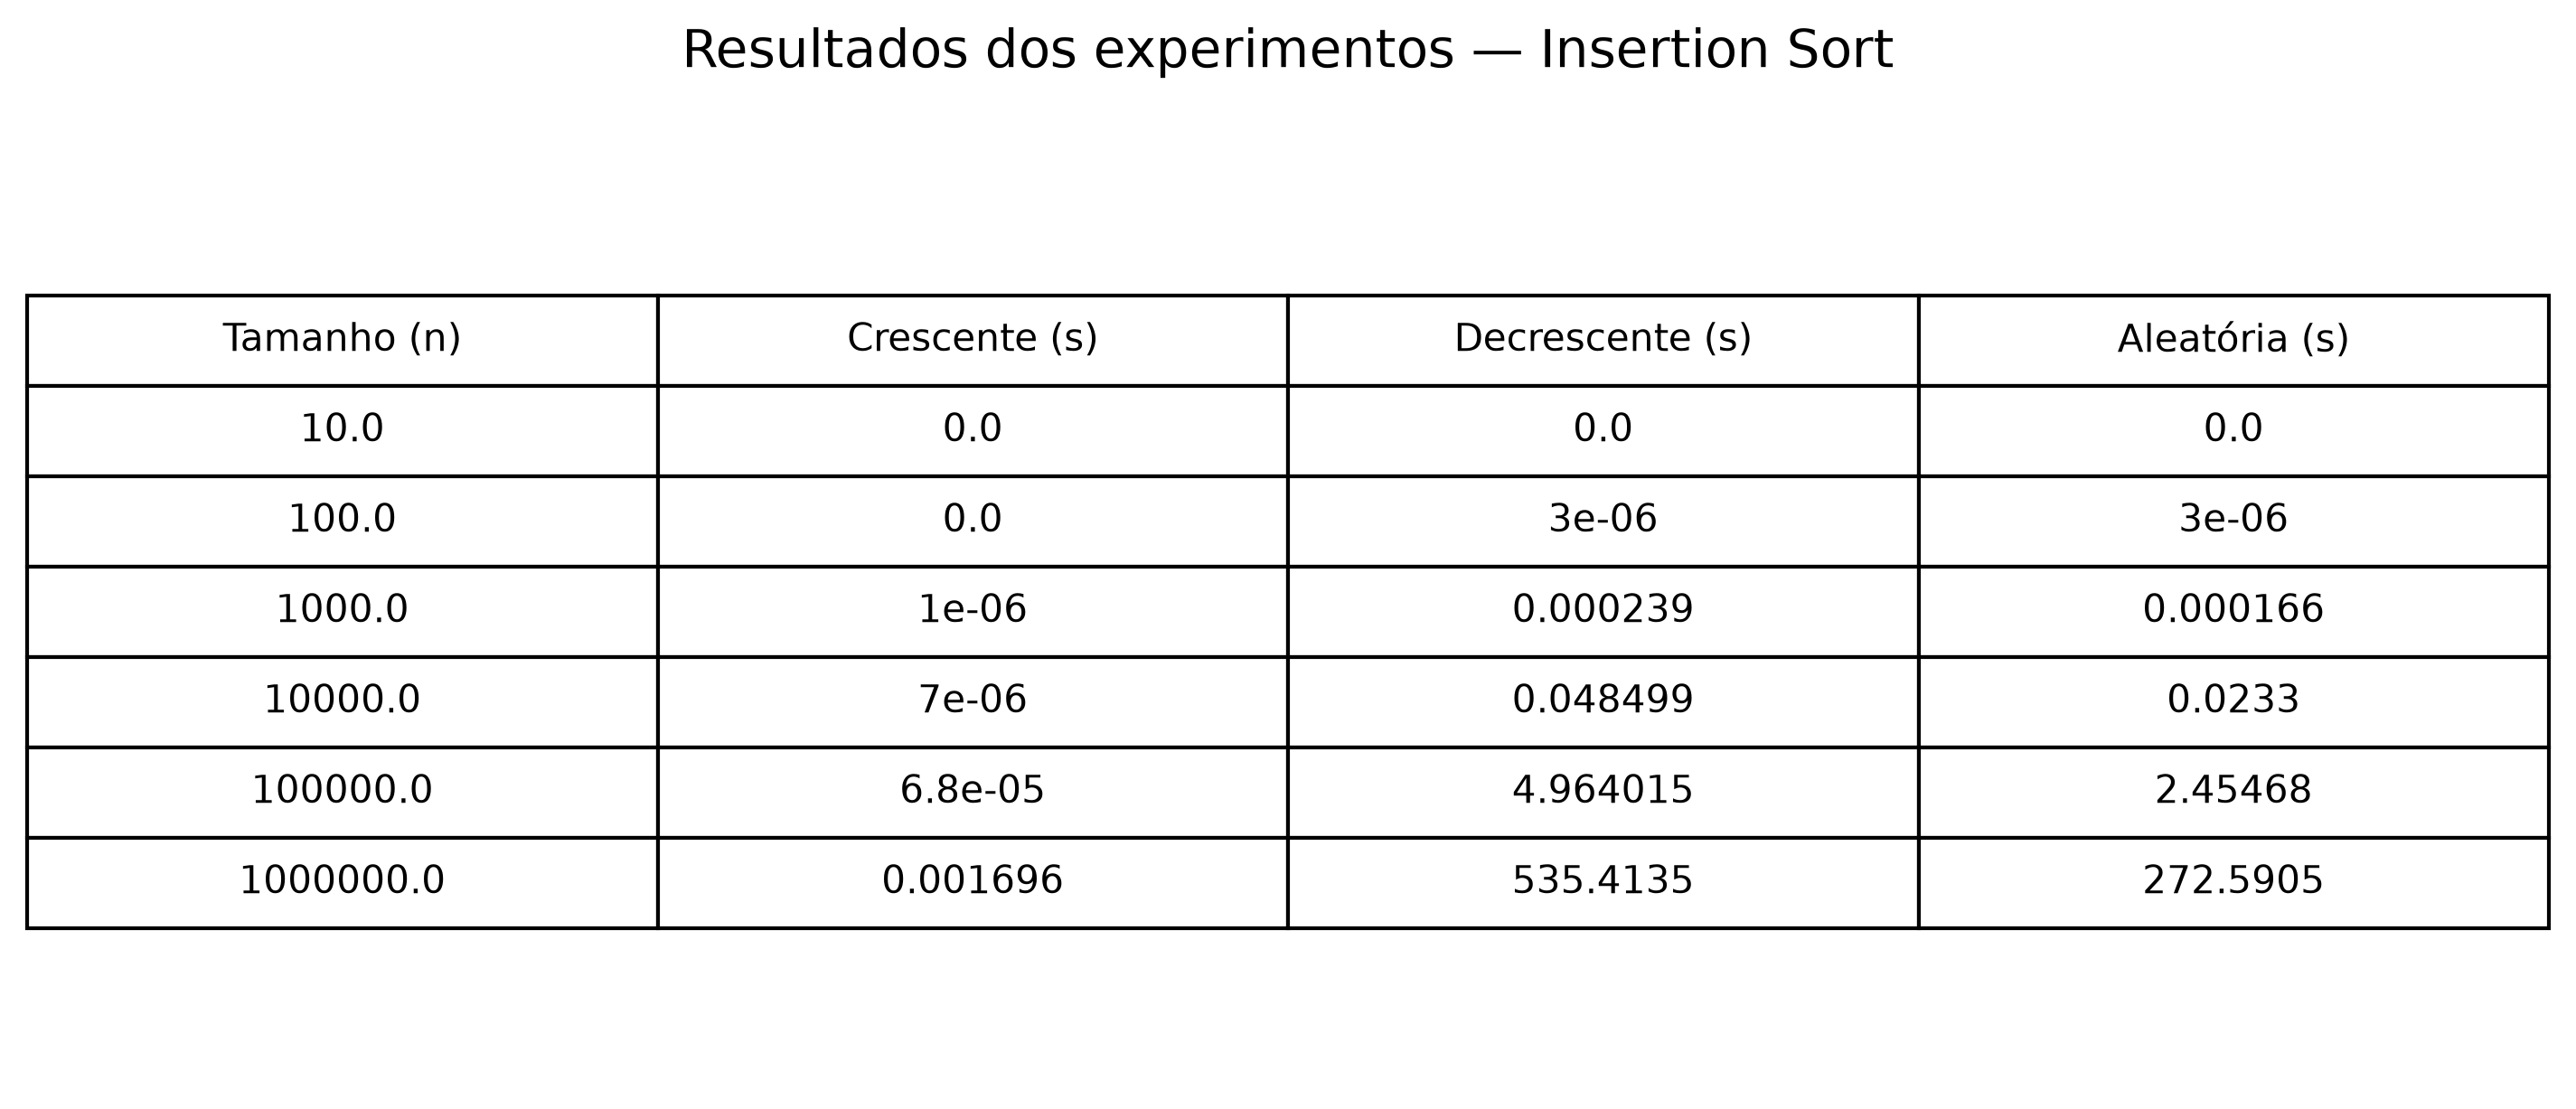
\includegraphics[width=16cm]{Imagens/Insertion_Sort/tabela.png}
    \caption{Tabela de tempo de execução do algoritmo Insertion Sort}
    \label{fig:tabela-insertion}
\end{figure}

\begin{figure}[H]
    \centering
    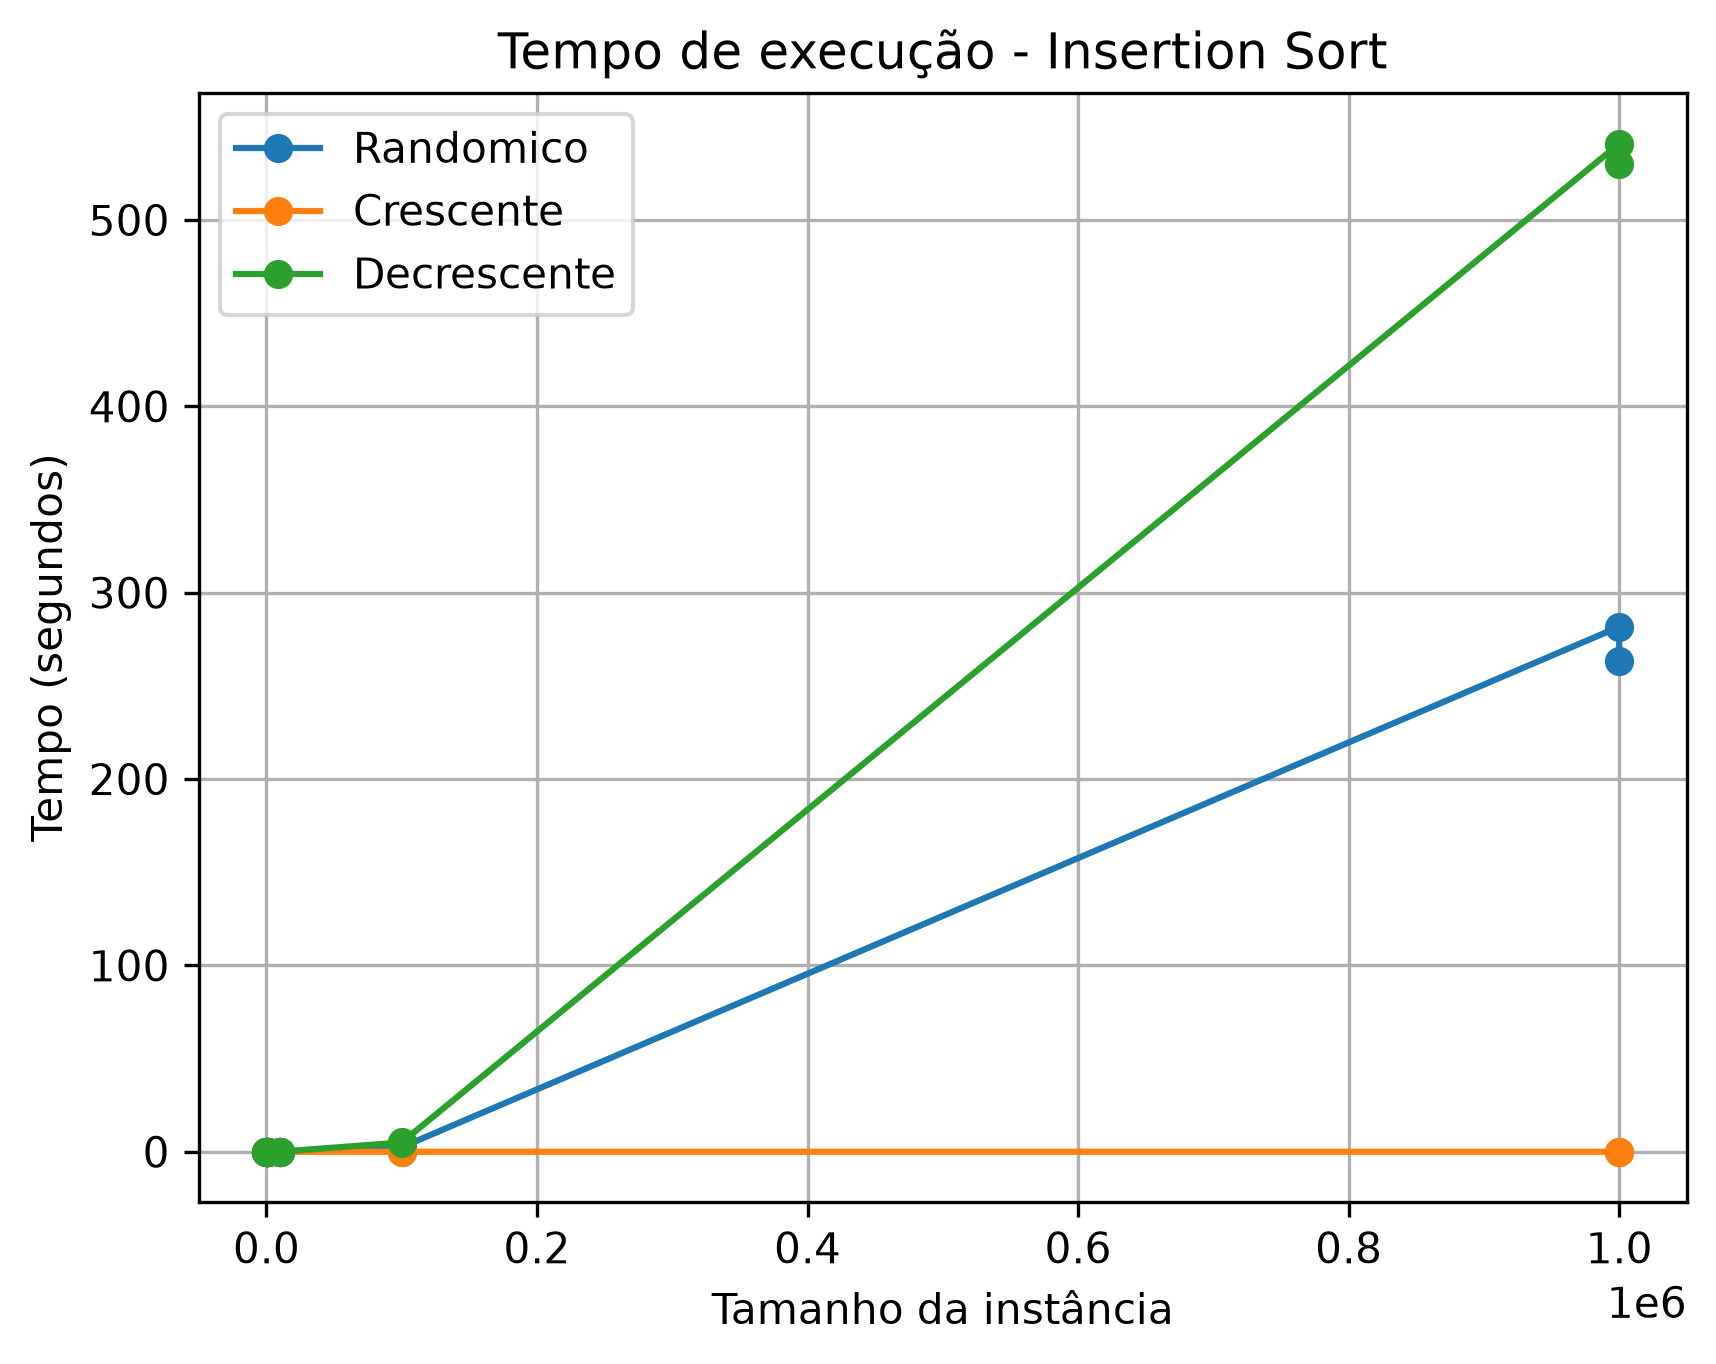
\includegraphics[width=10cm]{Imagens/Insertion_Sort/grafico.png}
    \caption{Gráfico de tempo de execução do algoritmo Insertion Sort}
    \label{fig:grafico-insertion}
\end{figure}

Os resultados obtidos nos experimentos estão apresentados na tabela e no
gráfico. Observa-se que o algoritmo Insertion Sort apresenta melhor
desempenho para instâncias ordenadas de forma crescente, uma vez que,
nesse caso, praticamente não são necessárias movimentações dos elementos.

Em contrapartida, as instâncias ordenadas de forma decrescente apresentam
os maiores tempos de execução. Isso ocorre porque cada novo elemento
precisa ser comparado e deslocado por uma grande quantidade de posições,
caracterizando o pior caso do algoritmo, cuja complexidade é
$\Theta(n^2)$.

As instâncias aleatórias apresentam desempenho intermediário, pois a
quantidade de deslocamentos depende da disposição inicial dos elementos.

A partir dos dados, também é possível perceber que o aumento do tamanho
da entrada provoca um crescimento significativo no tempo de execução,
principalmente nos casos aleatório e decrescente. Para a instância de
tamanho $n = 1.000.000$, o tempo registrado foi aproximadamente
$272{,}59$ segundos para a entrada aleatória e $535{,}41$ segundos para a
entrada decrescente. Já para a entrada crescente, o tempo foi de
aproximadamente $0{,}001696$ segundos.

Esses resultados confirmam o comportamento teórico esperado para o
algoritmo Insertion Sort.

\subsection{Bubble Sort}
\begin{figure}[H]
\centering
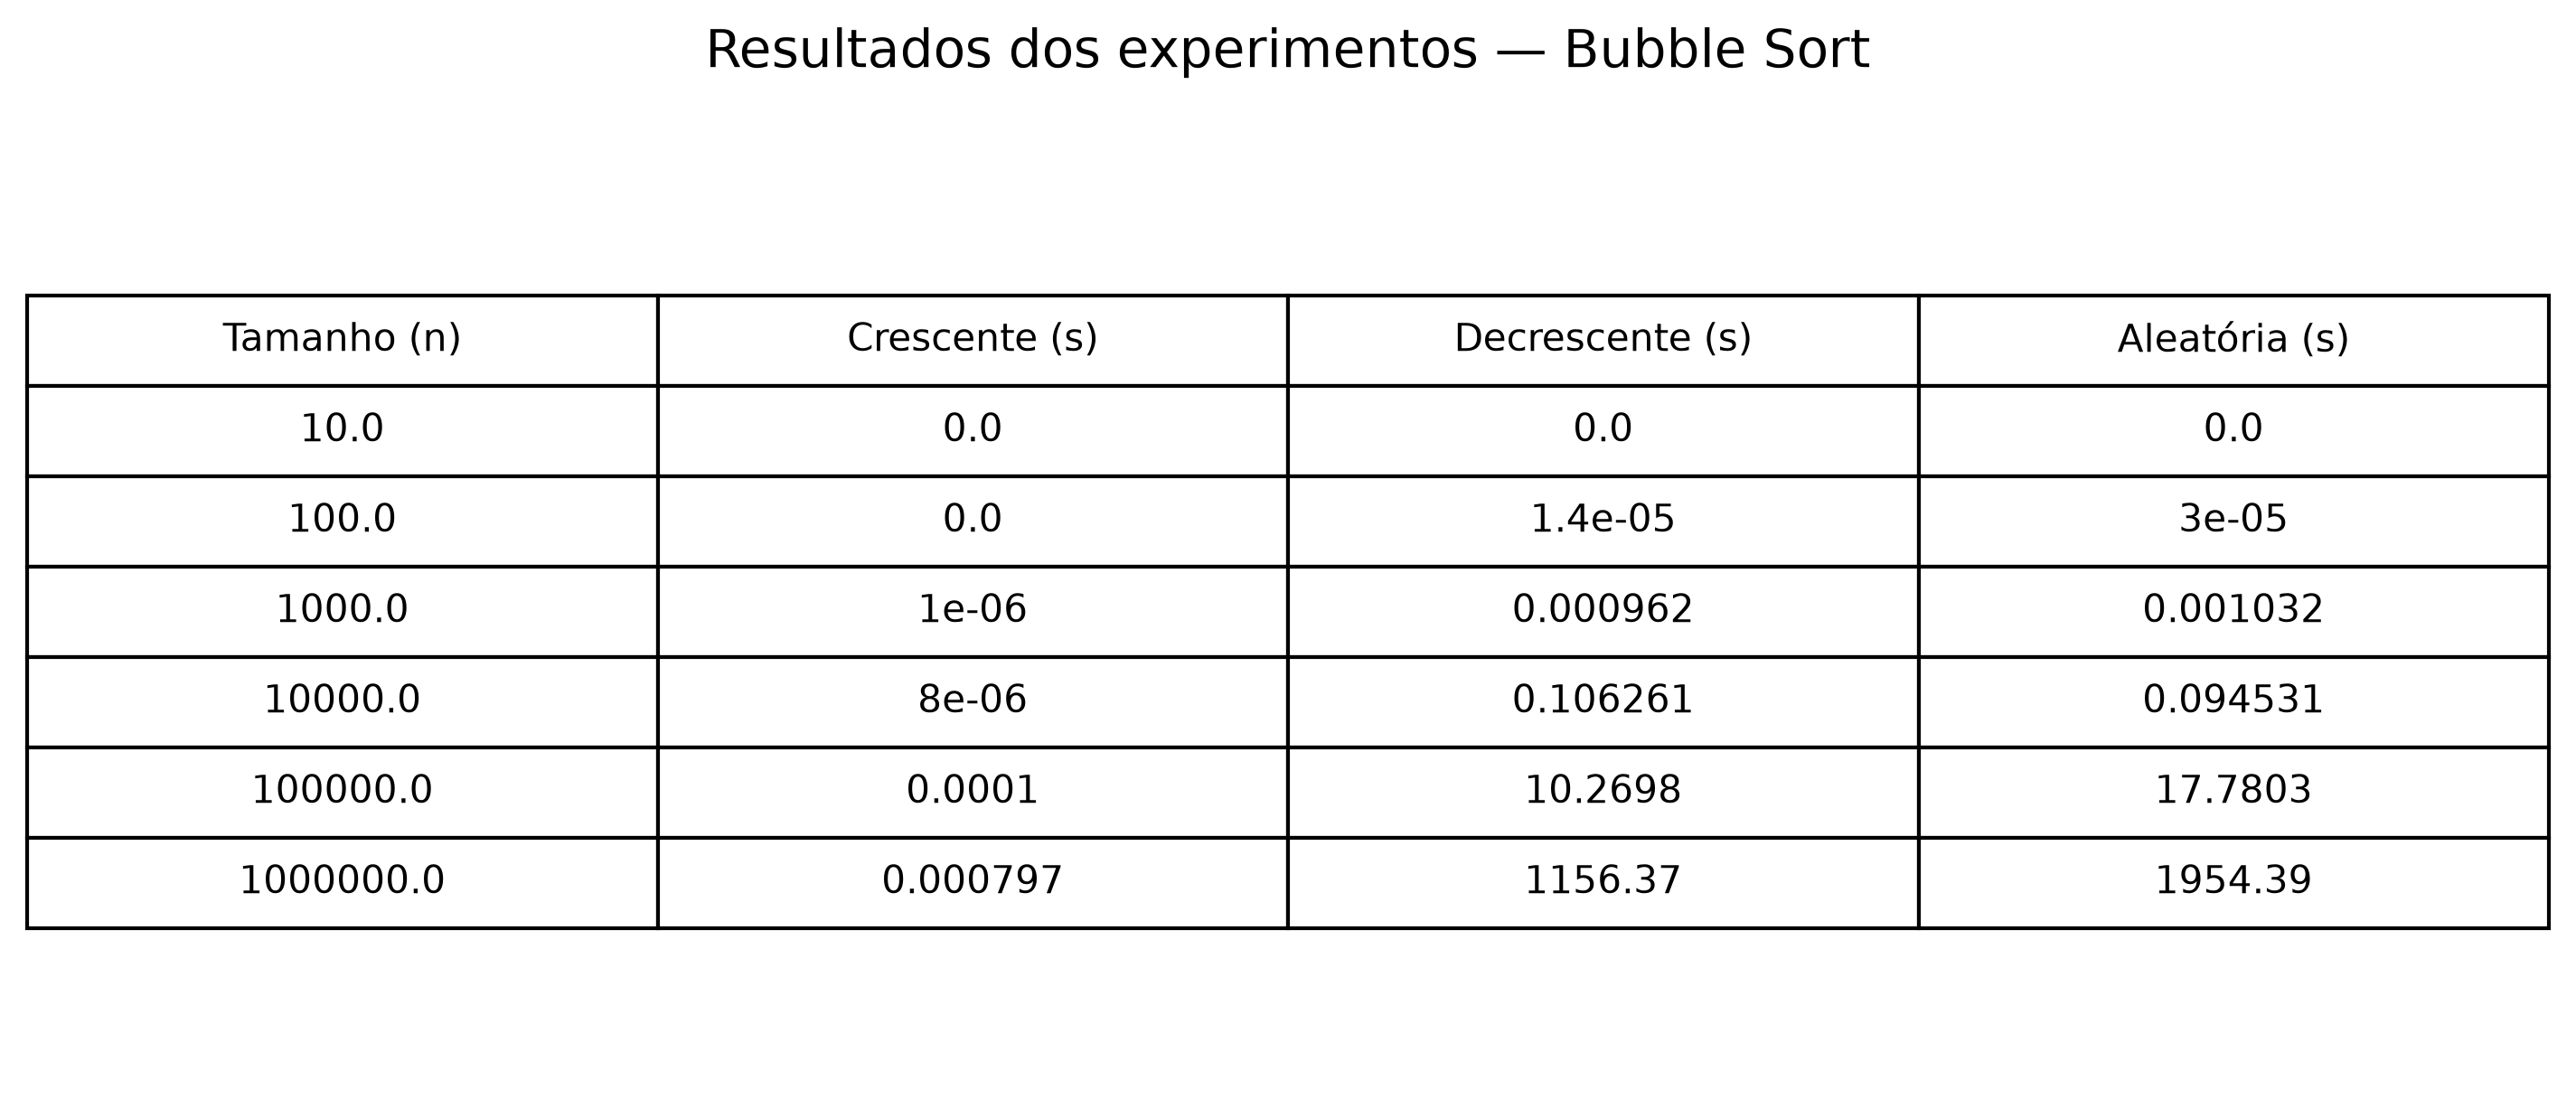
\includegraphics[width=16cm]{Imagens/Bubble_Sort/tabela.png}
\caption{Tabela de tempo de execução do algoritmo Bubble Sort}
\label{fig:tabela-bubble}
\end{figure}

\begin{figure}[H]
\centering
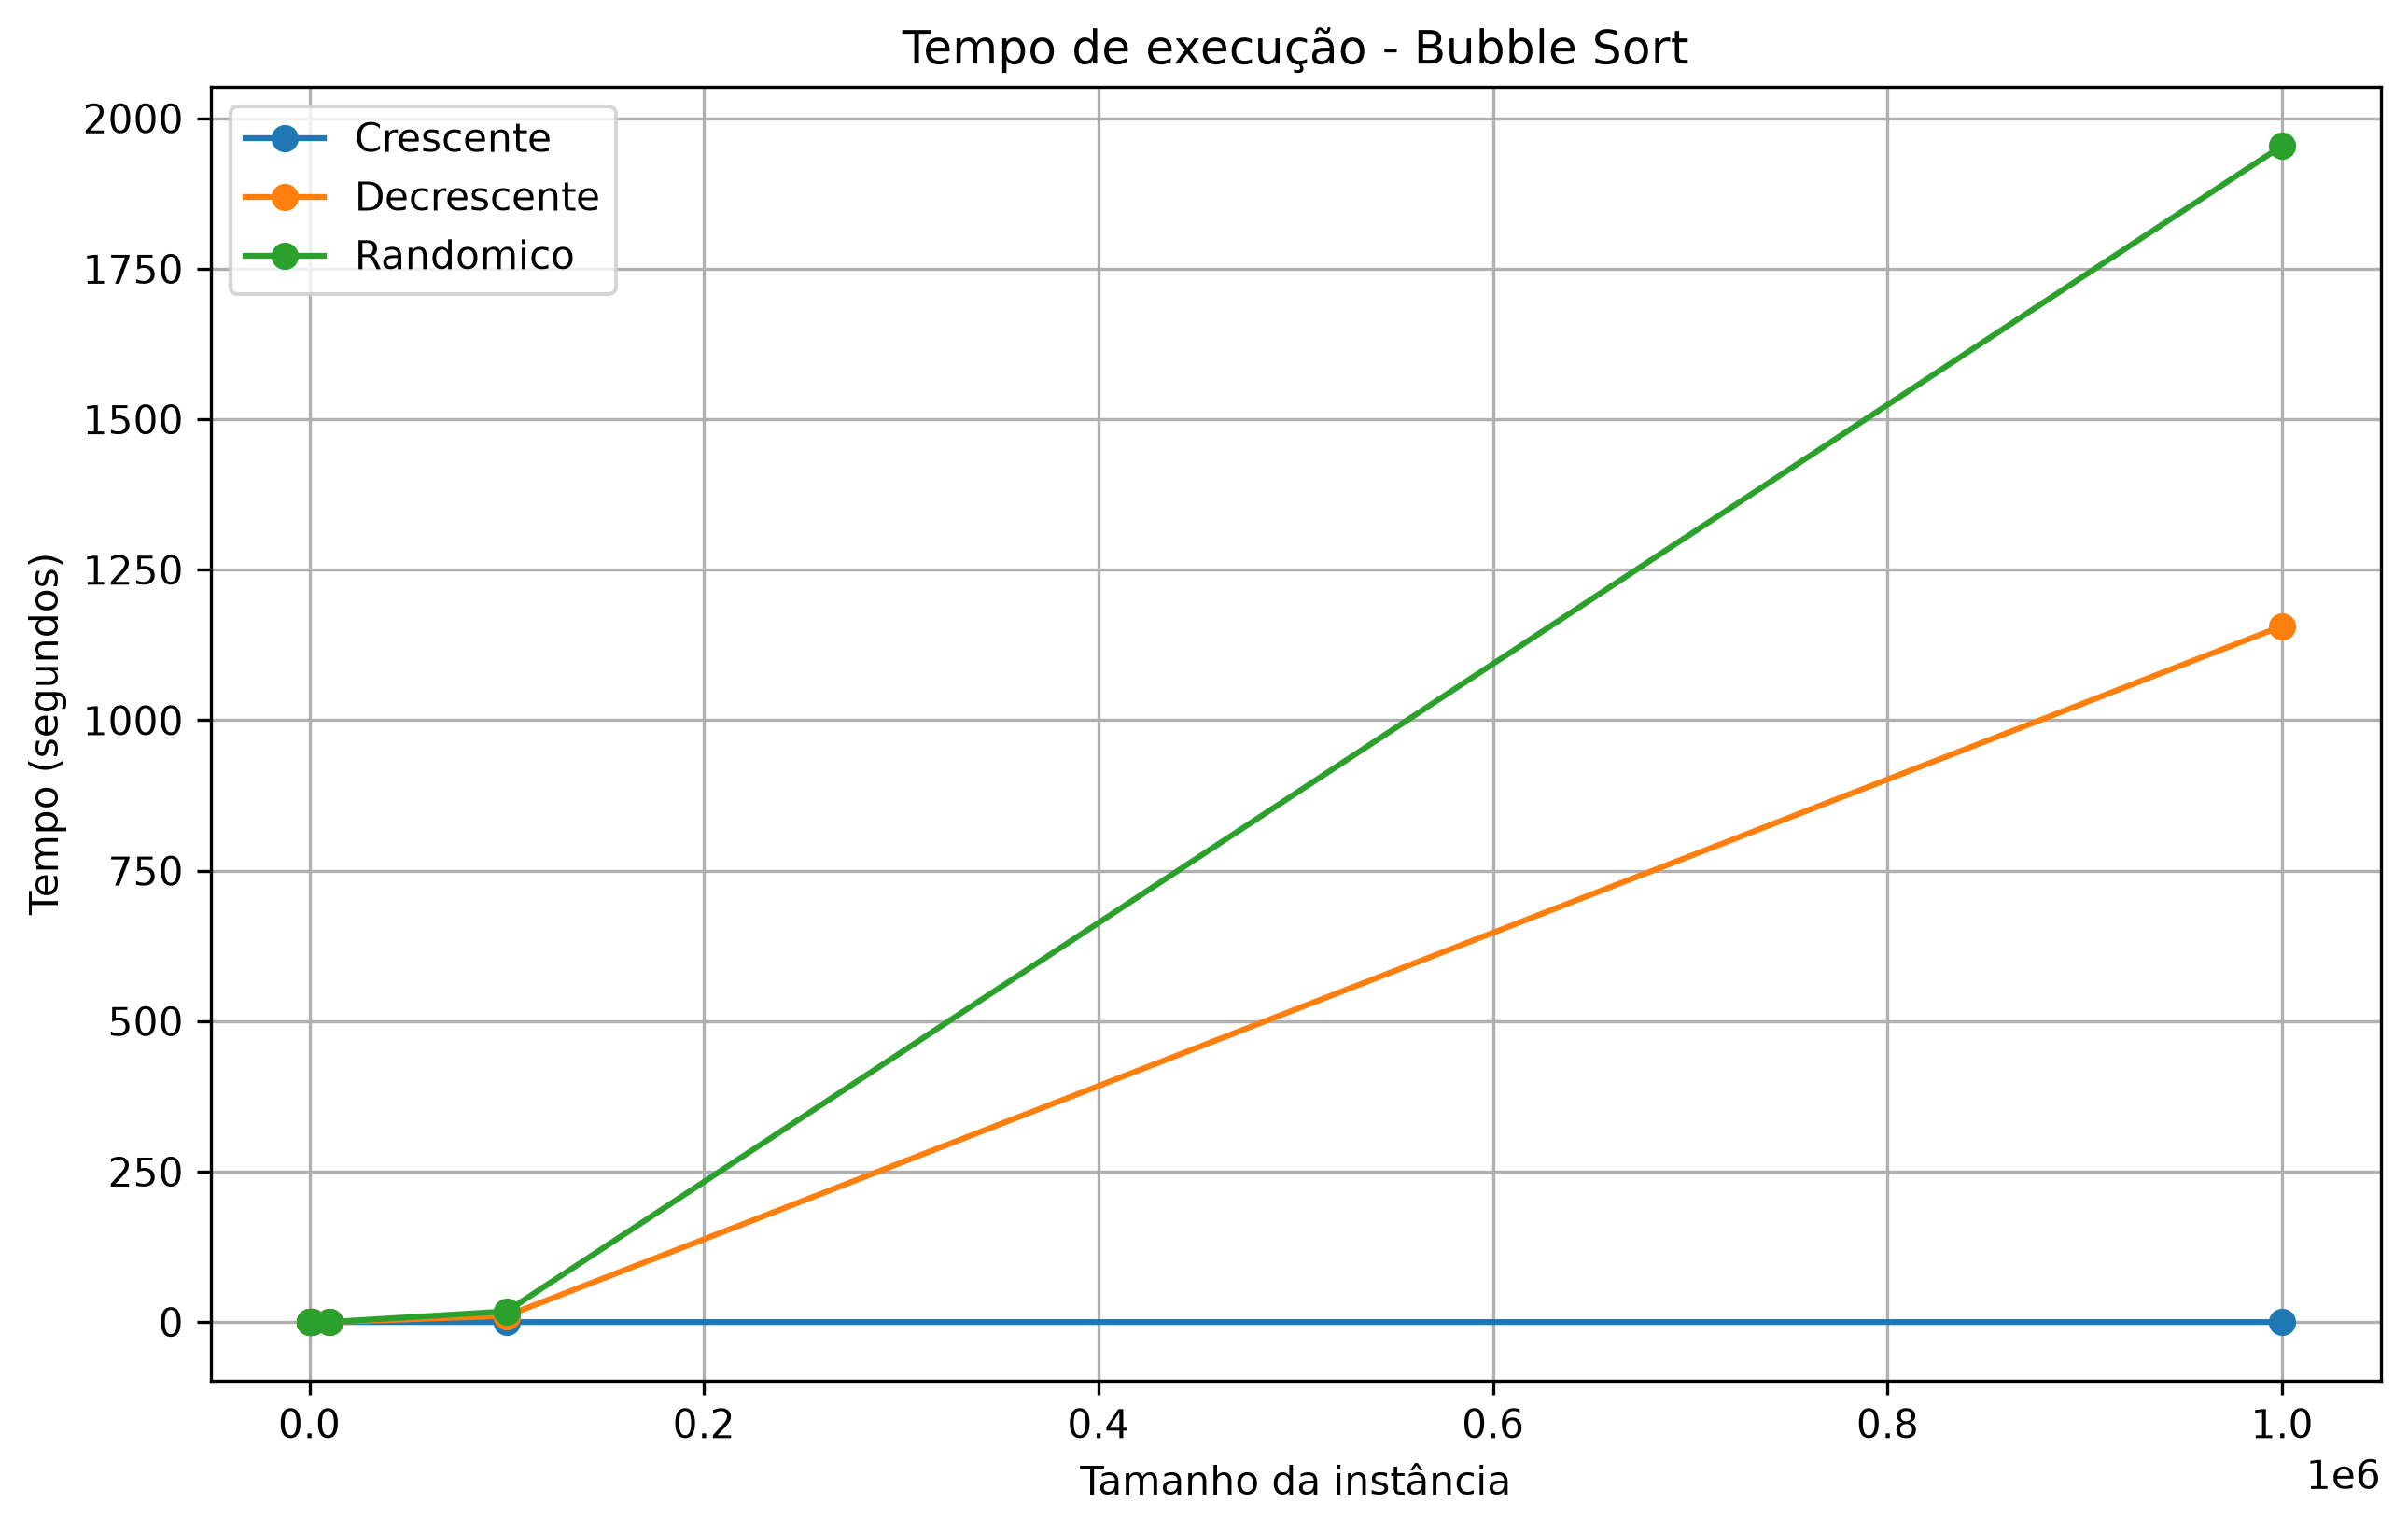
\includegraphics[width=10cm]{Imagens/Bubble_Sort/grafico.png}
\caption{Gráfico de tempo de execução do algoritmo Bubble Sort}
\label{fig:grafico-bubble}
\end{figure}

Os resultados obtidos nos experimentos estão apresentados na tabela e no
gráfico. Observa-se que o algoritmo Bubble Sort apresenta comportamentos
diferentes de acordo com a organização inicial dos elementos, devido à
utilização da variável \texttt{trocou}, que permite interromper a execução
quando nenhuma troca é realizada durante uma passagem.

Nas instâncias ordenadas de forma crescente, nenhuma troca é realizada
durante a primeira passagem. Dessa forma, a variável \texttt{trocou}
permanece com valor \texttt{false} e o algoritmo encerra sua execução por
meio do comando \texttt{break}, fazendo com que o melhor caso apresente
complexidade $\Theta(n)$.

Nas instâncias ordenadas de forma decrescente, além das comparações,
também são necessárias diversas trocas para colocar os elementos em suas
posições corretas. Como ocorre pelo menos uma troca durante cada passagem,
o comando \texttt{break} não é executado antes do término das passagens
previstas, caracterizando o pior caso do algoritmo, cuja complexidade é
$\Theta(n^2)$.

As instâncias aleatórias apresentam uma quantidade intermediária de
trocas, pois o número de elementos que precisam ser deslocados depende da
organização inicial do vetor. Entretanto, o algoritmo normalmente realiza
diversas passagens pelo vetor, fazendo com que o caso médio apresente
complexidade $\Theta(n^2)$.

A partir dos dados, também é possível perceber que o aumento do tamanho
da entrada provoca um crescimento significativo no tempo de execução,
principalmente nas entradas aleatórias e decrescentes. Nas entradas
crescentes, o algoritmo pode encerrar a execução após a primeira passagem,
devido à ausência de trocas.

Esses resultados apresentam comportamento compatível com a análise de
complexidade do algoritmo Bubble Sort, considerando a otimização utilizada
na implementação por meio da variável \texttt{trocou}.


\subsection{Selection Sort}
\begin{figure}[H]
\centering
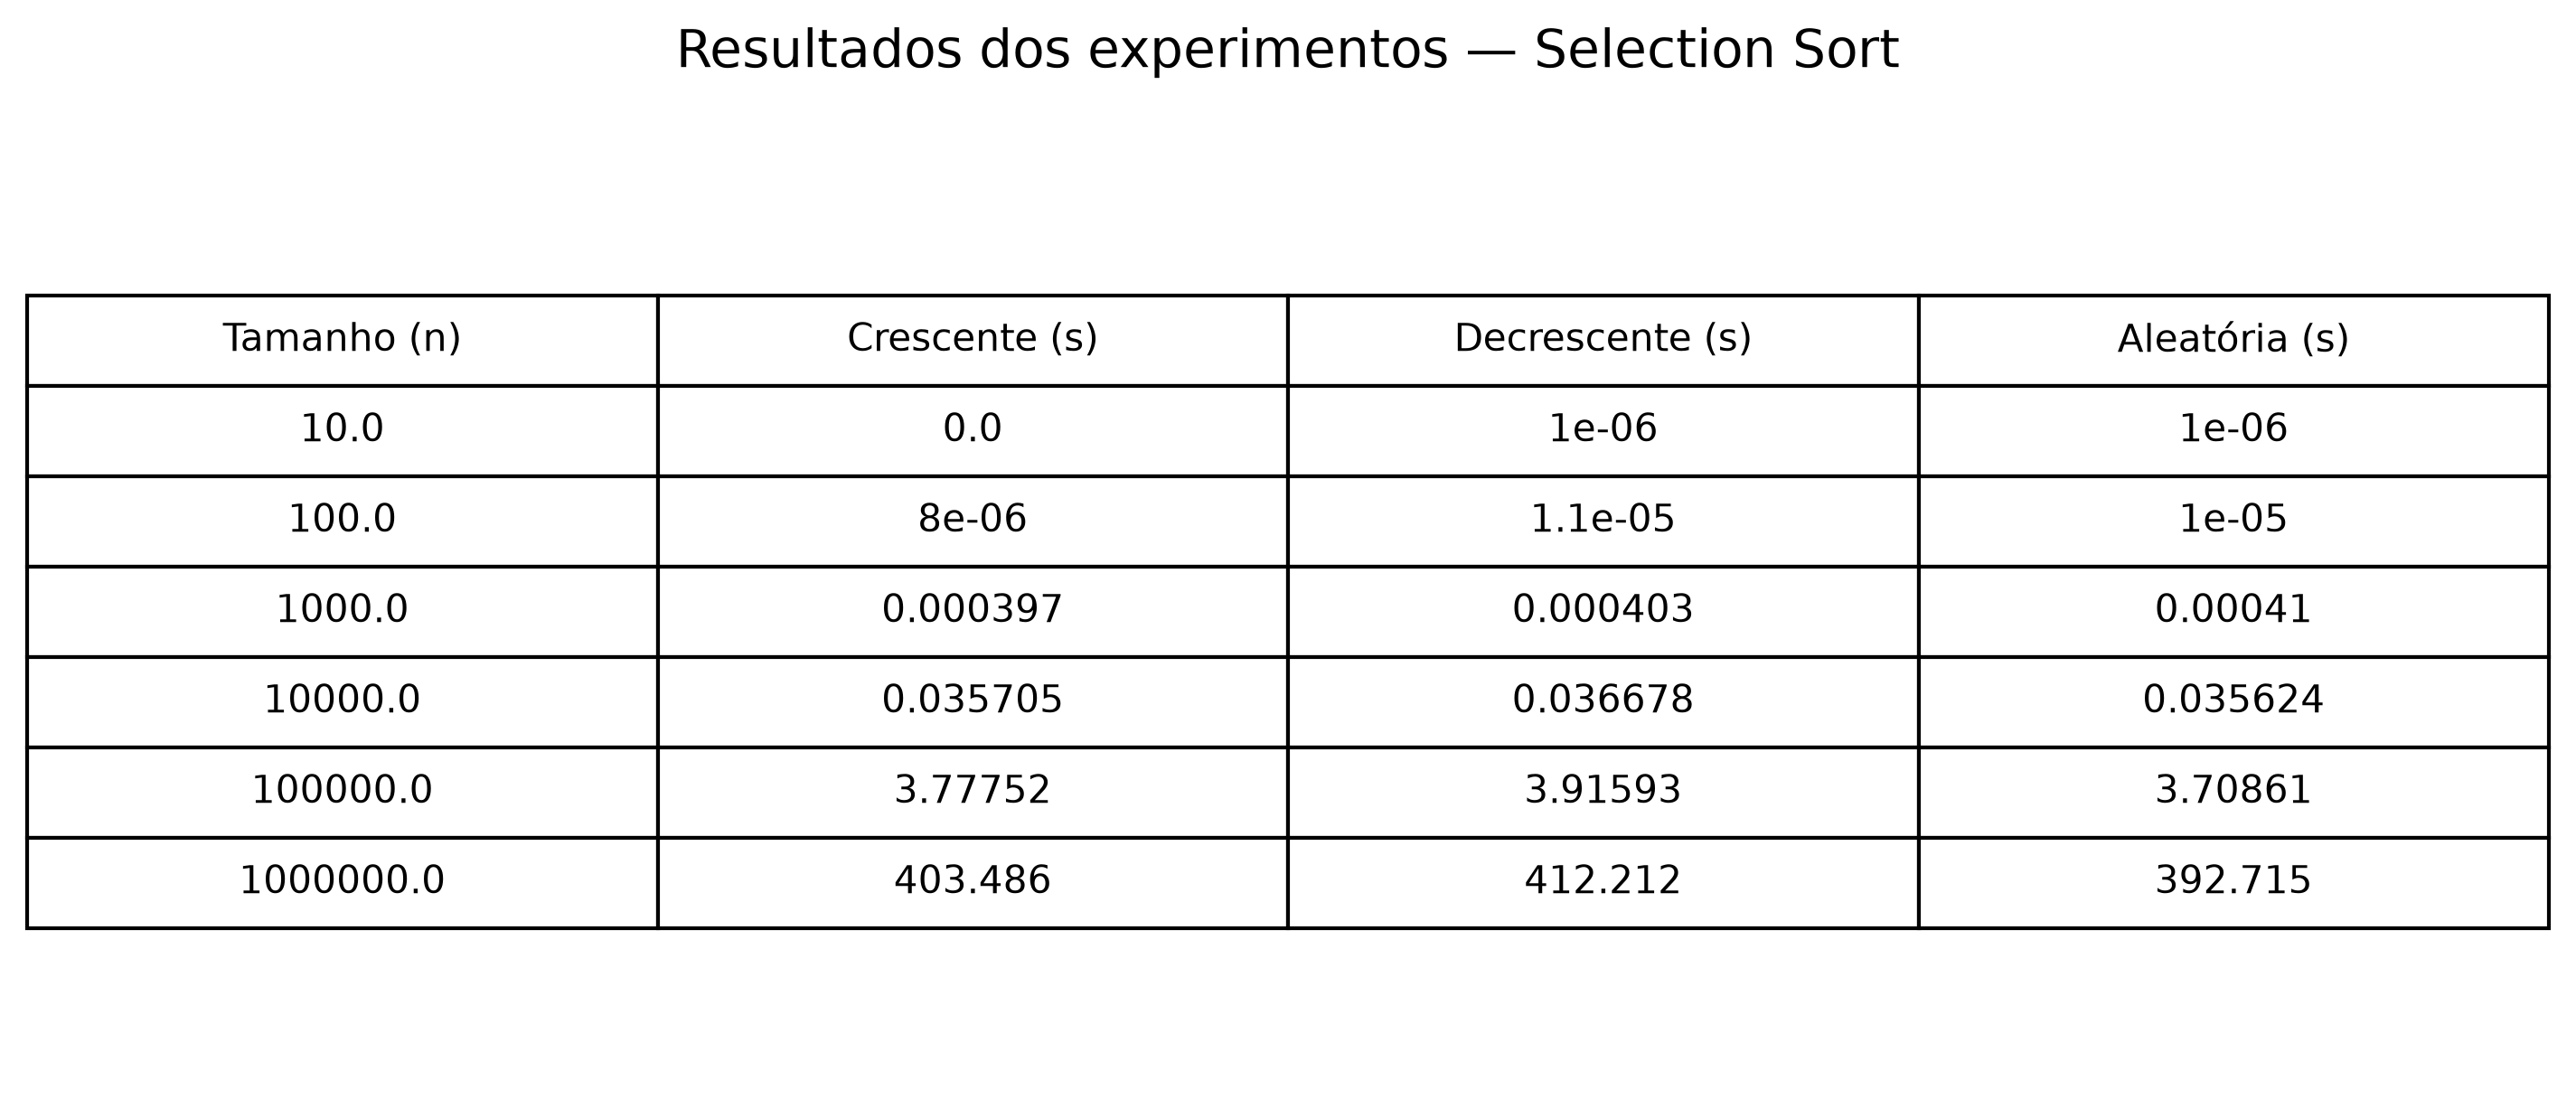
\includegraphics[width=16cm]{Imagens/Selection_Sort/tabela.png}
\caption{Tabela de tempo de execução do algoritmo Selection Sort}
\label{fig:tabela-selection}
\end{figure}

\begin{figure}[H]
\centering
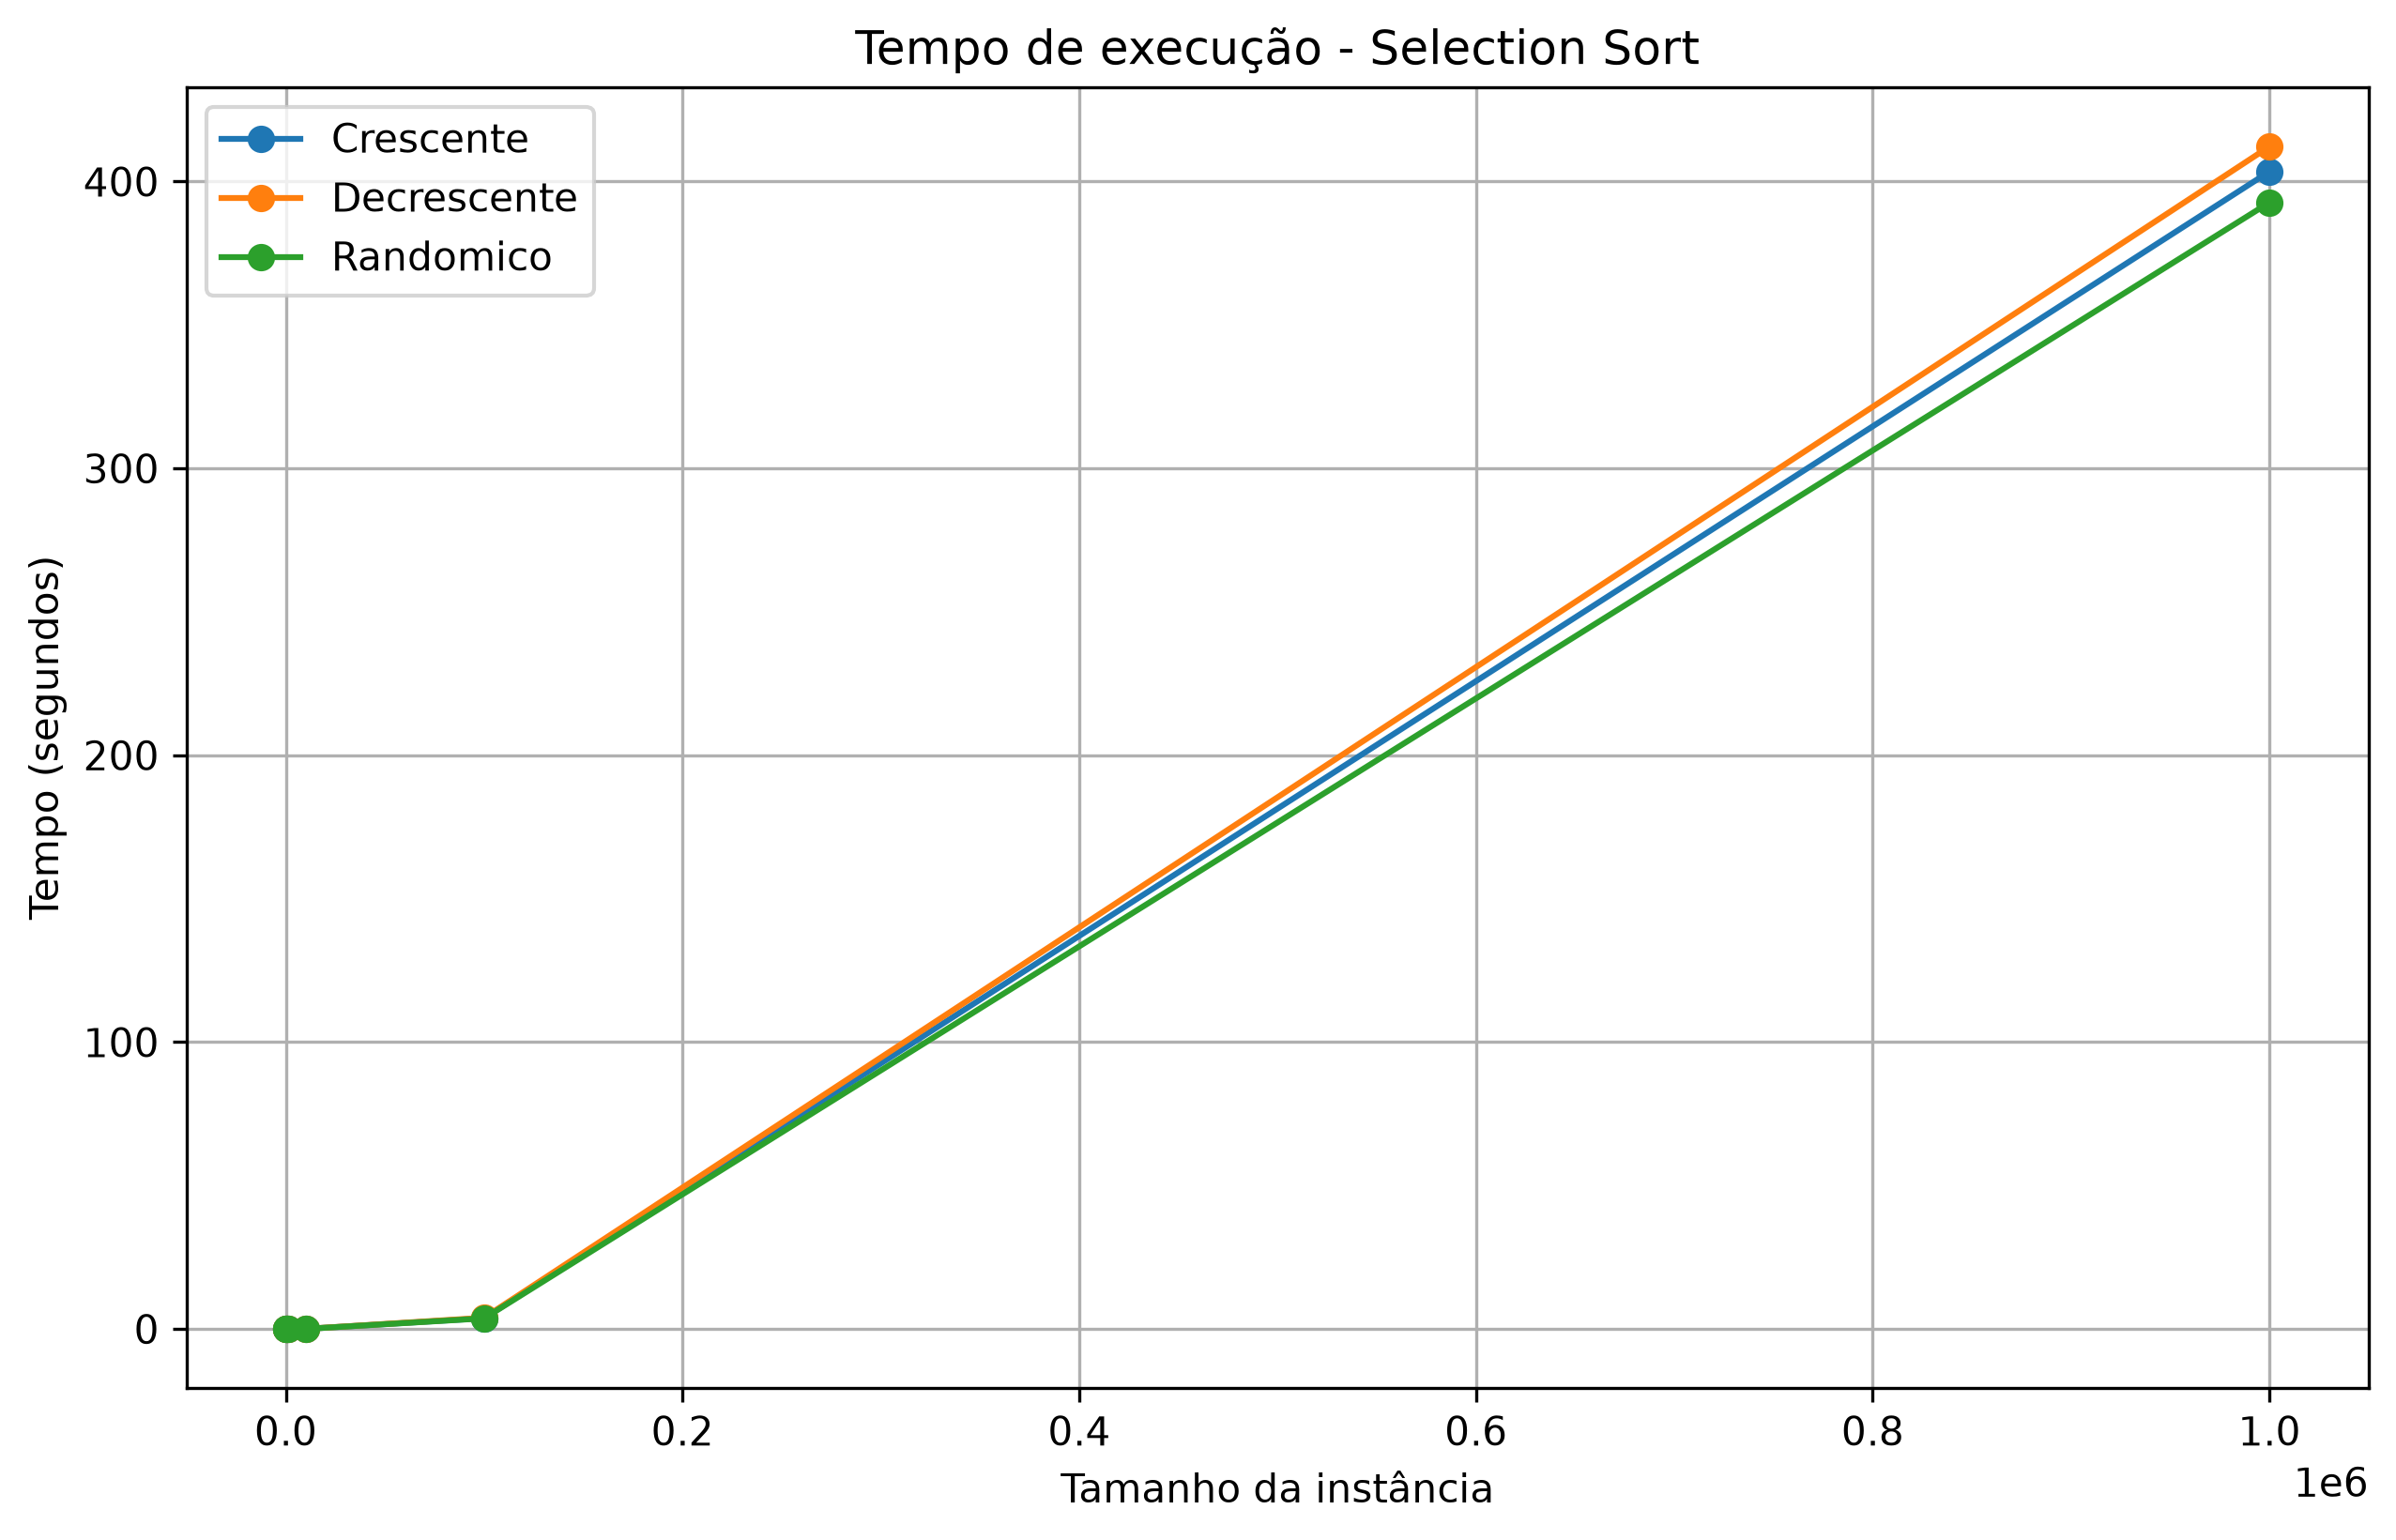
\includegraphics[width=10cm]{Imagens/Selection_Sort/grafico.png}
\caption{Gráfico de tempo de execução do algoritmo Selection Sort}
\label{fig:grafico-selection}
\end{figure}

Os resultados obtidos nos experimentos estão apresentados na tabela e no
gráfico. Observa-se que o algoritmo Selection Sort apresenta comportamento
semelhante nos diferentes tipos de entrada, pois a quantidade de
comparações realizadas não depende da organização inicial dos elementos.

Nas instâncias ordenadas de forma crescente, o algoritmo ainda precisa
percorrer a parte não ordenada do vetor para encontrar o menor elemento.
Dessa forma, mesmo quando os elementos já estão organizados, são
realizadas aproximadamente as mesmas comparações previstas para os demais
tipos de entrada.

Nas instâncias ordenadas de forma decrescente, o algoritmo também realiza
a mesma quantidade de comparações, embora a posição do menor elemento
encontrado possa exigir mais trocas para colocá-lo na posição correta.

As instâncias aleatórias apresentam comportamento semelhante, pois,
independentemente da disposição inicial dos elementos, o algoritmo
continua procurando o menor elemento em toda a parte ainda não ordenada
do vetor.

A partir dos dados, também é possível perceber que o aumento do tamanho
da entrada provoca um crescimento significativo no tempo de execução.
Esse comportamento está de acordo com a análise teórica, segundo a qual
o Selection Sort apresenta complexidade $\Theta(n^2)$ no melhor caso,
caso médio e pior caso.

Assim, os resultados experimentais apresentam comportamento compatível
com a análise de complexidade do algoritmo Selection Sort.


\subsection{Shell Sort}
\begin{figure}[H]
\centering
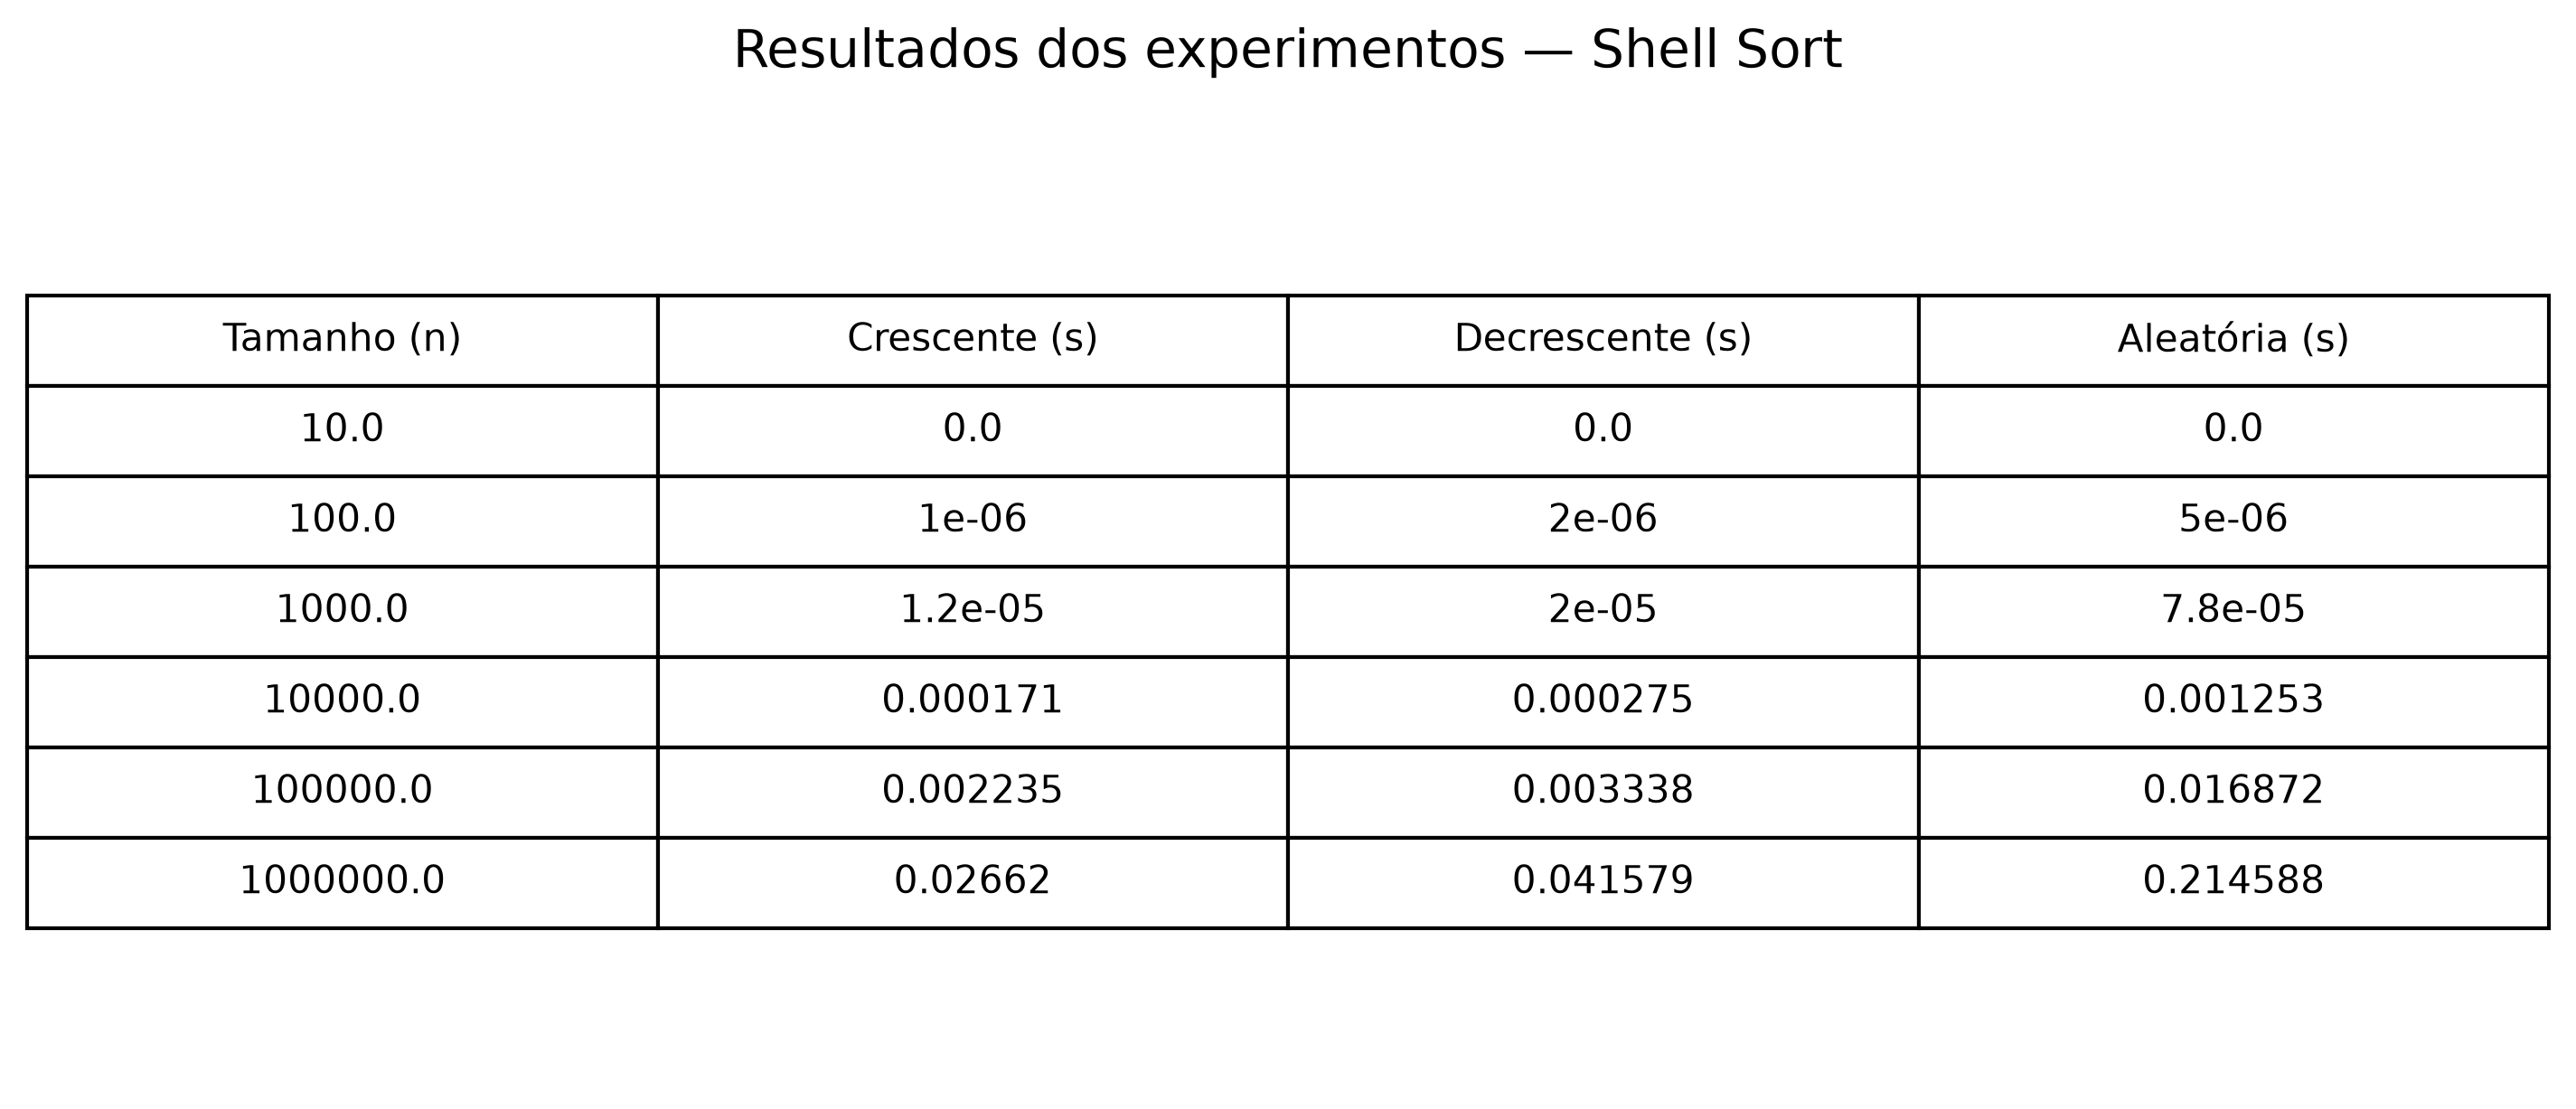
\includegraphics[width=16cm]{Imagens/Shell_Sort/tabela.png}
\caption{Tabela de tempo de execução do algoritmo Shell Sort}
\label{fig:tabela-shell}
\end{figure}

\begin{figure}[H]
\centering
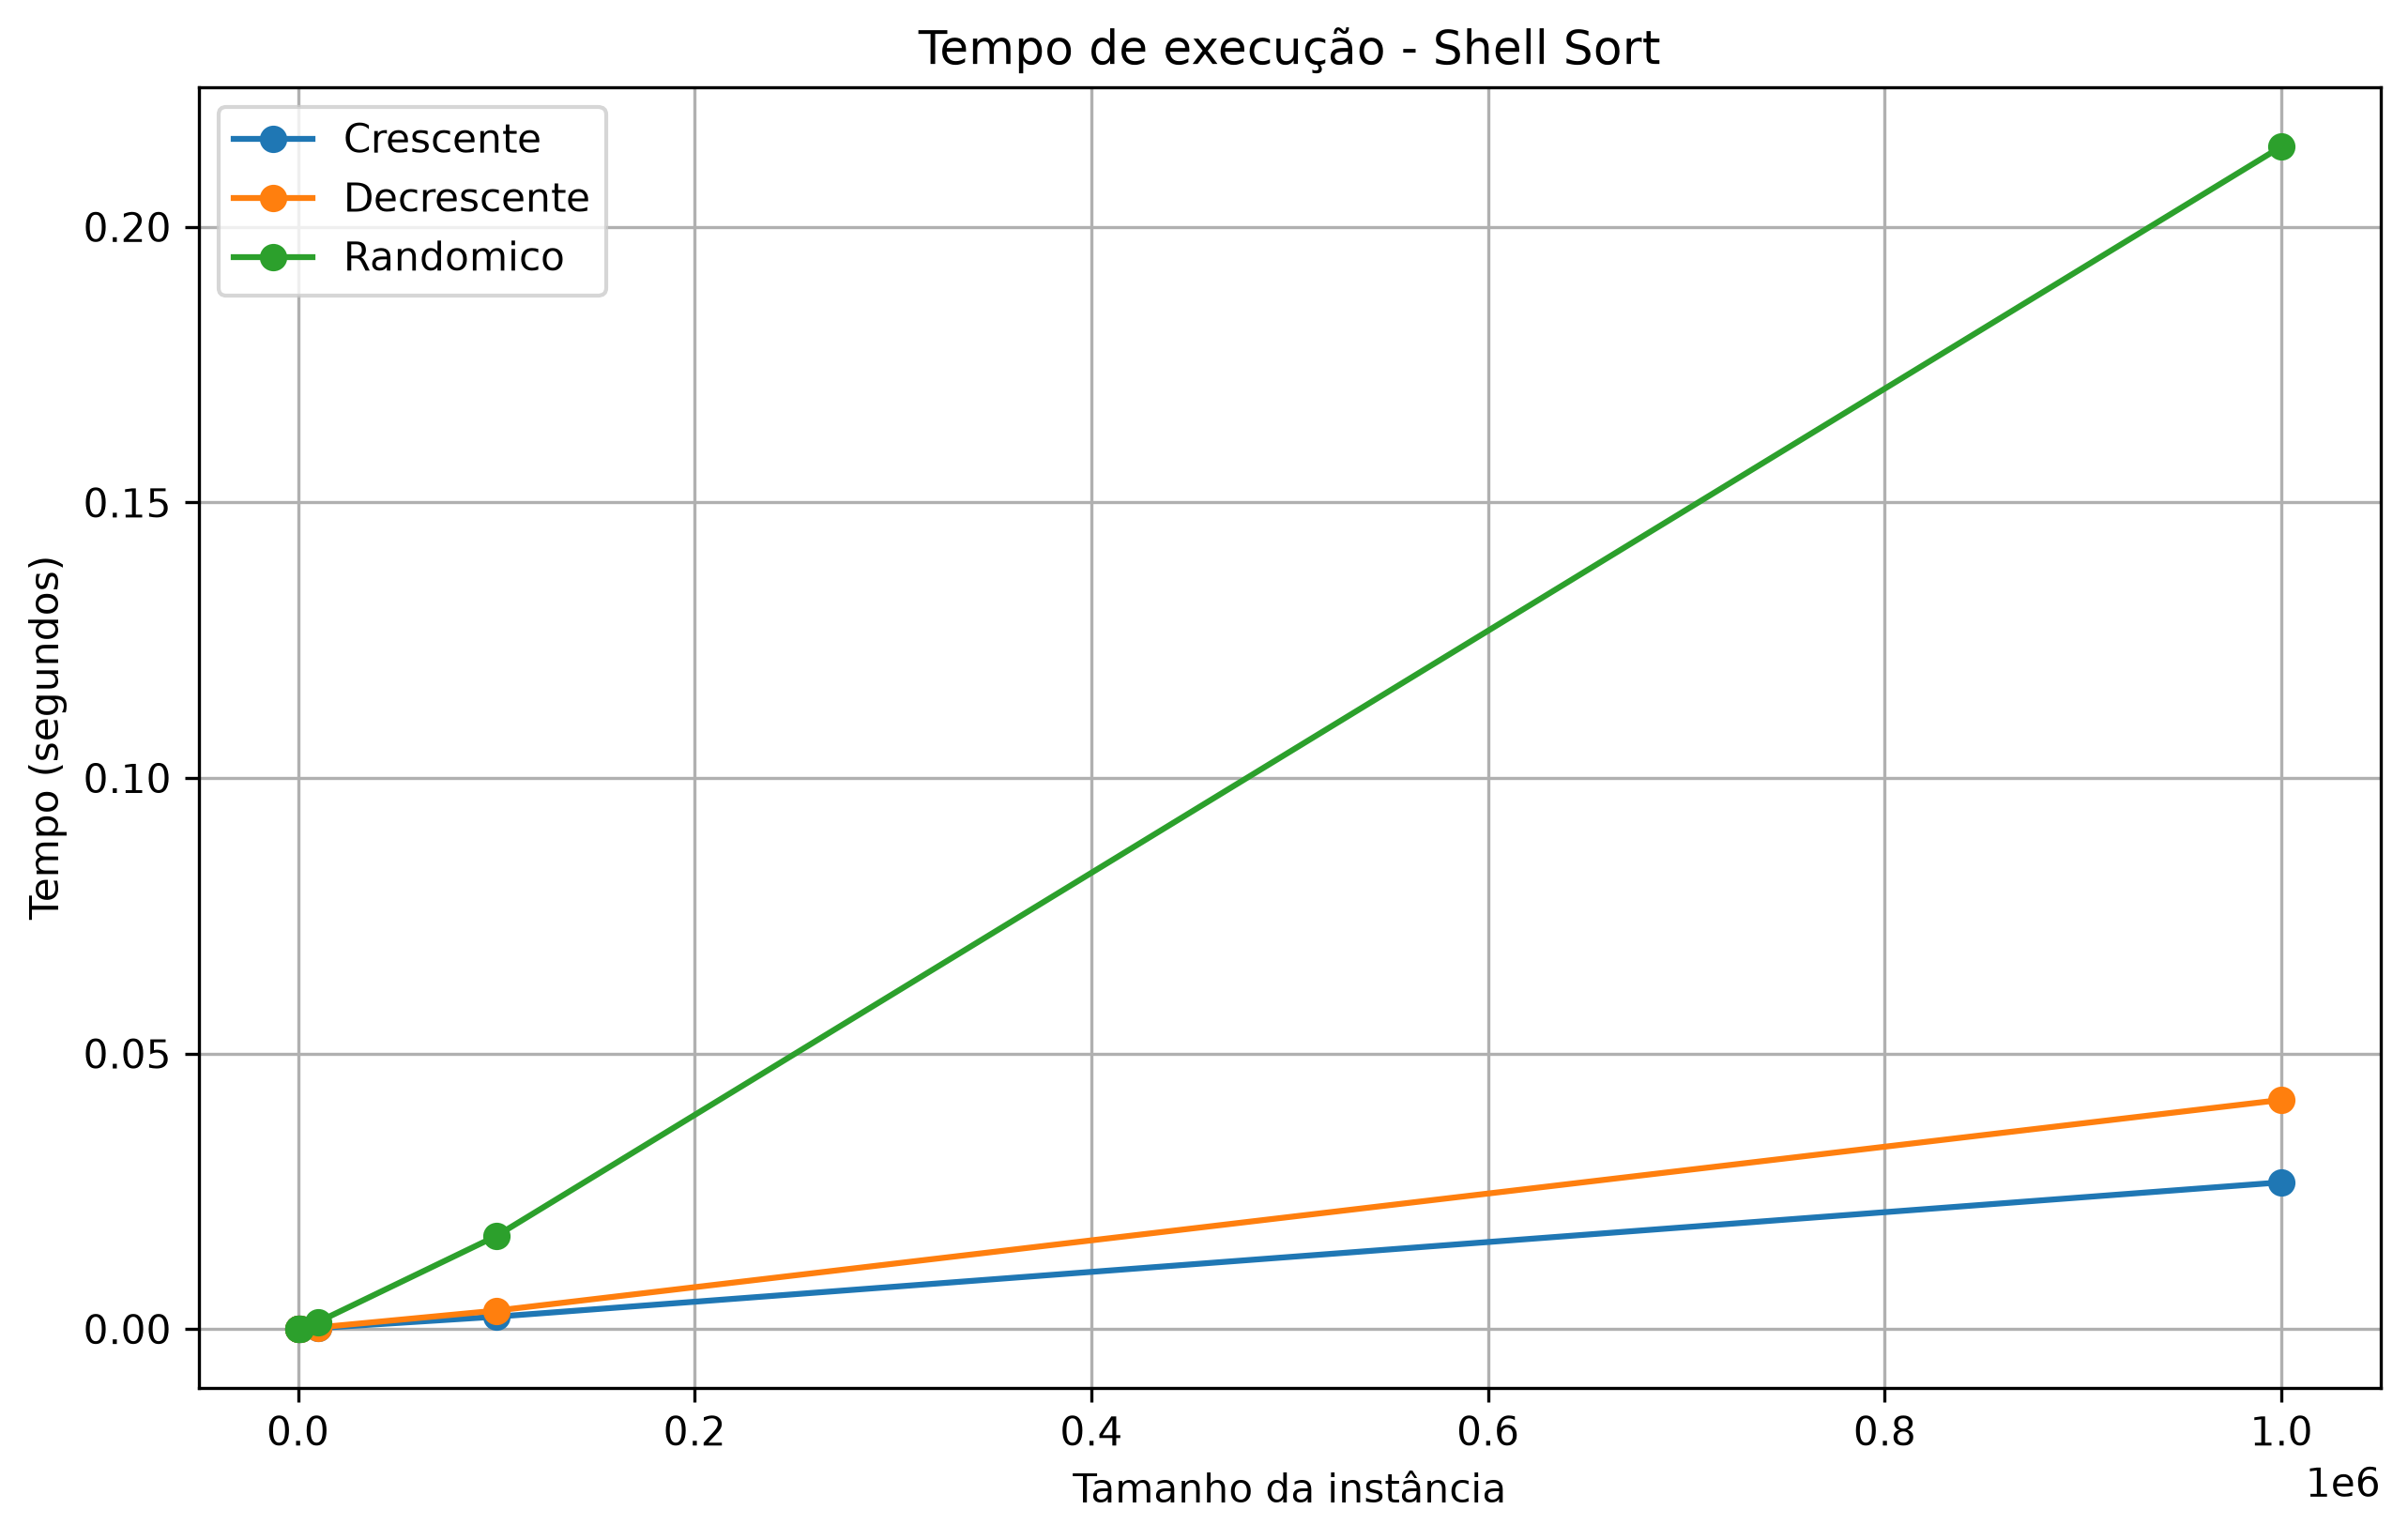
\includegraphics[width=10cm]{Imagens/Shell_Sort/grafico.png}
\caption{Gráfico de tempo de execução do algoritmo Shell Sort}
\label{fig:grafico-shell}
\end{figure}

Os resultados obtidos nos experimentos estão apresentados na tabela e no
gráfico. O algoritmo Shell Sort apresenta um comportamento diferente dos
demais algoritmos analisados, pois seu desempenho é influenciado pela
sequência de \textit{gaps} utilizada. Nos experimentos deste trabalho,
foi utilizado o divisor 2, produzindo uma sequência de \textit{gaps}
obtida pela divisão sucessiva do tamanho da entrada por 2 até atingir o
valor 1.

Nas instâncias ordenadas de forma crescente, os elementos já se encontram
em suas posições relativas para os diferentes \textit{gaps}, reduzindo a
quantidade de deslocamentos necessários durante a execução.

Nas instâncias ordenadas de forma decrescente, são necessários mais
deslocamentos para reorganizar os elementos. Entretanto, os
\textit{gaps} maiores permitem que elementos que estão distantes sejam
movimentados antes da etapa final, reduzindo parte da desordem do vetor.

As instâncias aleatórias apresentam comportamento intermediário, pois a
quantidade de comparações e deslocamentos depende da disposição inicial
dos elementos. O uso dos diferentes \textit{gaps} permite realizar
movimentações entre elementos distantes antes da ordenação final com
\textit{gap} igual a 1.

A partir dos dados, também é possível observar a influência do aumento do
tamanho da entrada no tempo de execução. O crescimento observado pode ser
relacionado à análise teórica do algoritmo, que depende da sequência de
\textit{gaps} utilizada. Para a sequência adotada neste trabalho, o pior
caso apresenta comportamento de ordem $\Theta(n^2)$, enquanto o melhor
caso apresenta comportamento de ordem $\Theta(n\log n)$.

Os resultados experimentais permitem, portanto, relacionar o
comportamento observado na tabela e no gráfico com a estratégia utilizada
pelo Shell Sort e com a influência da sequência de \textit{gaps} em seu
desempenho.


\subsection{Merge Sort}
\begin{figure}[H]
    \centering
    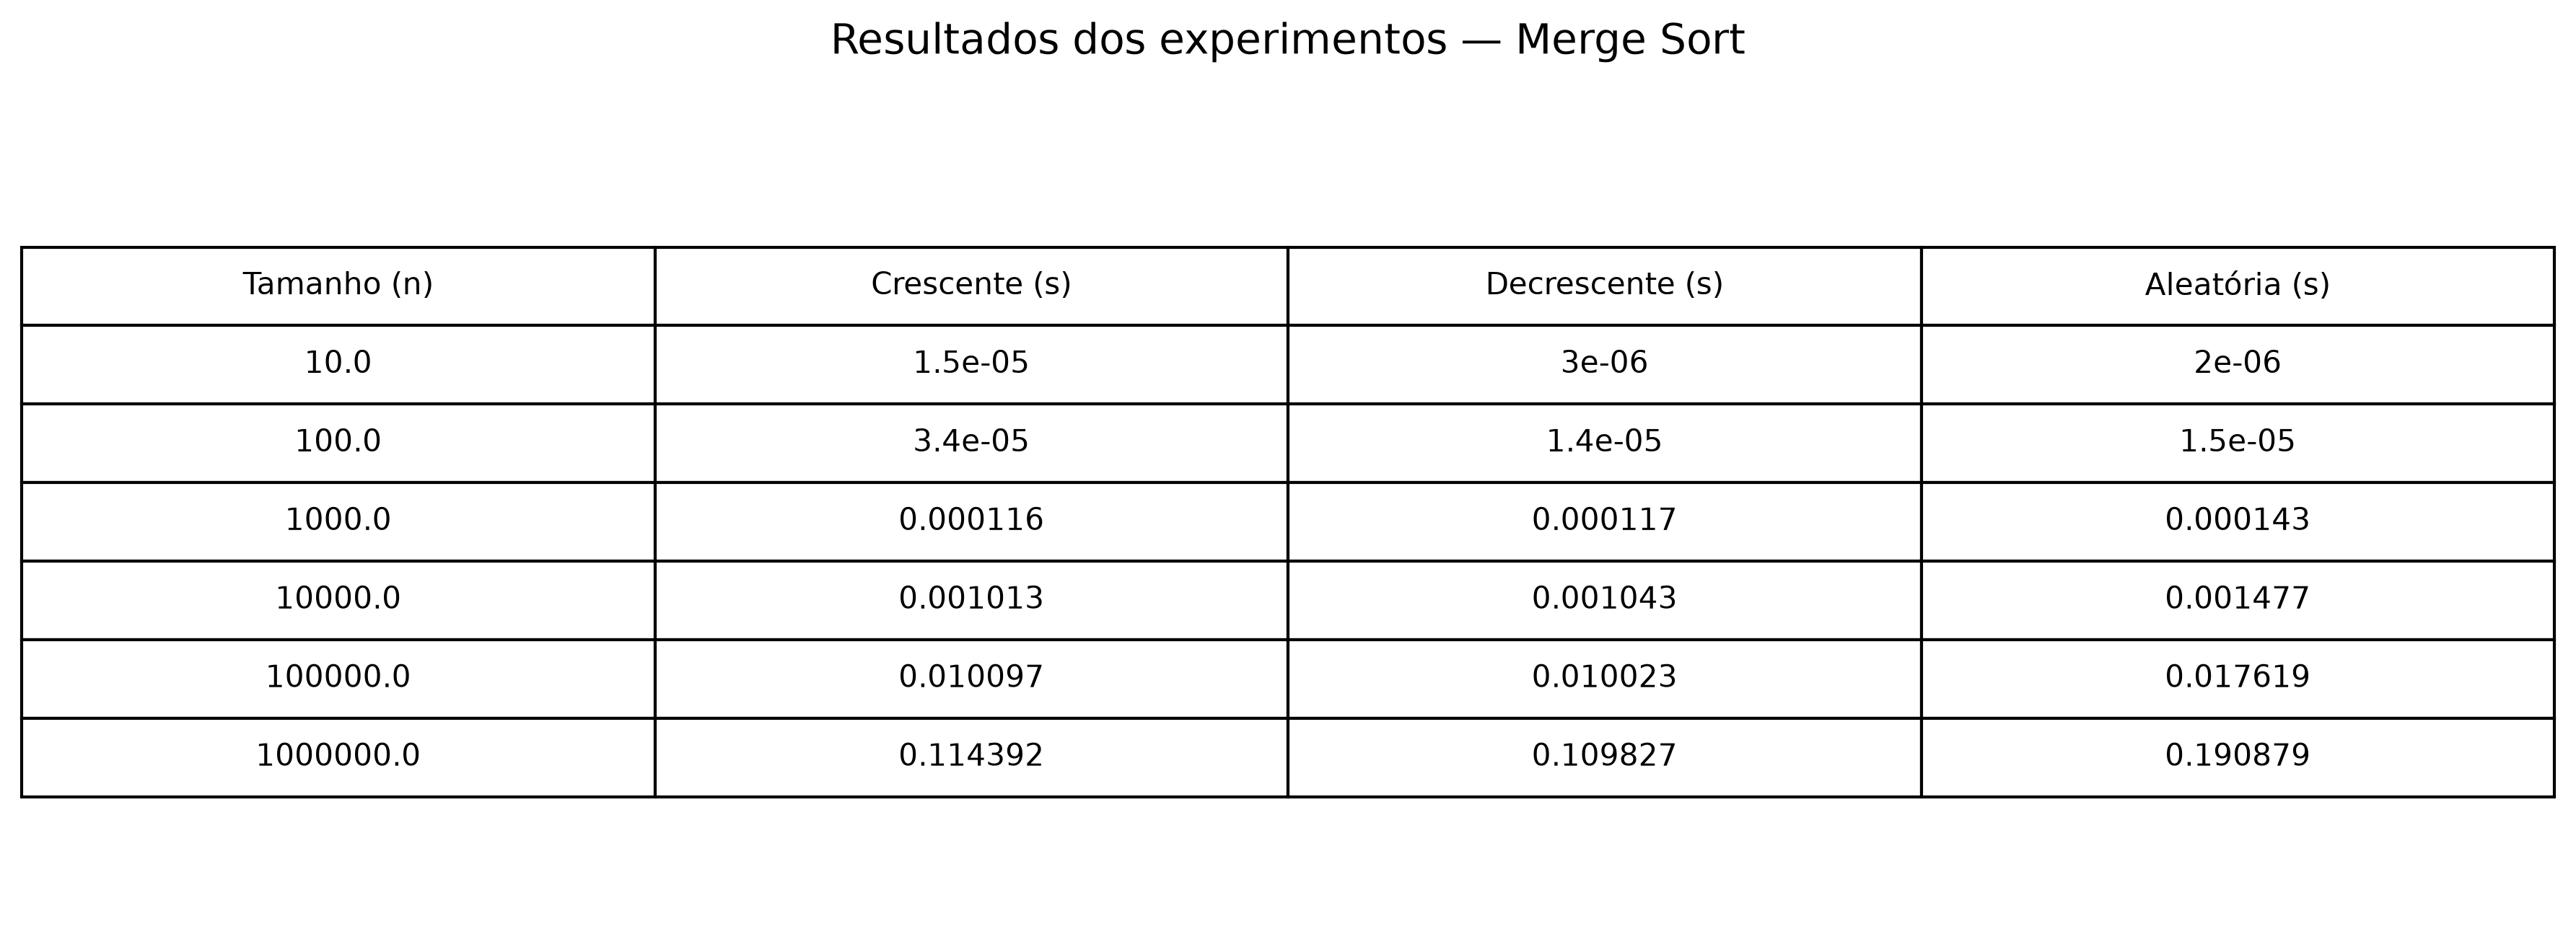
\includegraphics[width=16cm]{Imagens/Merge_Sort/tabela.png}
    \caption{Tabela de tempo de execução do algoritmo Merge Sort}
    \label{fig:tabela-merge}
\end{figure}

\begin{figure}[H]
    \centering
    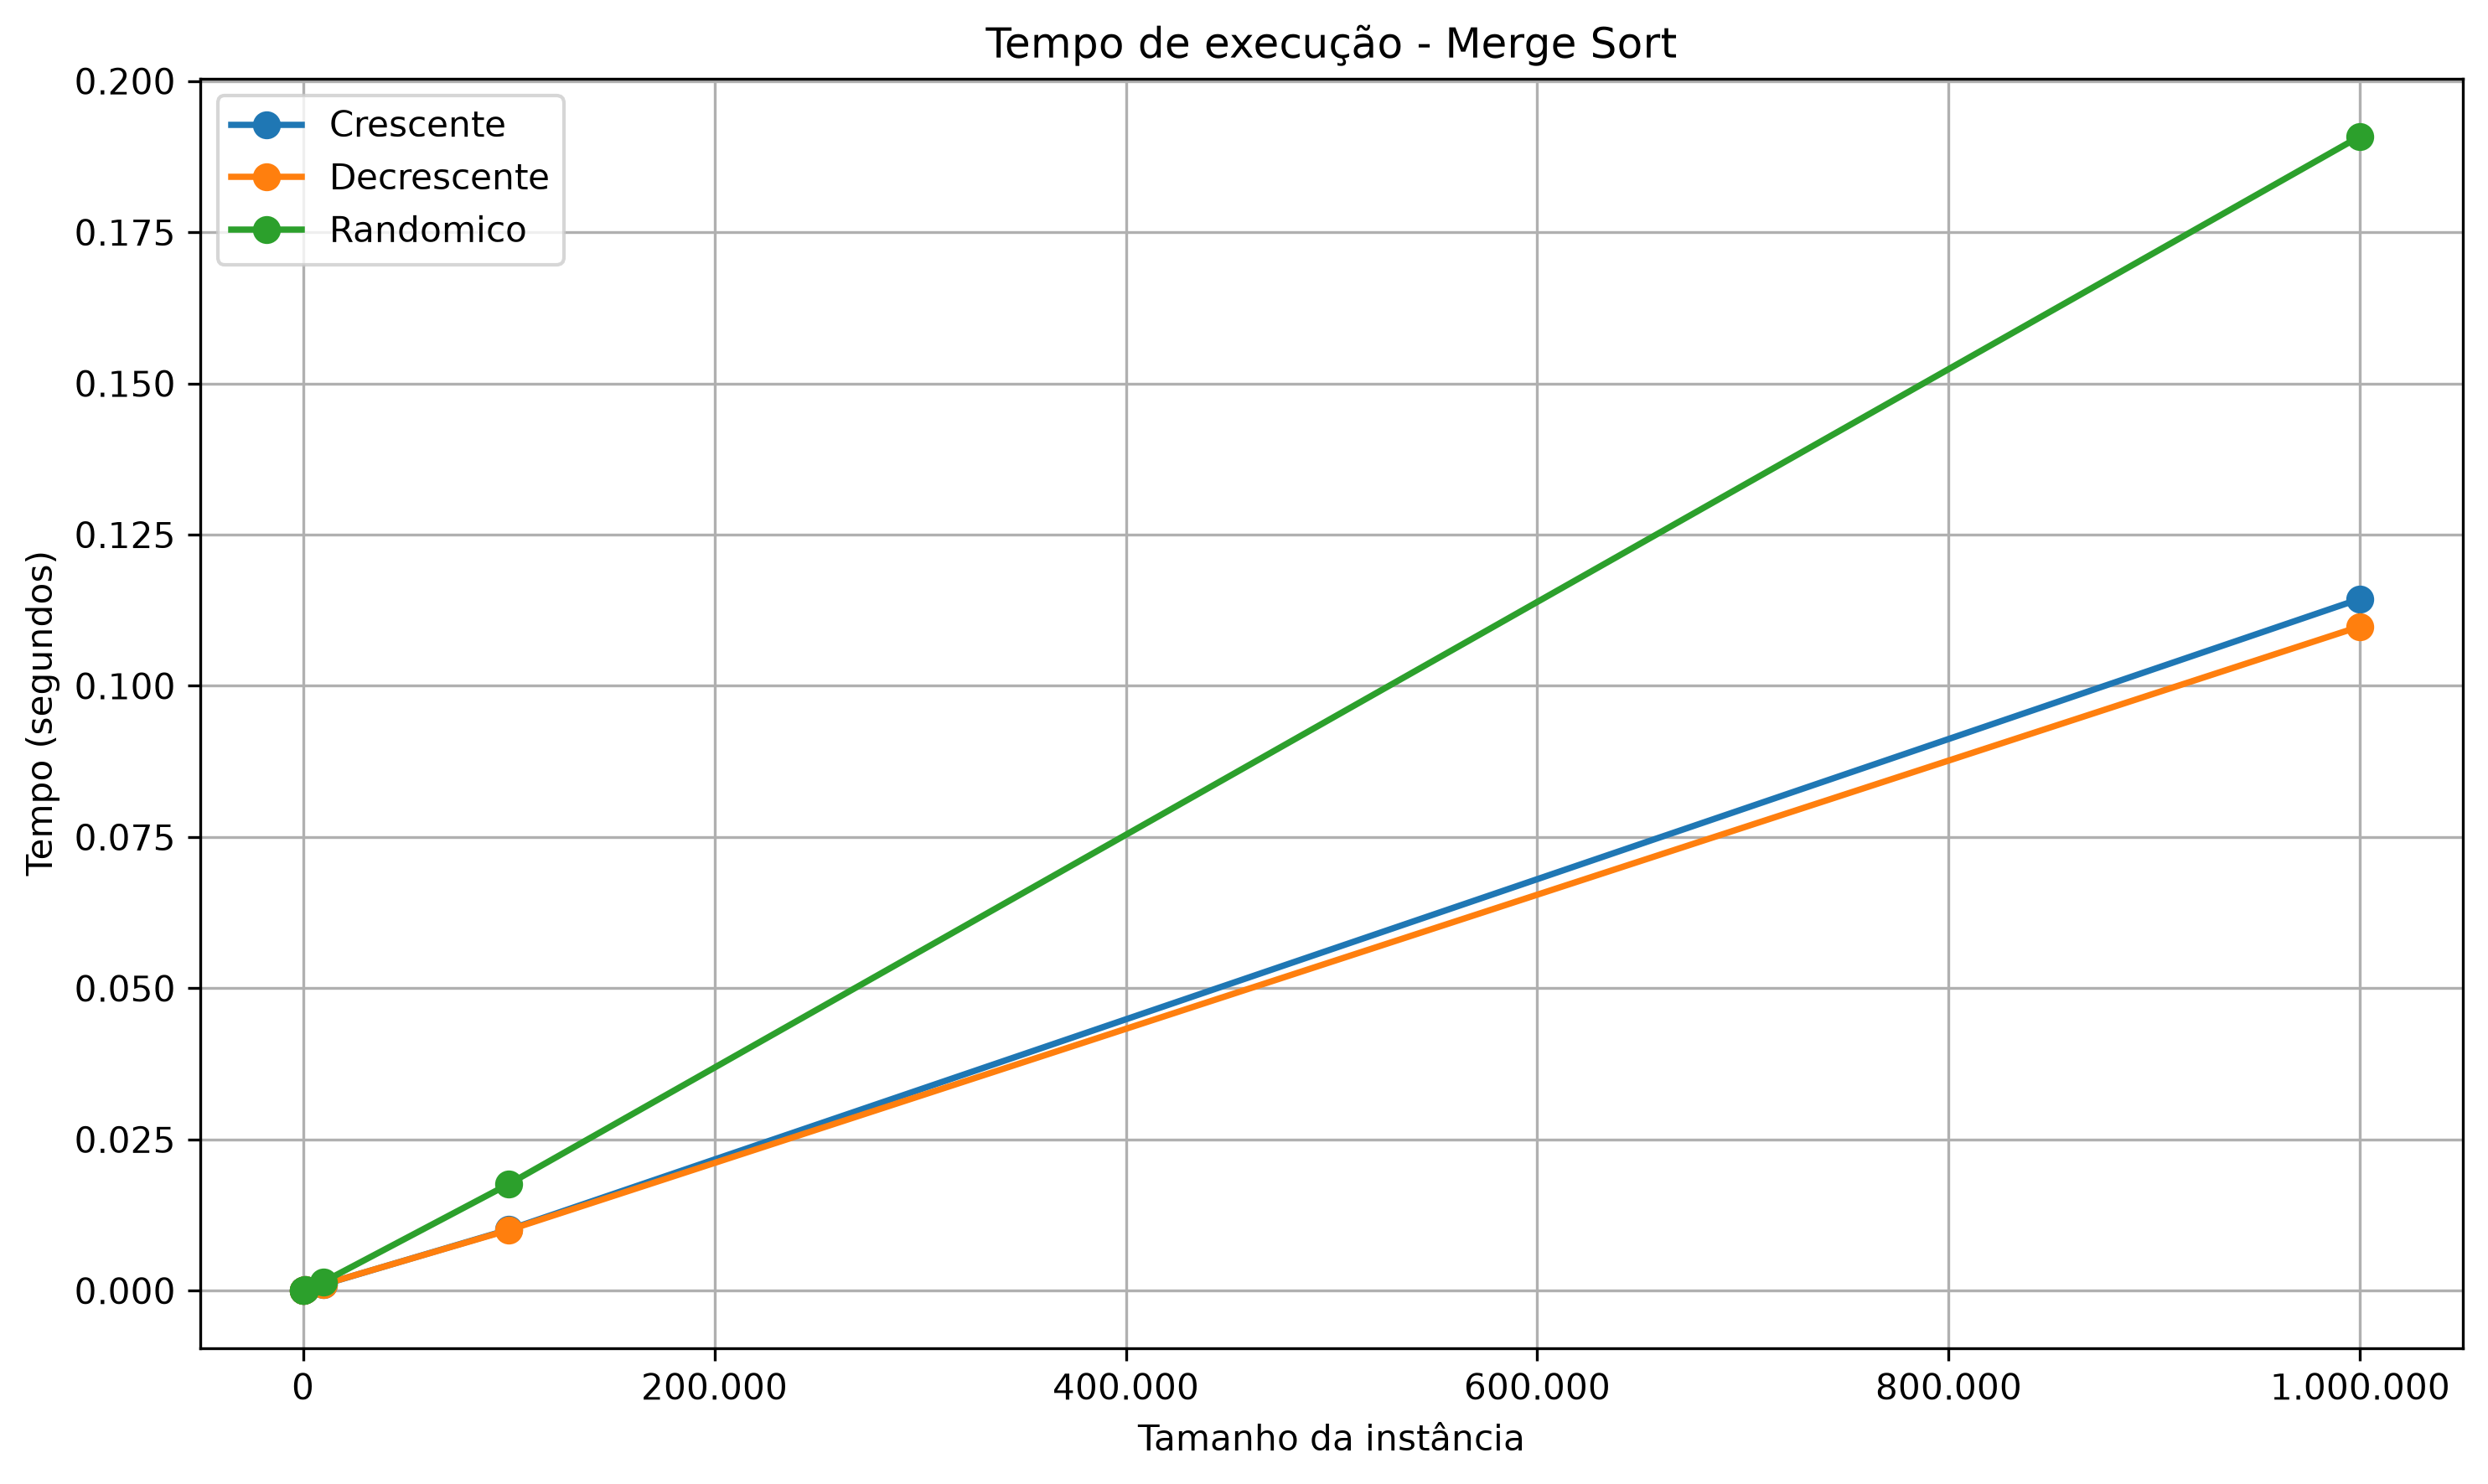
\includegraphics[width=10cm]{Imagens/Merge_Sort/grafico.png}
    \caption{Gráfico de tempo de execução do algoritmo Merge Sort}
    \label{fig:grafico-merge}
\end{figure}

Os resultados obtidos nos experimentos estão apresentados na tabela e no
gráfico. Observa-se que o algoritmo Merge Sort apresenta comportamento
semelhante para as entradas crescentes, decrescentes e aleatórias, pois
sua estratégia de divisão e conquista não depende significativamente
da organização inicial dos elementos.

Durante a execução, o vetor é dividido recursivamente em partes menores
e, posteriormente, essas partes são intercaladas em ordem crescente.
Como todos os elementos precisam ser processados durante as etapas de
intercalação, o algoritmo apresenta complexidade temporal
$\Theta(n\log n)$ nos casos analisados.

Os resultados também permitem observar que o aumento do tamanho da
entrada provoca um crescimento no tempo de execução. Entretanto, esse
crescimento tende a ser menos acentuado do que o observado nos algoritmos
com complexidade quadrática, especialmente para vetores de grandes
dimensões.

Além disso, a implementação utiliza vetores auxiliares durante a
intercalação dos elementos, necessitando de memória adicional
proporcional ao tamanho da entrada. Dessa forma, o Merge Sort apresenta
um bom desempenho para grandes conjuntos de dados, embora utilize mais
memória auxiliar do que algoritmos como o Insertion Sort.


\subsection{Quick Sort}
\begin{figure}[H]
    \centering
    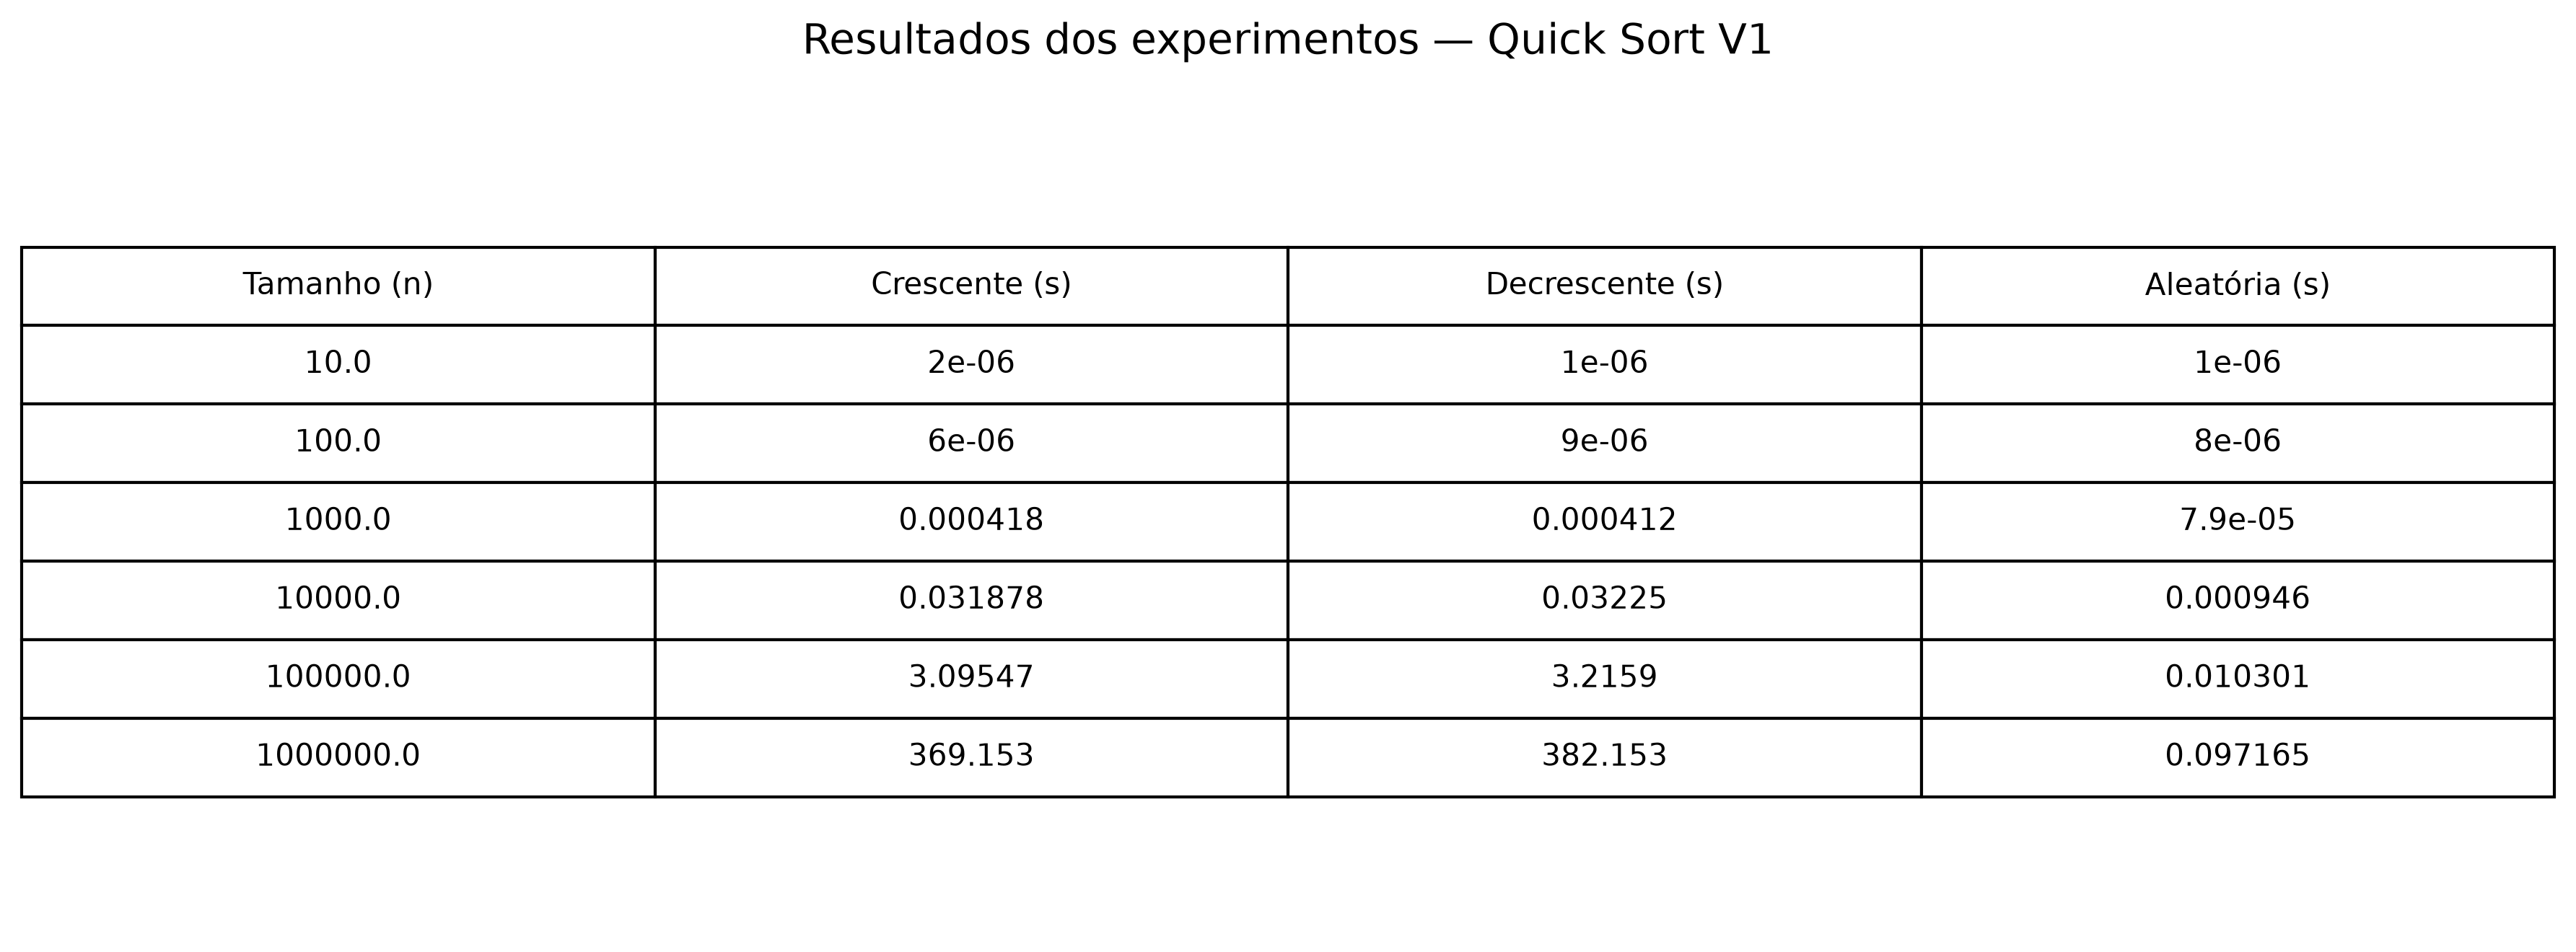
\includegraphics[width=16cm]{Imagens/Quick_Sort/tabela_v1.png}
    \caption{Tabela de tempo de execução do algoritmo Quick Sort (versão 1, pivô no primeiro elemento)}
    \label{fig:tabela-quick-v1}
\end{figure}

\begin{figure}[H]
    \centering
    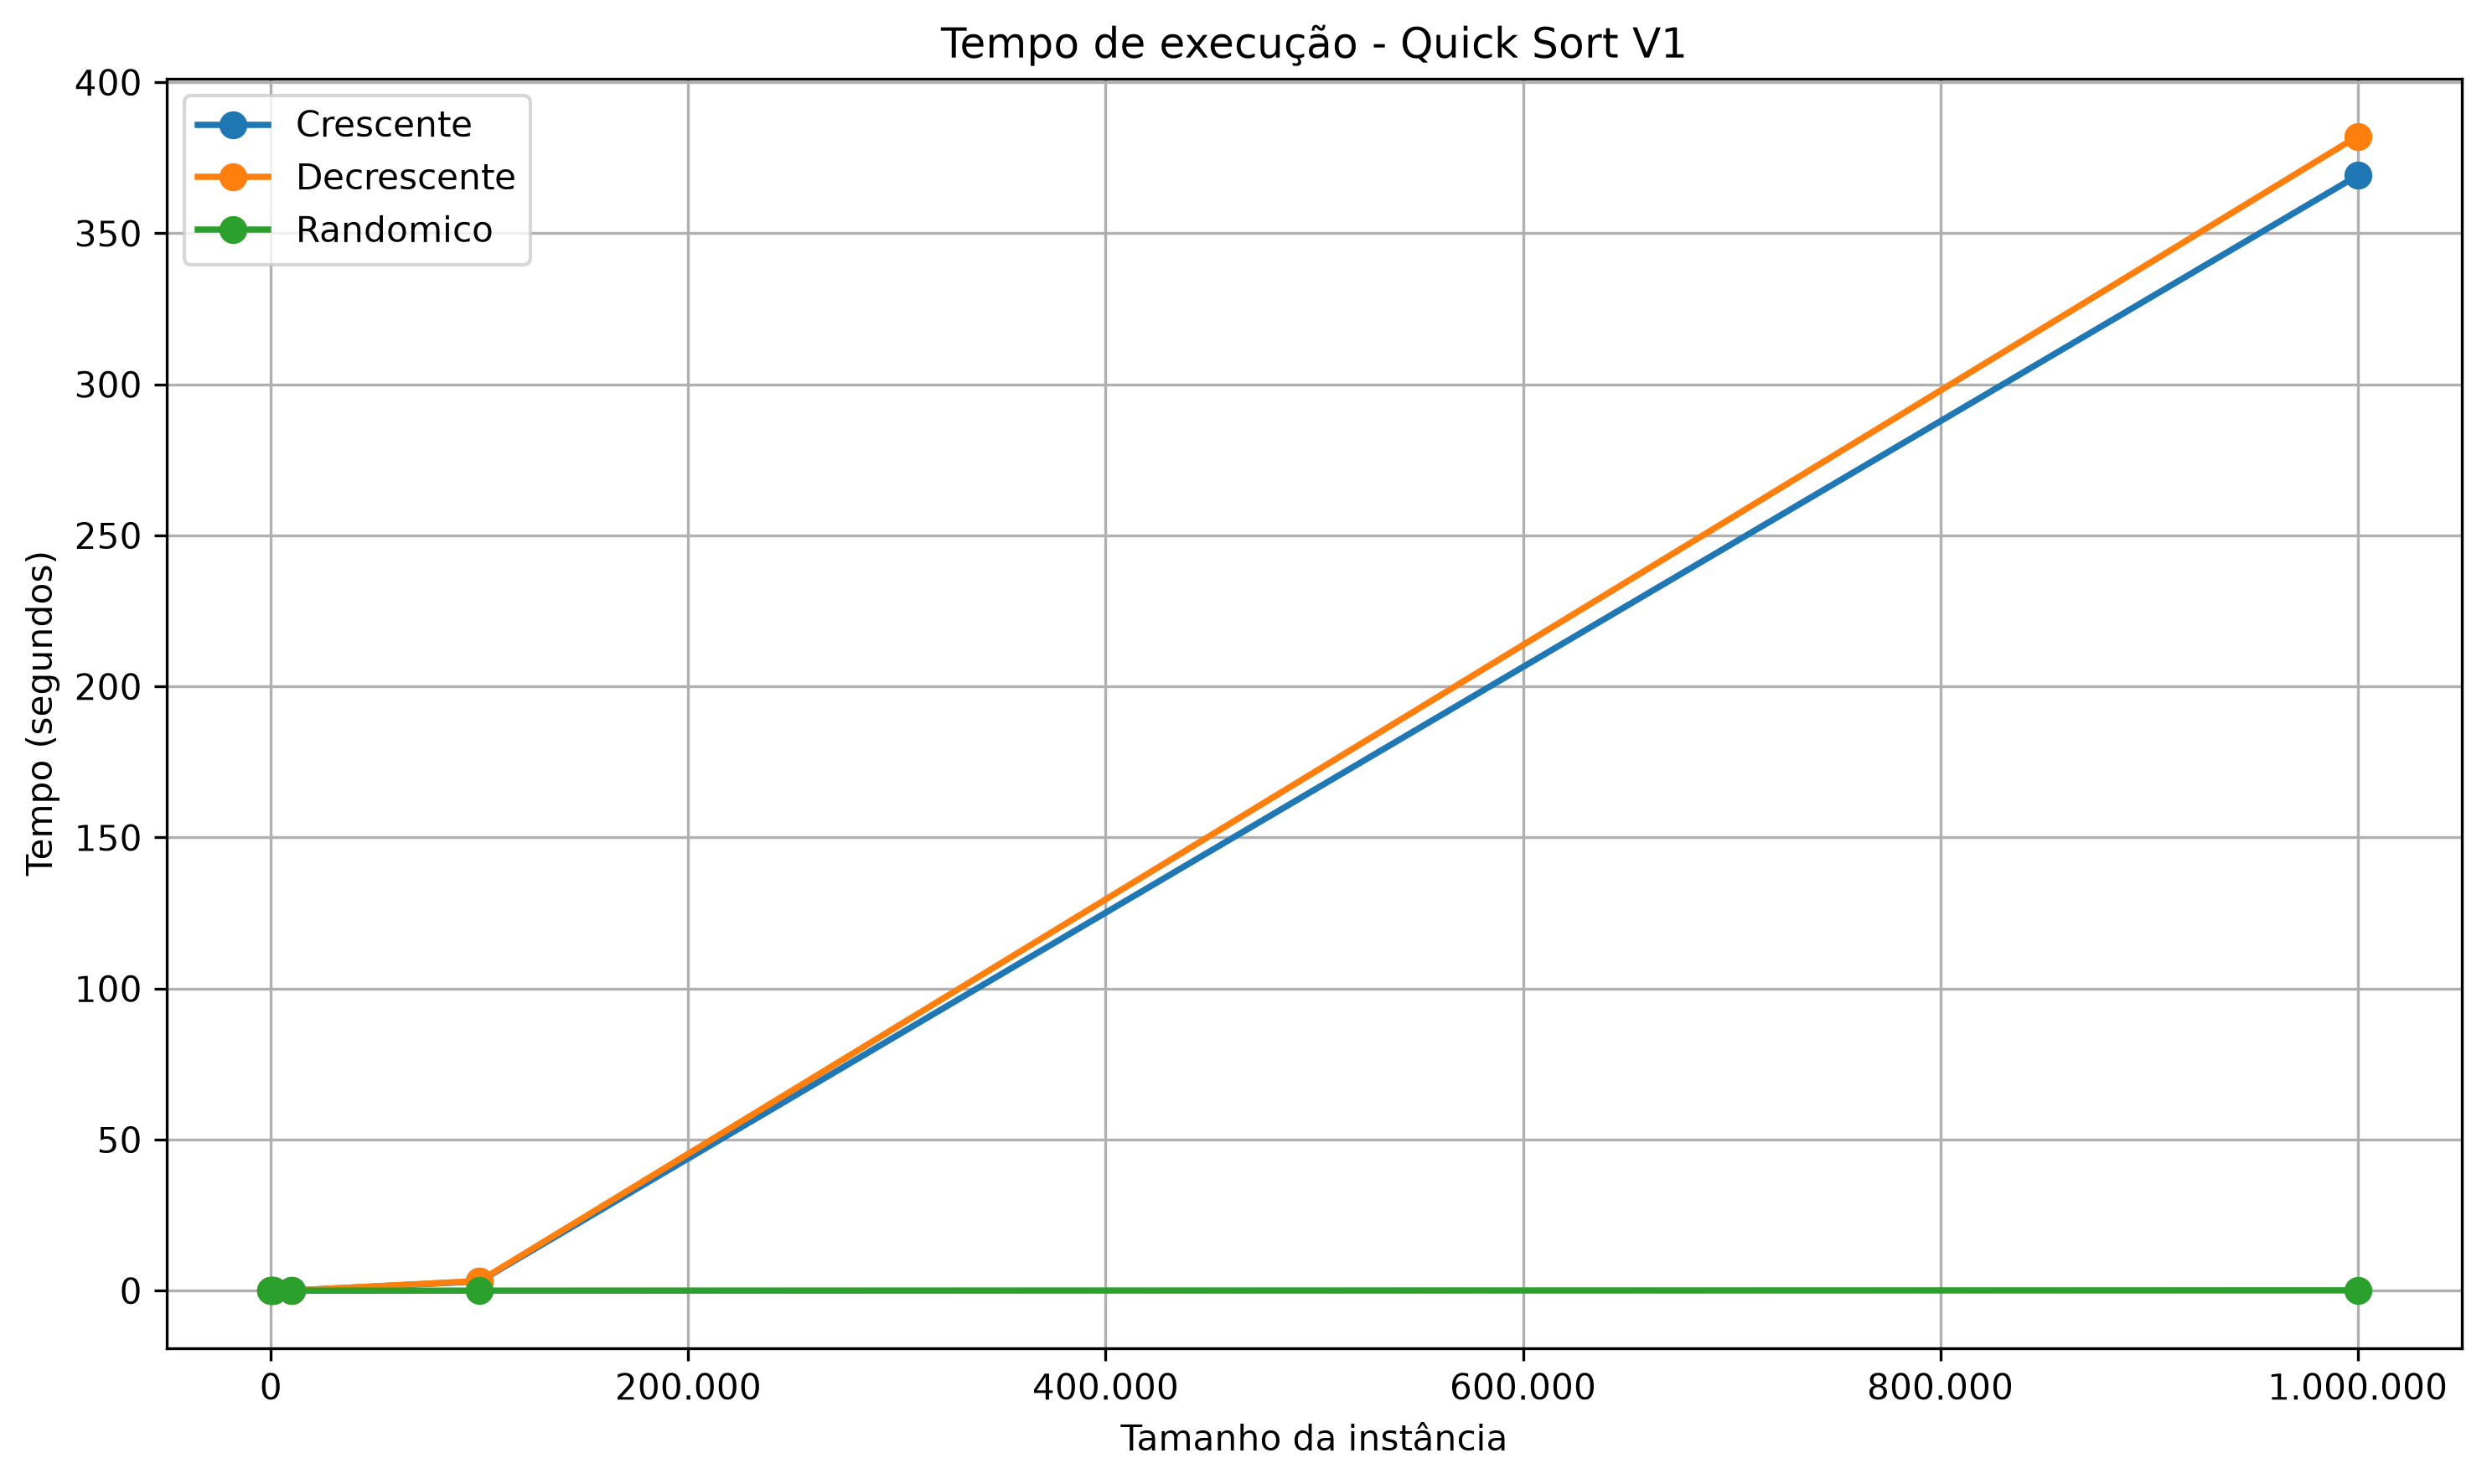
\includegraphics[width=10cm]{Imagens/Quick_Sort/grafico_v1.png}
    \caption{Gráfico de tempo de execução do algoritmo Quick Sort (versão 1, pivô no primeiro elemento)}
    \label{fig:grafico-quick-v1}
\end{figure}

\begin{figure}[H]
    \centering
    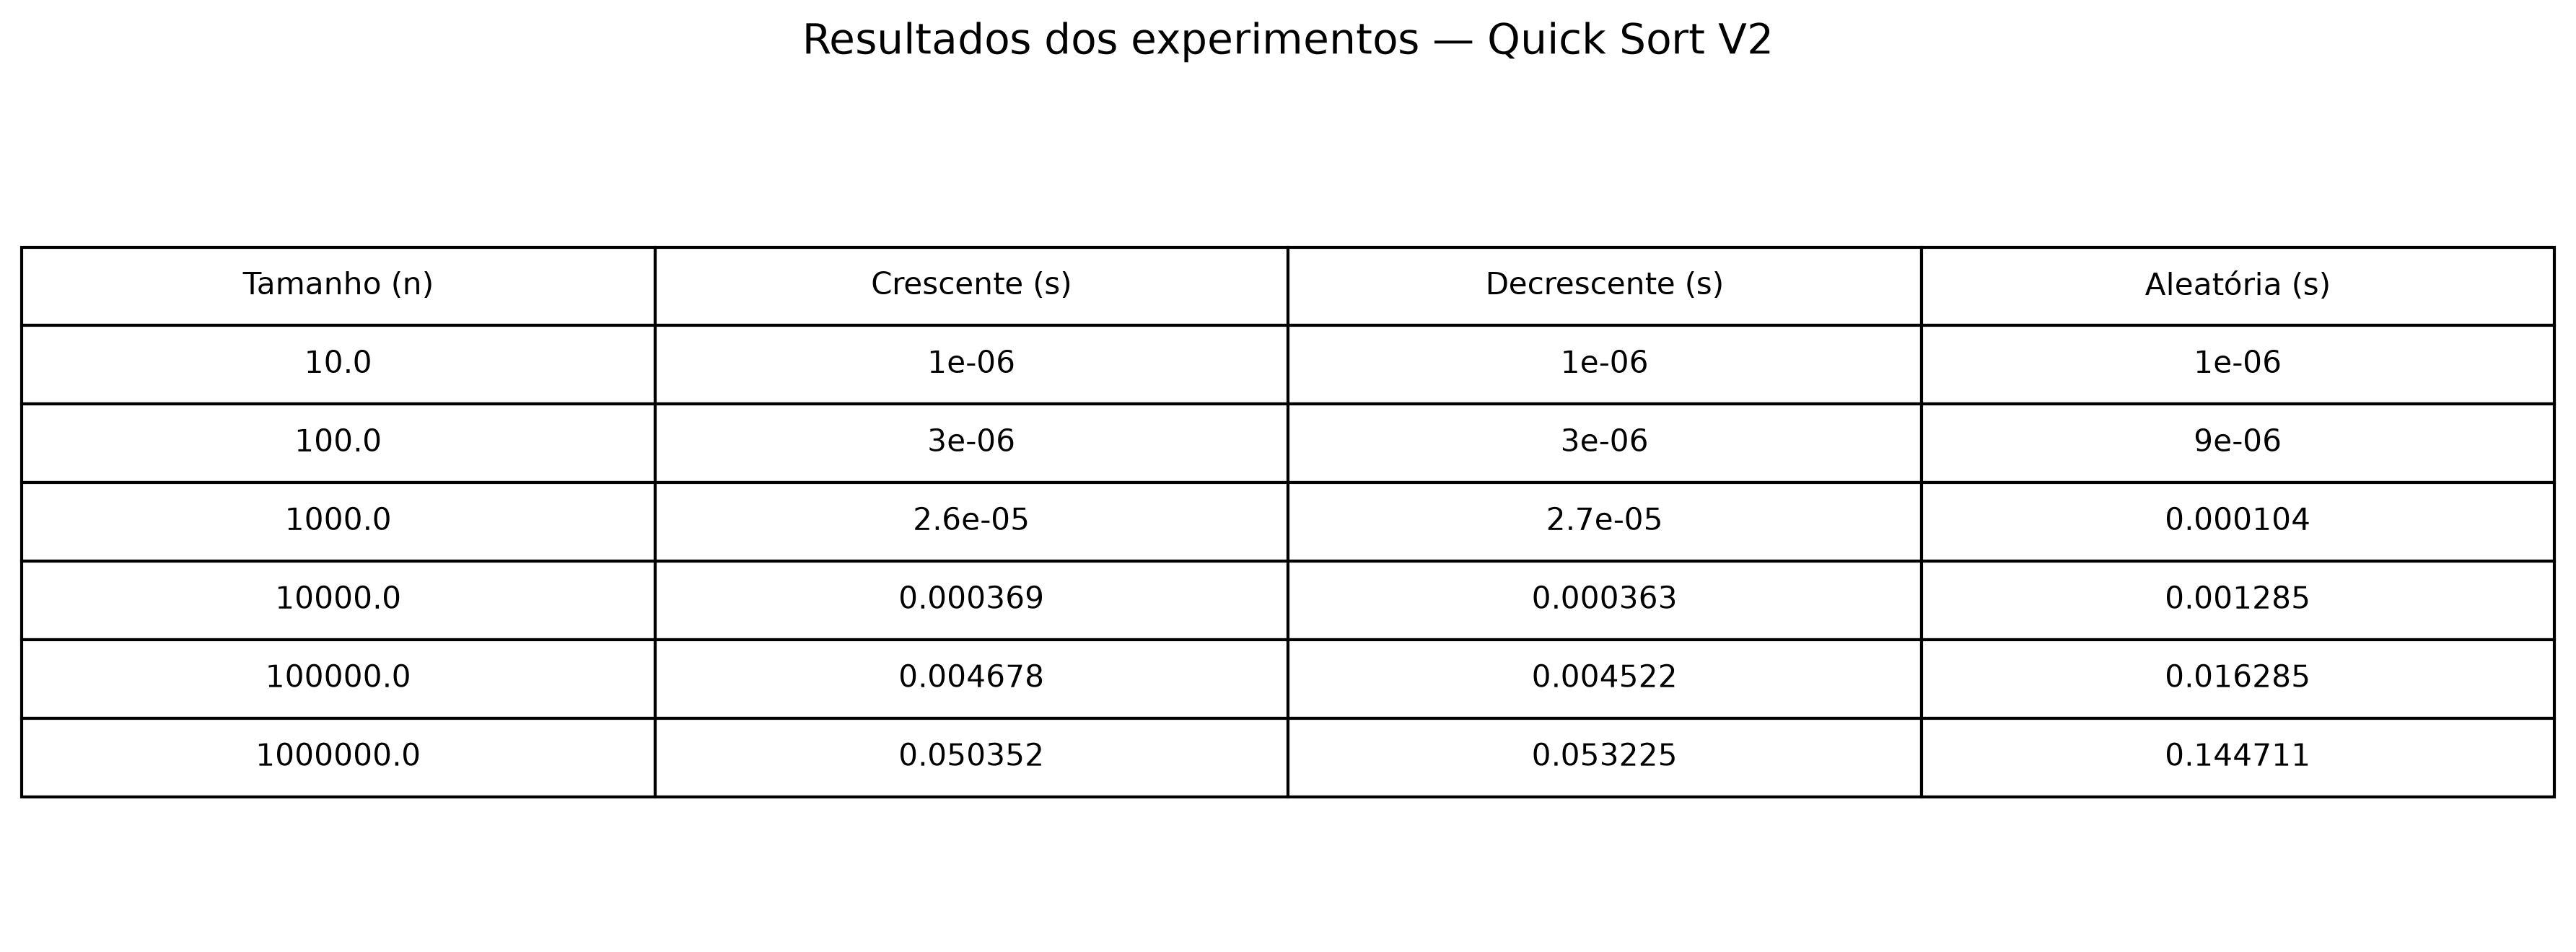
\includegraphics[width=16cm]{Imagens/Quick_Sort/tabela_v2.png}
    \caption{Tabela de tempo de execução do algoritmo Quick Sort (versão 2, pivô pela média aritmética)}
    \label{fig:tabela-quick-v2}
\end{figure}

\begin{figure}[H]
    \centering
    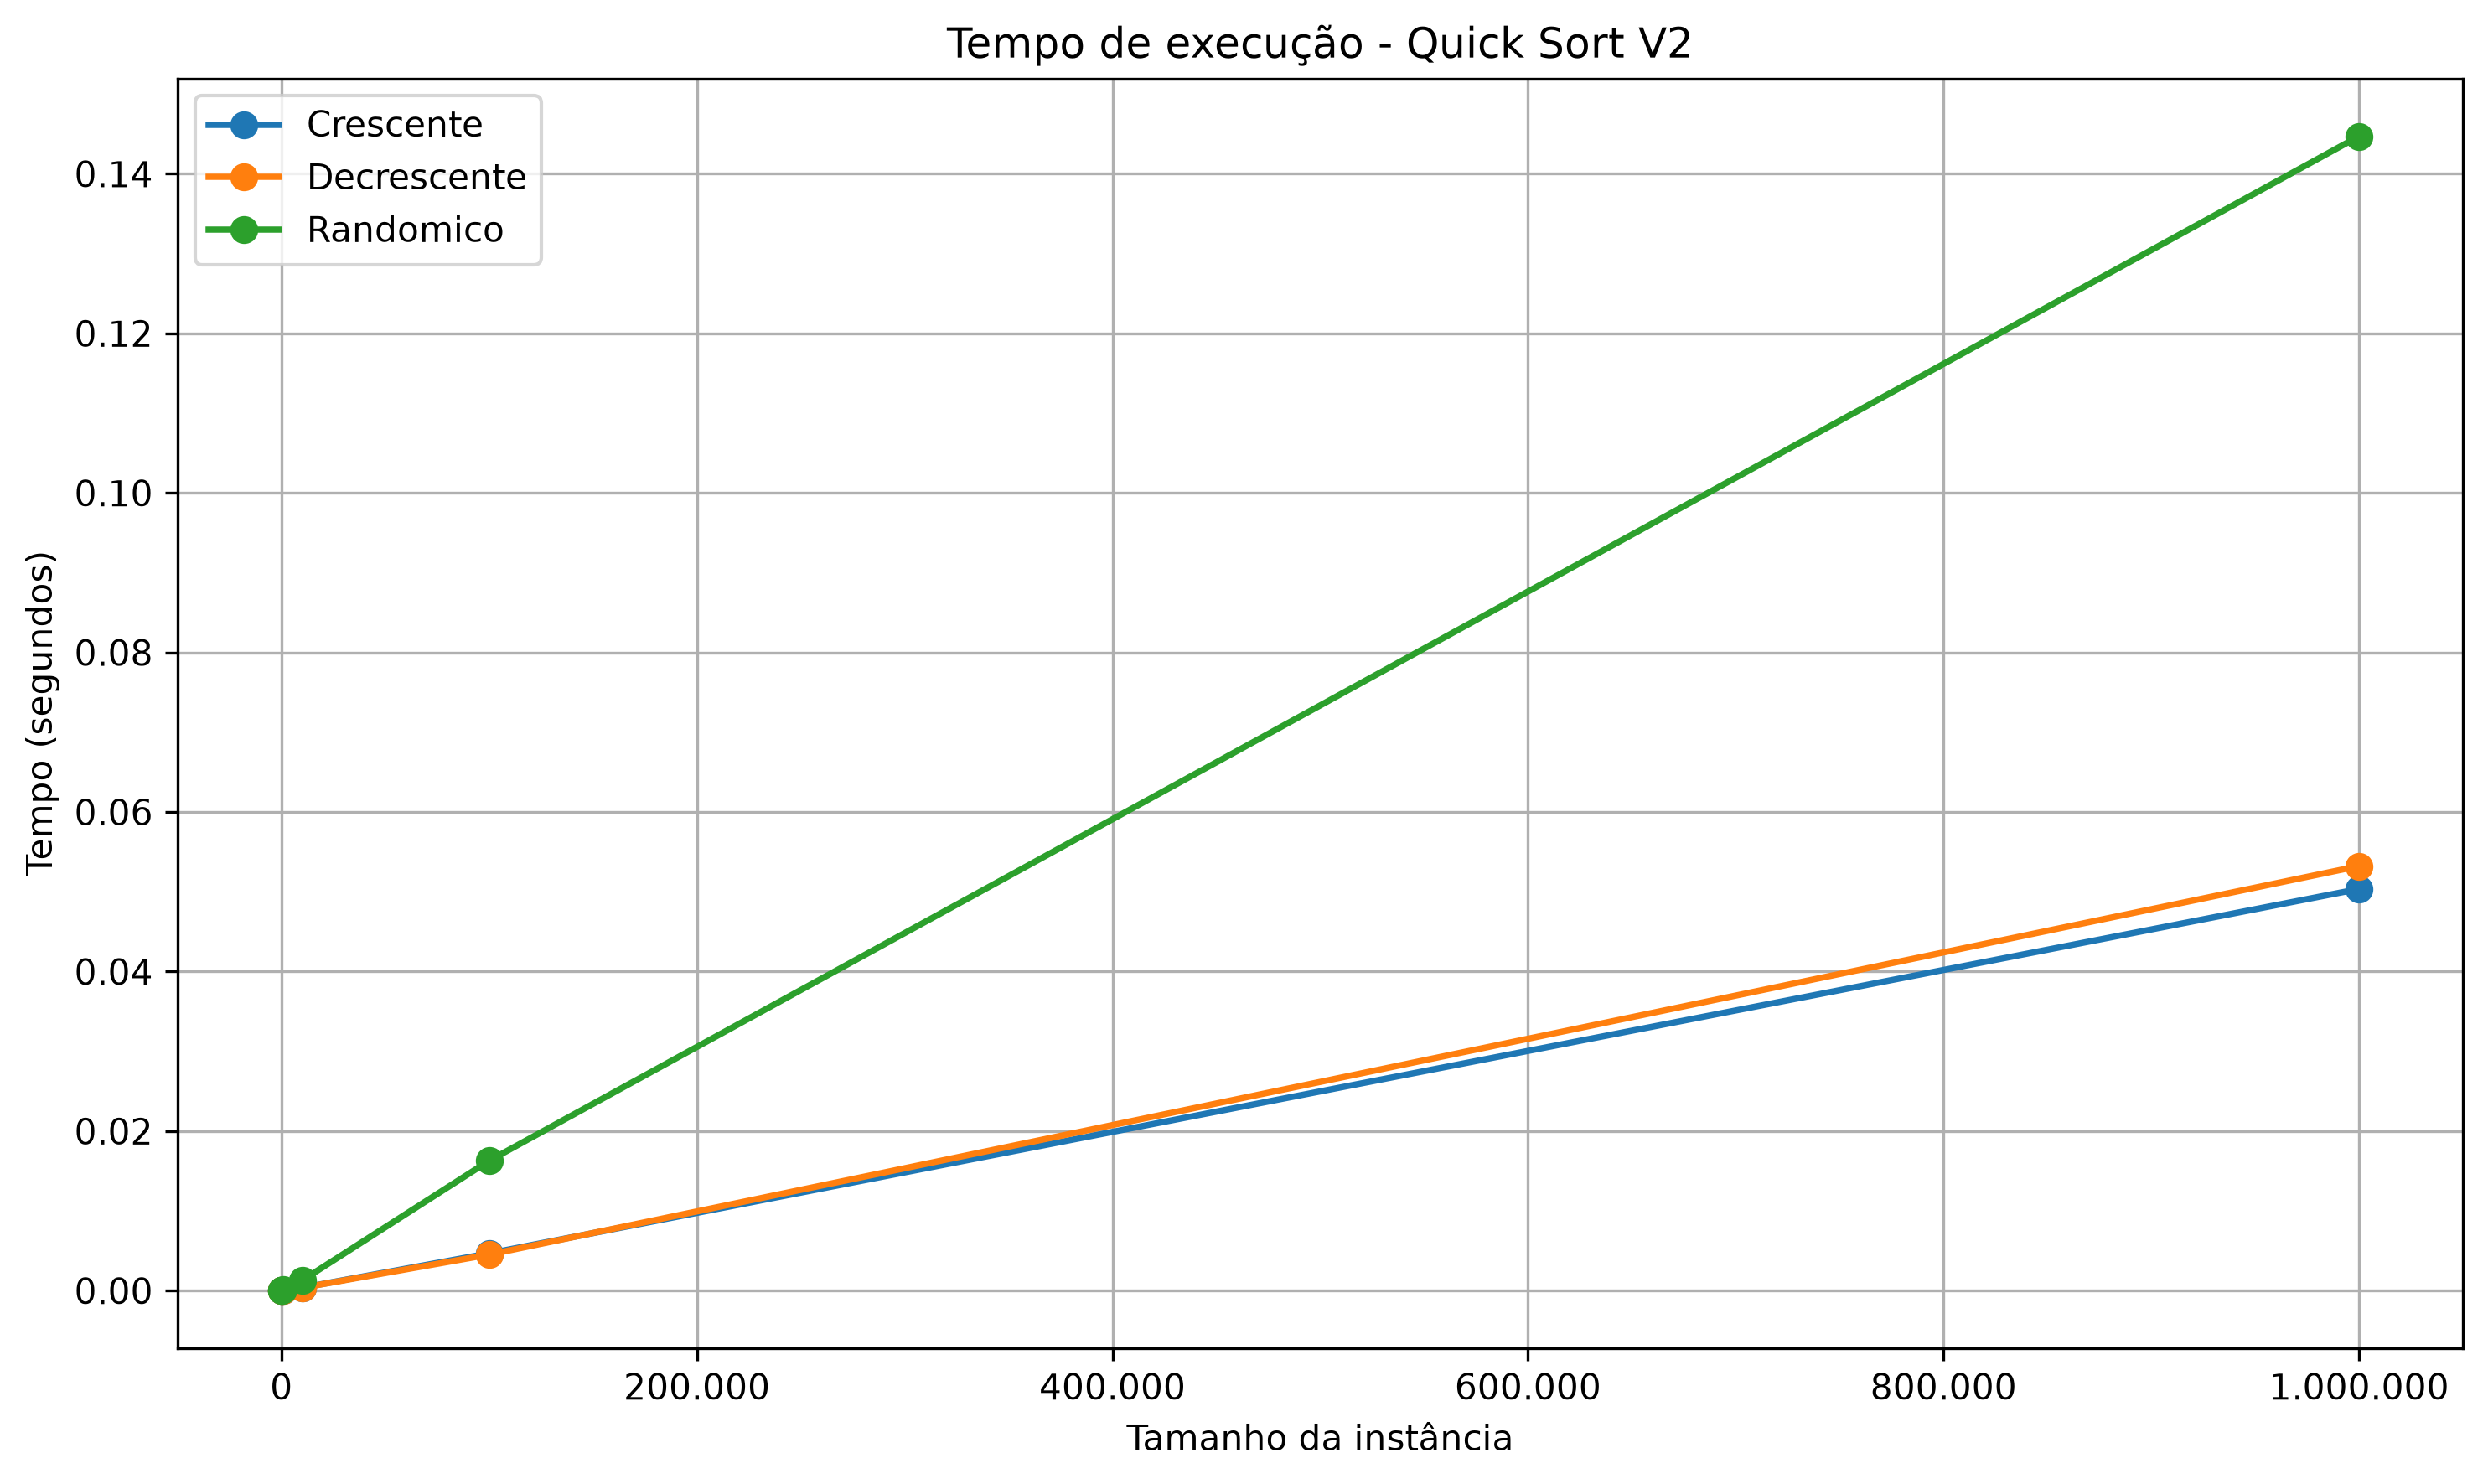
\includegraphics[width=10cm]{Imagens/Quick_Sort/grafico_v2.png}
    \caption{Gráfico de tempo de execução do algoritmo Quick Sort (versão 2, pivô pela média aritmética)}
    \label{fig:grafico-quick-v2}
\end{figure}

Os resultados obtidos nos experimentos estão apresentados nas tabelas e
nos gráficos de cada versão. Diferentemente do Merge Sort, o desempenho
do Quick Sort depende da organização inicial dos elementos, pois ela
influencia a escolha do pivô e, consequentemente, o balanceamento das
partições geradas a cada particionamento.

Na versão 1, o pivô é sempre o primeiro elemento da partição. Para
entradas aleatórias, é esperado que as partições fiquem razoavelmente
equilibradas, resultando em um comportamento próximo de
$\Theta(n\log n)$. Já para entradas crescentes e decrescentes, o pivô
tende a ser o menor ou o maior elemento da partição, gerando partições
muito desiguais e aproximando o algoritmo do pior caso, com complexidade
$\Theta(n^2)$. Esse efeito pode ser observado na
Figura~\ref{fig:grafico-quick-v1}, em que o tempo de execução dessas
entradas cresce de forma mais acentuada com o aumento do tamanho do
vetor.

Na versão 2, o pivô é a média aritmética dos elementos da partição. Como
a média tende a ficar próxima do centro dos valores quando eles estão
distribuídos de forma uniforme, as entradas crescentes e decrescentes
deixam de gerar partições tão desbalanceadas, e o tempo de execução
dessas entradas se aproxima do observado para entradas aleatórias, como
mostra a Figura~\ref{fig:grafico-quick-v2}. Em contrapartida, o cálculo
da média exige percorrer toda a partição a cada chamada, o que acrescenta
um custo linear adicional ao particionamento.

Comparando as duas versões, observa-se que a versão 2 reduz a
sensibilidade do algoritmo à ordem inicial do vetor, enquanto a versão 1
é mais simples e não possui custo adicional para a escolha do pivô, mas
é mais prejudicada por entradas já ordenadas. Para entradas aleatórias,
as duas versões apresentam comportamento semelhante, com a versão 2
ligeiramente mais custosa devido ao cálculo da média.

Além disso, o algoritmo realiza a ordenação no próprio vetor, sem
necessidade de vetores auxiliares. A implementação realiza a chamada
recursiva apenas sobre a menor partição, o que limita a profundidade da
pilha de recursão a, no máximo, proporcional a $\log_2 n$. Dessa forma,
o Quick Sort utiliza menos memória auxiliar do que o Merge Sort, embora
possa apresentar desempenho inferior em seu pior caso.

\newpage

% --------------------------------------------------
% COMPARAÇÃO ENTRE OS ALGORITMOS
% --------------------------------------------------

\section{COMPARAÇÃO ENTRE OS ALGORITMOS}

Além da análise individual de cada algoritmo, foram realizados
experimentos comparativos entre o Insertion Sort, Bubble Sort,
Selection Sort, Shell Sort, Merge Sort e Quick Sort (em 2 versões diferentes)
considerando os três tipos de entrada utilizados nos experimentos: 
crescente, decrescente e aleatória.

\subsection{Entrada crescente}
A Figura~\ref{fig:comparacao_crescente} apresenta a comparação entre
os sete algoritmos para entradas inicialmente ordenadas de forma
crescente.

\begin{figure}[H]
    \centering
    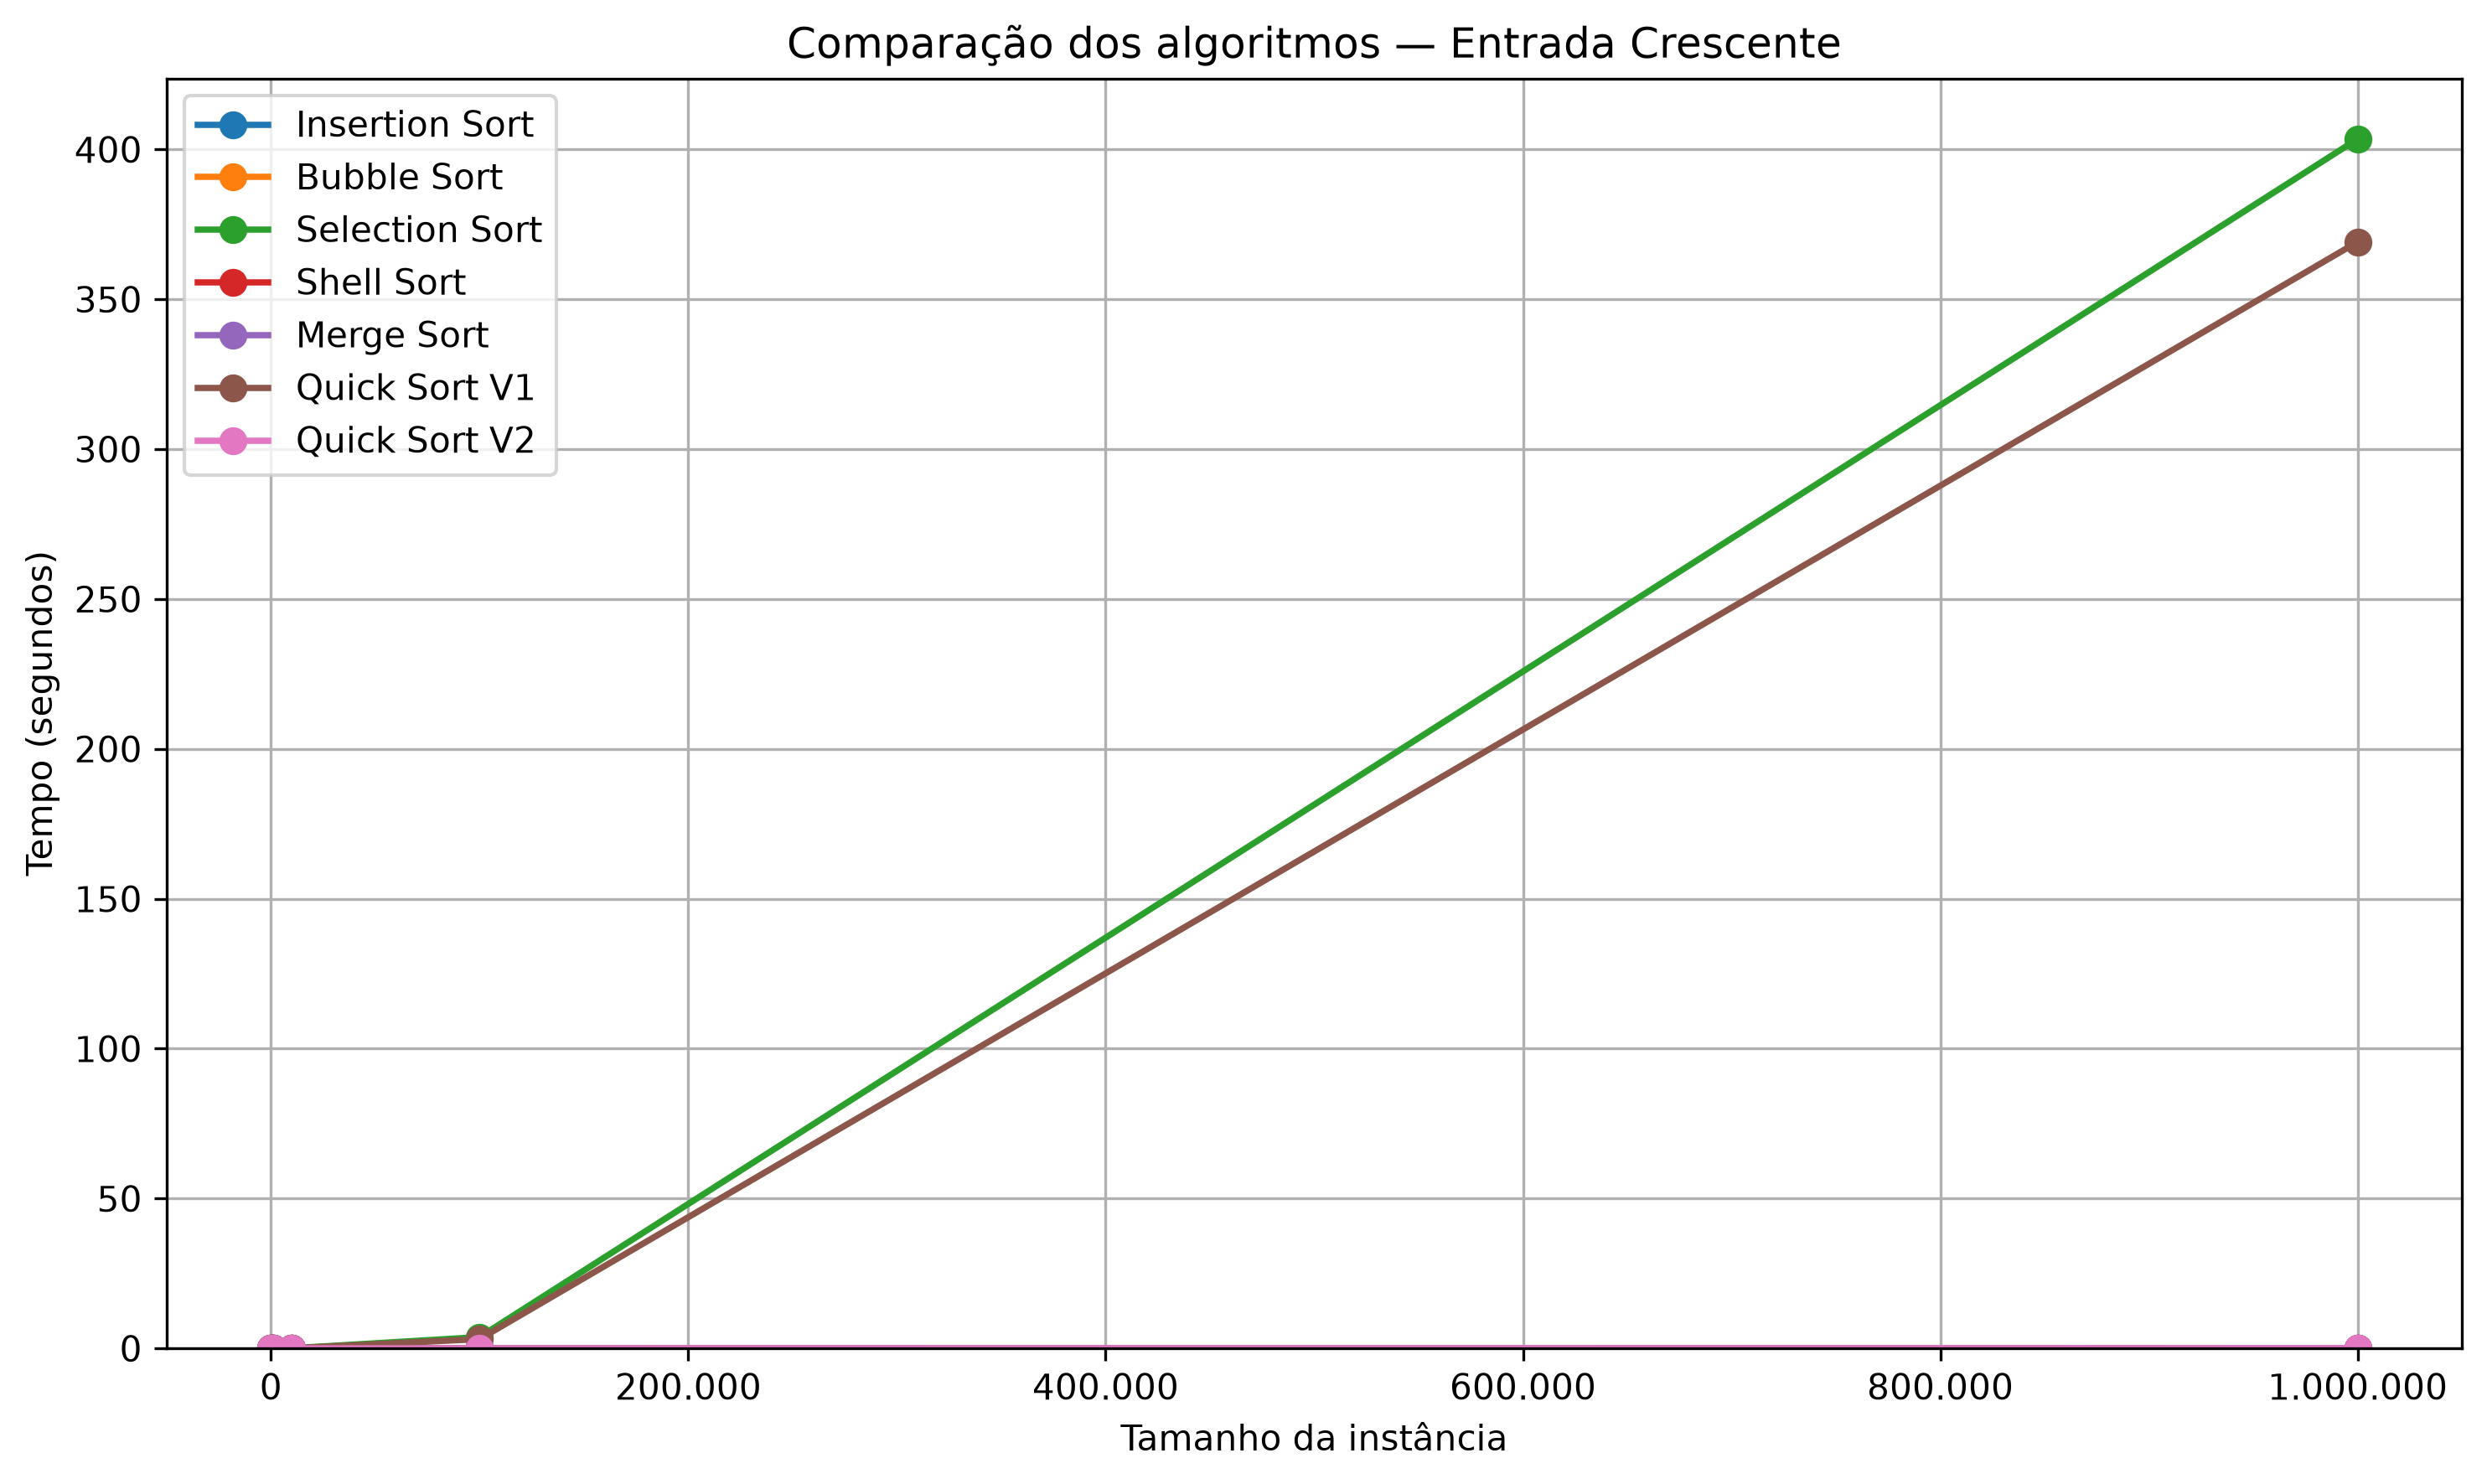
\includegraphics[width=\textwidth,keepaspectratio]{Imagens/Comparacoes/comparacao_crescente.png}
    \caption{Comparação dos algoritmos para entrada crescente.}
    \label{fig:comparacao_crescente}
\end{figure}

Nesse tipo de entrada, apenas dois algoritmos apresentaram tempos
elevados: o \textit{Selection Sort}, com cerca de 400 segundos para
1.000.000 de elementos, e o \textit{Quick Sort} versão 1, com cerca de
370 segundos. O \textit{Selection Sort} mantém uma quantidade quadrática
de comparações mesmo com o vetor já ordenado, pois sempre percorre a
parte não ordenada para localizar o menor elemento. Já o \textit{Quick
Sort} versão 1 utiliza o primeiro elemento como pivô, que em um vetor
crescente é sempre o menor valor da partição. Dessa forma, cada
particionamento separa apenas um elemento, e o algoritmo se comporta de
acordo com o pior caso, $\Theta(n^2)$.

O \textit{Insertion Sort} e o \textit{Bubble Sort} apresentaram tempos
praticamente nulos na escala do gráfico, pois, em vetores já ordenados,
o primeiro não precisa deslocar elementos e o segundo é interrompido
antecipadamente quando não ocorrem trocas, ambos com custo linear. O
\textit{Shell Sort} e o \textit{Merge Sort} também apresentaram tempos
muito baixos, compatíveis com a complexidade próxima de $\Theta(n\log n)$.

A versão 2 do \textit{Quick Sort} não sofreu a degradação observada na
versão 1. Como a média aritmética de valores distribuídos
uniformemente fica próxima do centro da partição, as partições
permaneceram equilibradas mesmo com o vetor ordenado, e o tempo de
execução foi comparável ao do \textit{Merge Sort}. Esse resultado mostra
que a escolha do pivô é decisiva para o desempenho do algoritmo.


\subsection{Entrada decrescente}
A Figura~\ref{fig:comparacao_decrescente} apresenta a comparação entre
os sete algoritmos para entradas inicialmente organizadas em ordem
decrescente.

\begin{figure}[H]
    \centering
    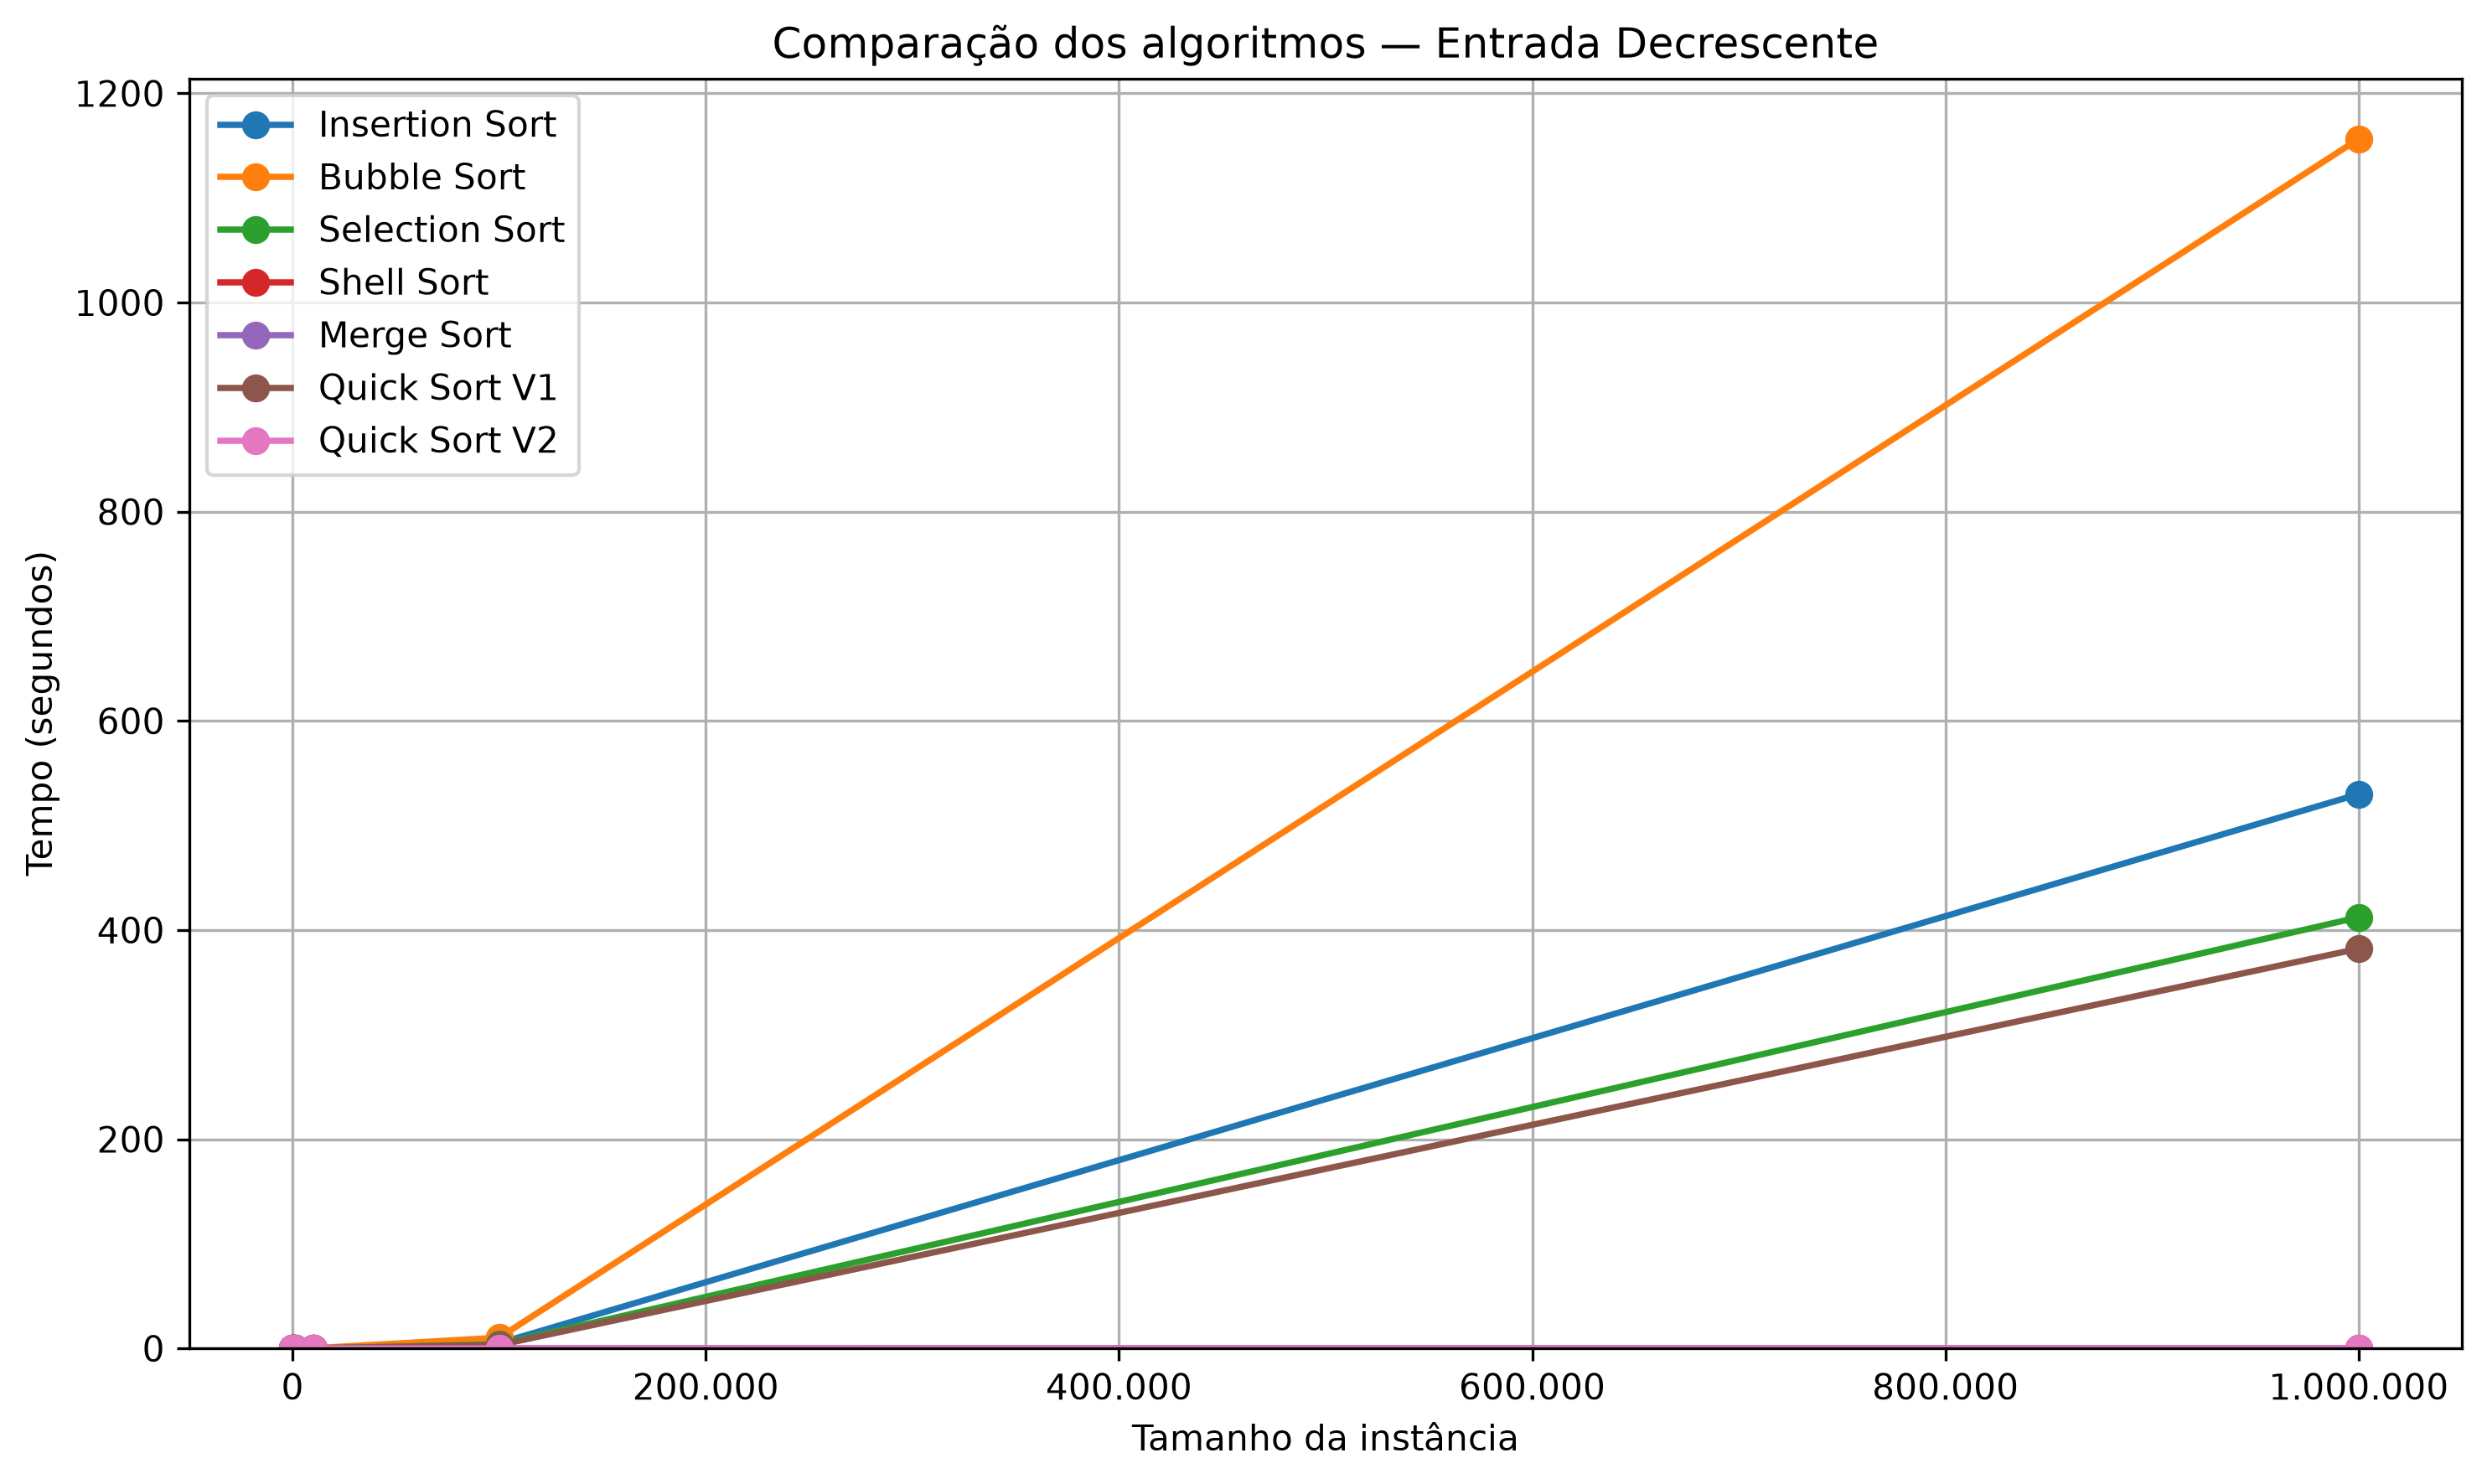
\includegraphics[width=\textwidth,keepaspectratio]{Imagens/Comparacoes/comparacao_decrescente.png}
    \caption{Comparação dos algoritmos para entrada decrescente.}
    \label{fig:comparacao_decrescente}
\end{figure}

Nesse caso, quatro algoritmos apresentaram tempos elevados para
1.000.000 de elementos. O \textit{Bubble Sort} foi o mais lento, com
cerca de 1150 segundos, devido à grande quantidade de comparações e
trocas necessárias para inverter completamente o vetor. Em seguida
aparece o \textit{Insertion Sort}, com cerca de 530 segundos, pois cada
novo elemento precisa ser deslocado até o início da parte já ordenada.
Esse valor é aproximadamente o dobro do observado em entradas
aleatórias, o que é coerente com o fato de o número de deslocamentos
no pior caso ser cerca de duas vezes o do caso médio.

O \textit{Selection Sort}, com cerca de 410 segundos, apresentou tempo
muito próximo ao observado nas entradas crescente e aleatória, pois o
número de comparações realizadas não depende da organização inicial do
vetor. O \textit{Quick Sort} versão 1 apresentou cerca de 380 segundos:
em um vetor decrescente, o primeiro elemento é o maior valor da
partição, e o particionamento separa apenas um elemento por vez, o que
leva o algoritmo ao pior caso quadrático.

O \textit{Shell Sort}, o \textit{Merge Sort} e o \textit{Quick Sort}
versão 2 apresentaram tempos muito baixos, praticamente indistinguíveis
do eixo horizontal na escala do gráfico. No caso do \textit{Merge Sort},
isso ocorre porque as etapas de divisão e intercalação são as mesmas
independentemente da disposição inicial dos elementos. Na versão 2 do
\textit{Quick Sort}, a média aritmética manteve as partições
equilibradas, evitando o pior caso observado na versão 1.

\subsection{Entrada aleatória}
A Figura~\ref{fig:comparacao_aleatoria} apresenta a comparação entre
os sete algoritmos implementados (os seis algoritmos estudados, sendo o
\textit{Quick Sort} em suas duas versões) para entradas geradas
aleatoriamente.

\begin{figure}[H]
    \centering
    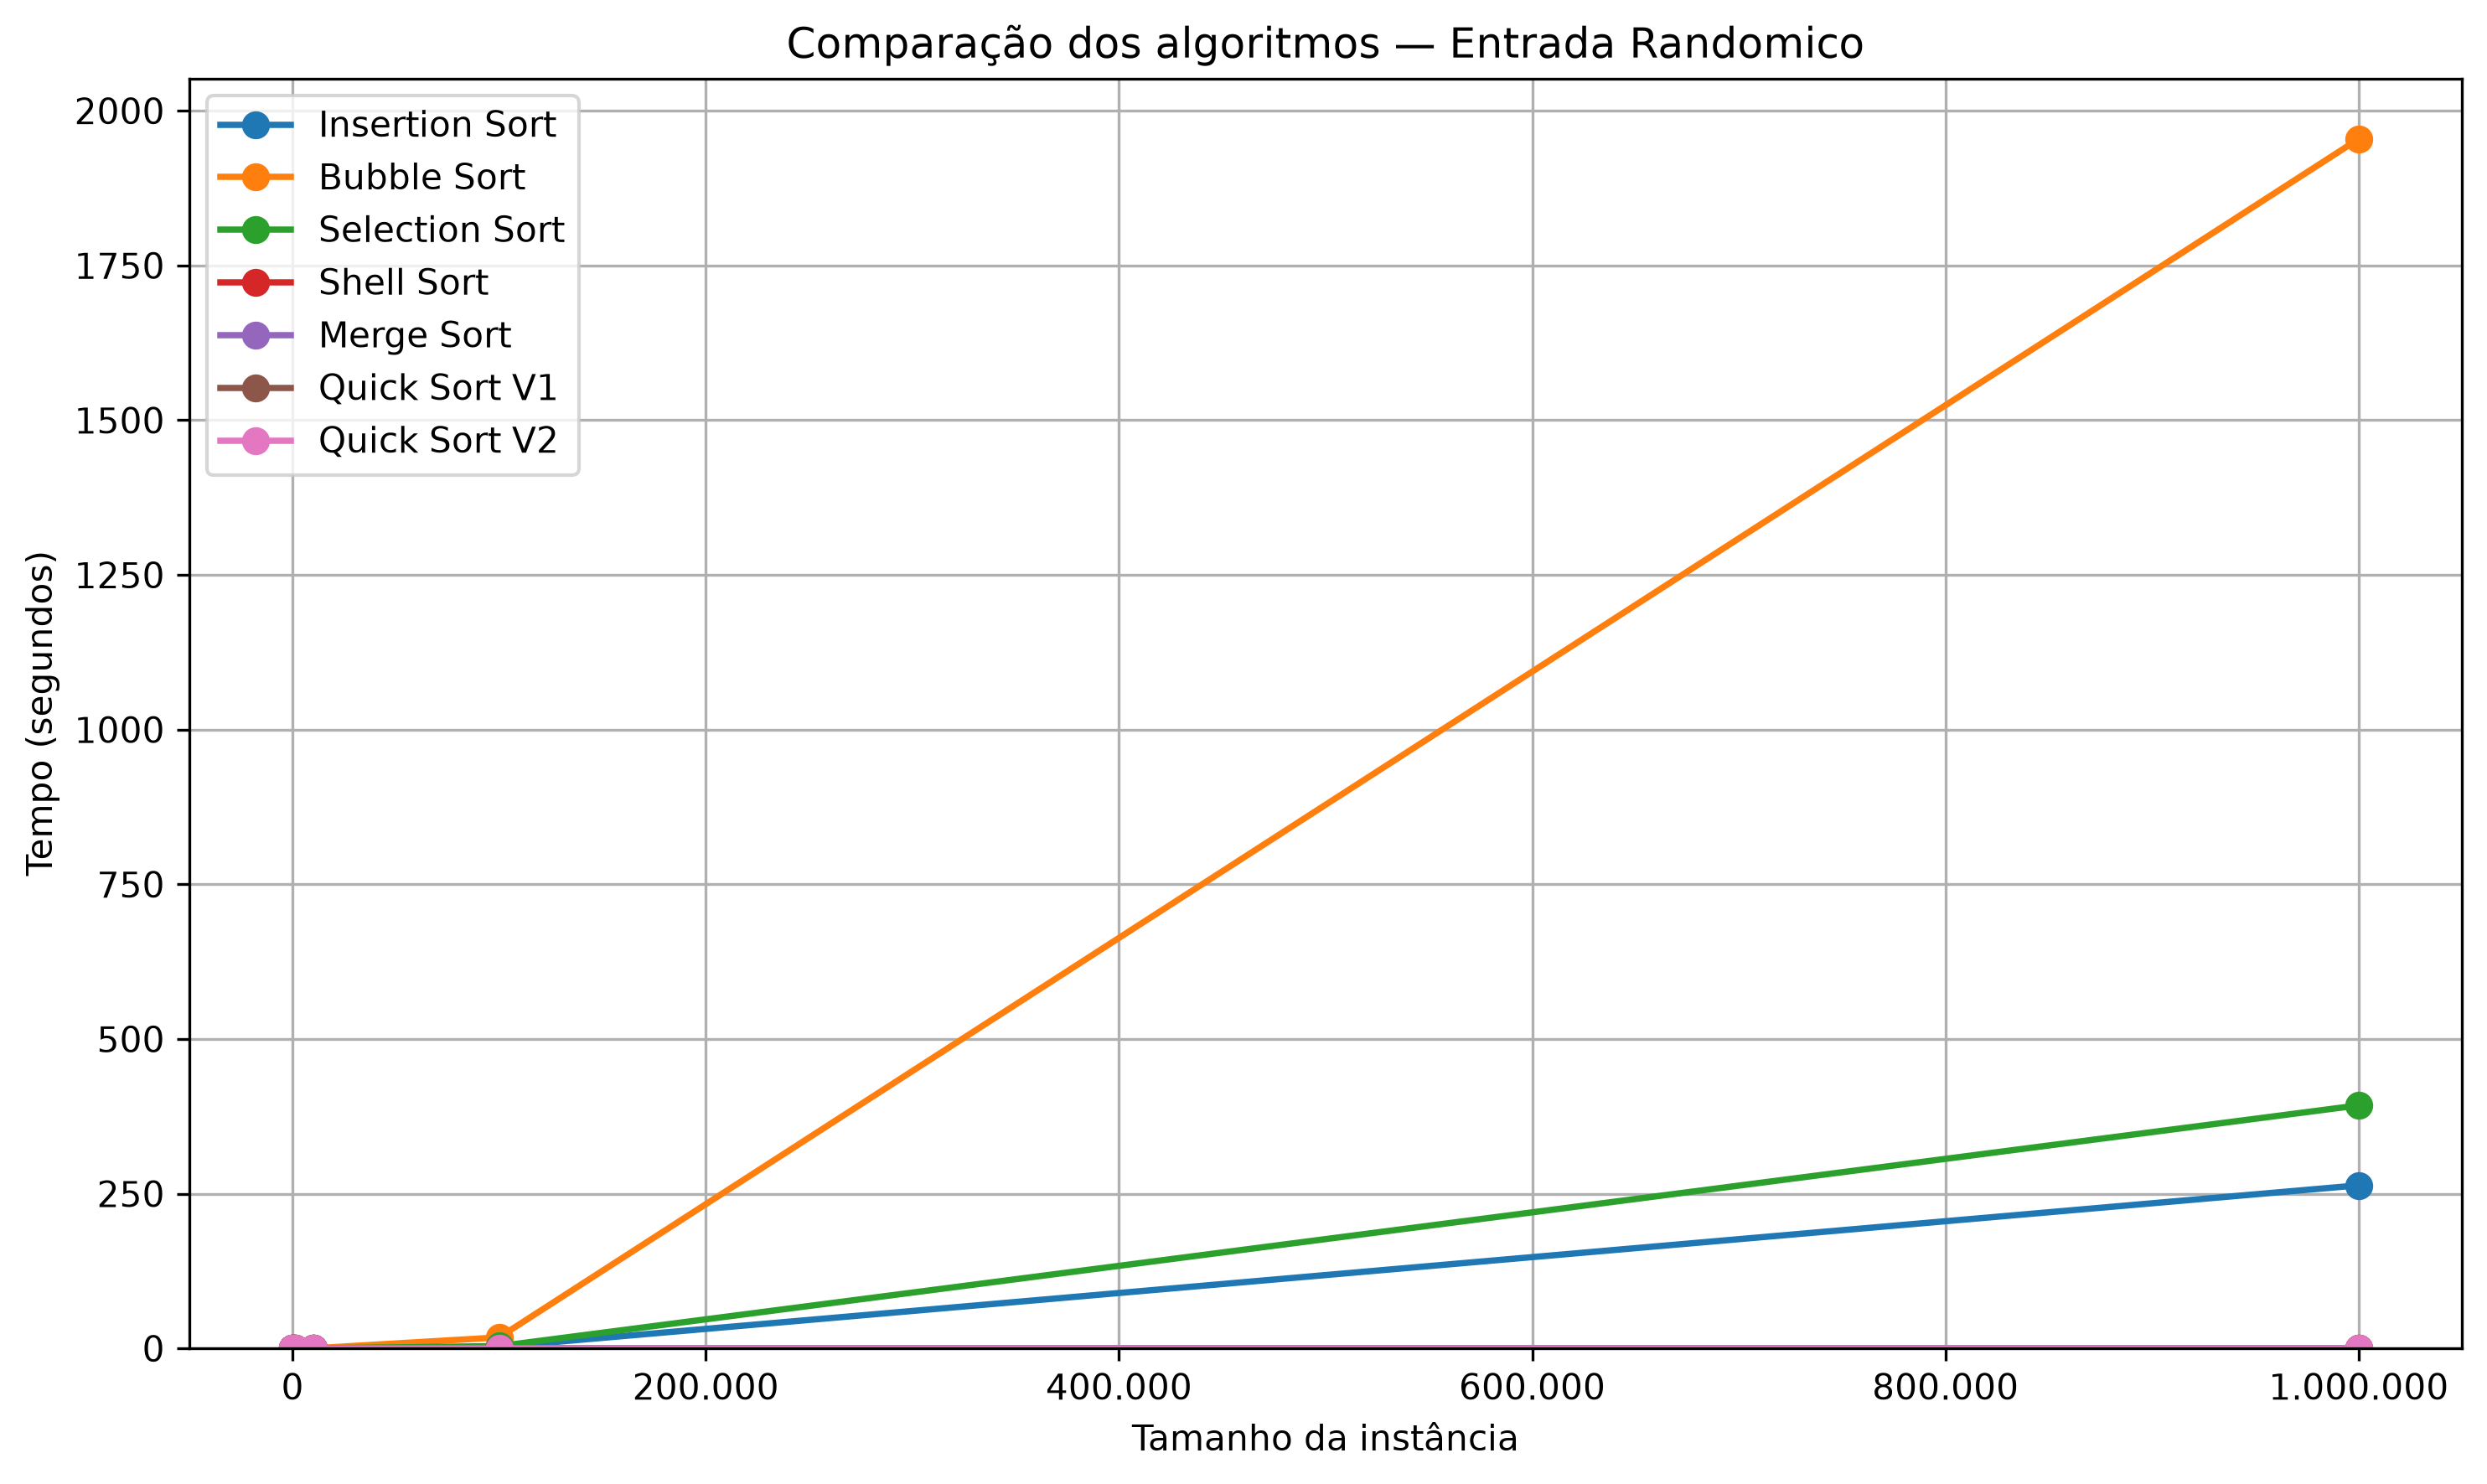
\includegraphics[width=\textwidth,keepaspectratio]{Imagens/Comparacoes/comparacao_aleatoria.png}
    \caption{Comparação dos algoritmos para entrada aleatória.}
    \label{fig:comparacao_aleatoria}
\end{figure}

Para as entradas aleatórias, observa-se uma separação clara entre os
algoritmos de custo quadrático e os demais. Para instâncias de
1.000.000 de elementos, o \textit{Bubble Sort} apresenta o maior tempo
de execução, em torno de 1950 segundos, seguido pelo \textit{Selection
Sort}, com cerca de 390 segundos, e pelo \textit{Insertion Sort}, com
cerca de 260 segundos. Esses resultados são coerentes com o crescimento
quadrático esperado no caso médio. A menor quantidade de deslocamentos do
\textit{Insertion Sort} em relação às trocas do \textit{Bubble Sort}
explica a diferença entre eles, mesmo com a mesma ordem de complexidade.

O \textit{Shell Sort}, o \textit{Merge Sort} e as duas versões do
\textit{Quick Sort} apresentaram tempos muito inferiores aos dos
algoritmos quadráticos, praticamente indistinguíveis do eixo horizontal
na escala do gráfico. Isso confirma, na prática, a vantagem dos
algoritmos com custo próximo de $\Theta(n\log n)$ para instâncias
grandes. No caso do \textit{Quick Sort}, as duas versões apresentaram
comportamento semelhante em entradas aleatórias, pois, nessa situação, o
primeiro elemento e a média aritmética tendem a gerar partições
razoavelmente equilibradas.


\newpage

% --------------------------------------------------
% ATIVIDADES MANUSCRITAS
% --------------------------------------------------

\section{ATIVIDADES MANUSCRITAS}
\subsection{Insertion Sort}

\begin{figure}[H]
\centering
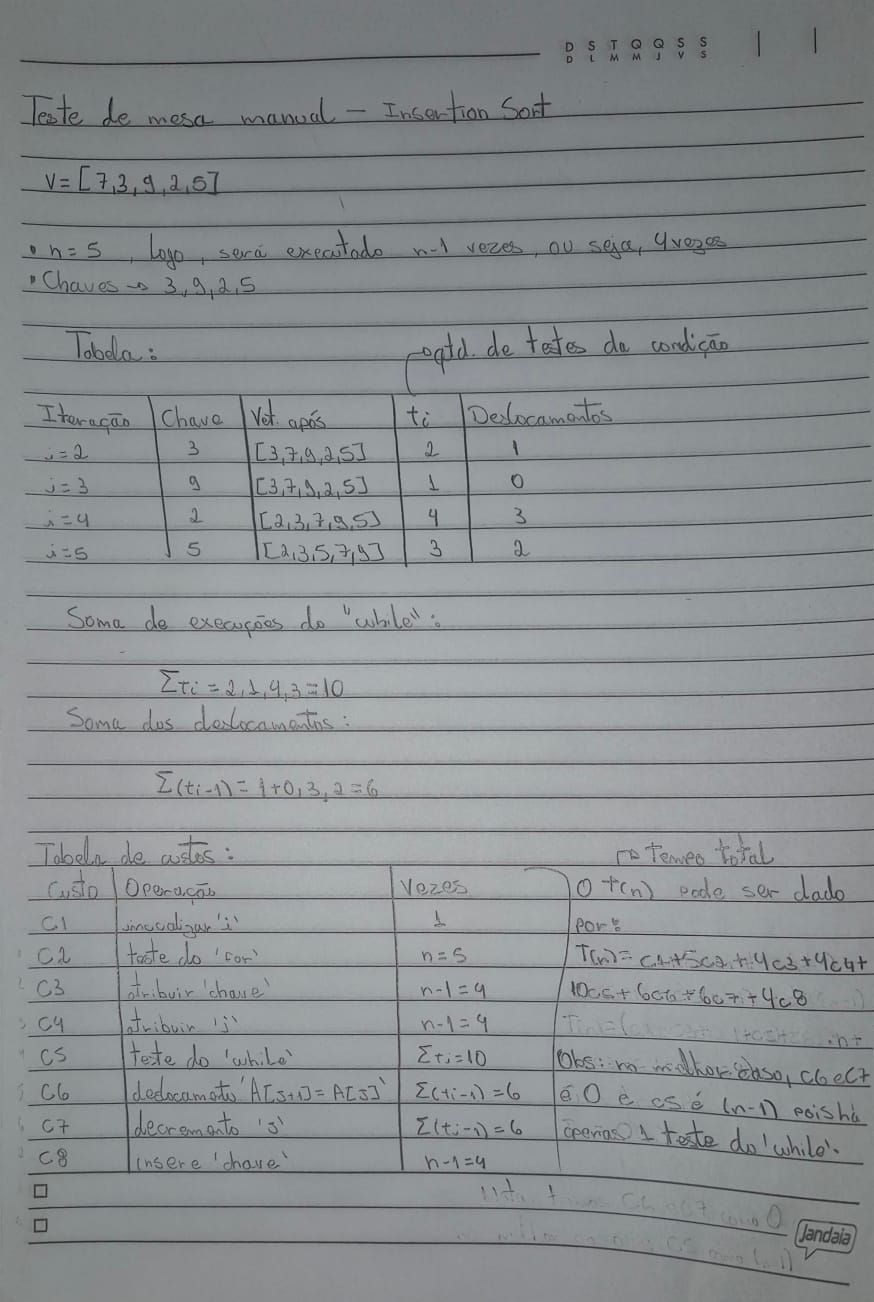
\includegraphics[width=13cm,keepaspectratio]{Imagens/Insertion_Sort/teste_mesa_insertionsort.jpeg}
\caption{Teste de mesa manual do algoritmo Insertion Sort}
\label{fig:teste-mesa-insertion}
\end{figure}

\begin{figure}[H]
\centering
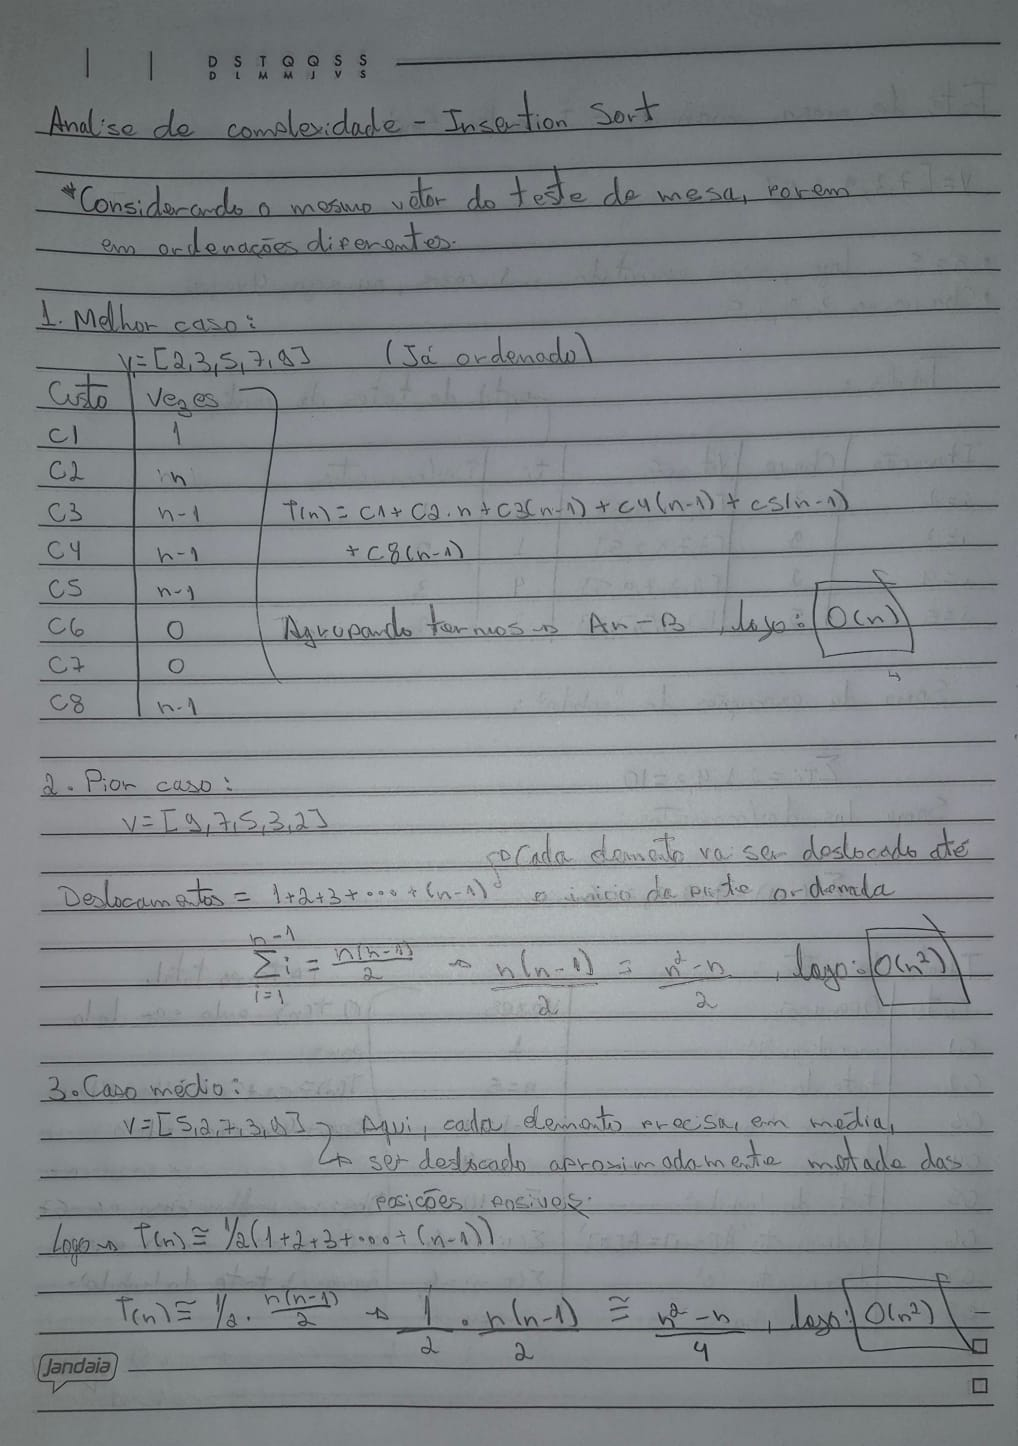
\includegraphics[width=13cm,keepaspectratio]{Imagens/Insertion_Sort/analise_complexidade_insertionsort.jpeg}
\caption{Análise de complexidade do algoritmo Insertion Sort}
\label{fig:analise-complexidade-insertion}
\end{figure}

\clearpage
\subsection{Bubble Sort}

\begin{figure}[H]
\centering
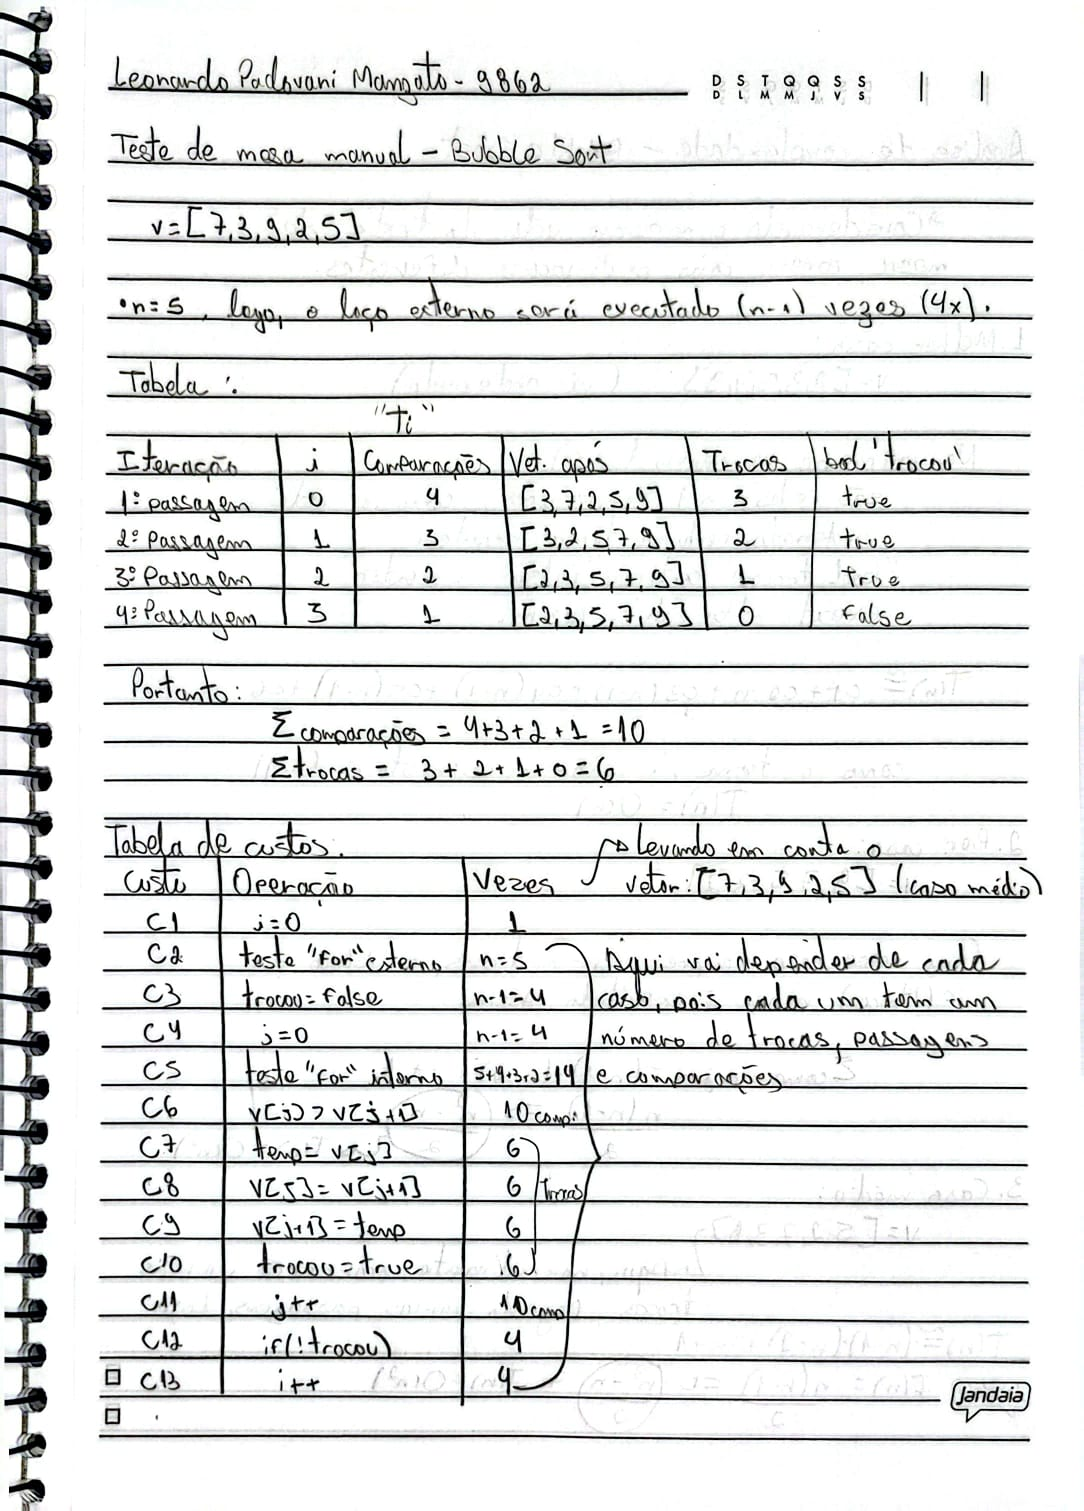
\includegraphics[width=13cm,keepaspectratio]{Imagens/Bubble_Sort/teste_mesa_bubblesort.jpeg}
\caption{Teste de mesa manual do algoritmo Bubble Sort}
\label{fig:teste-mesa-bubble}
\end{figure}

\begin{figure}[H]
\centering
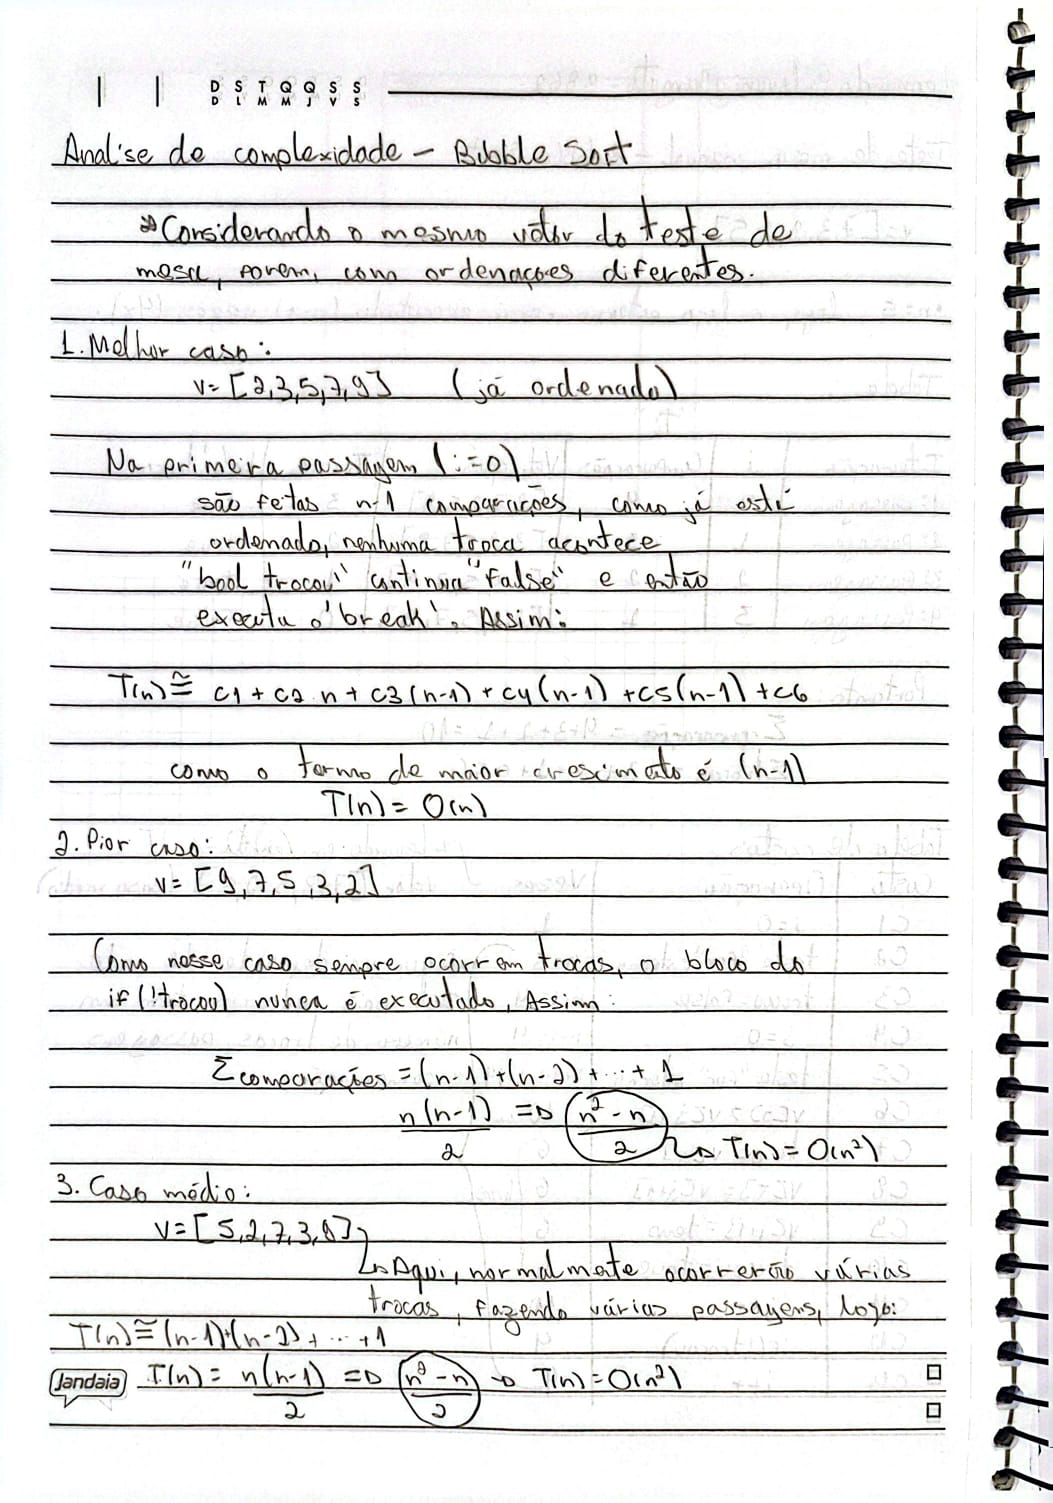
\includegraphics[width=13cm,keepaspectratio]{Imagens/Bubble_Sort/analise_complexidade_bubblesort.jpeg}
\caption{Análise de complexidade do algoritmo Bubble Sort}
\label{fig:analise-complexidade-bubble}
\end{figure}

\clearpage
\subsection{Selection Sort}

\begin{figure}[H]
\centering
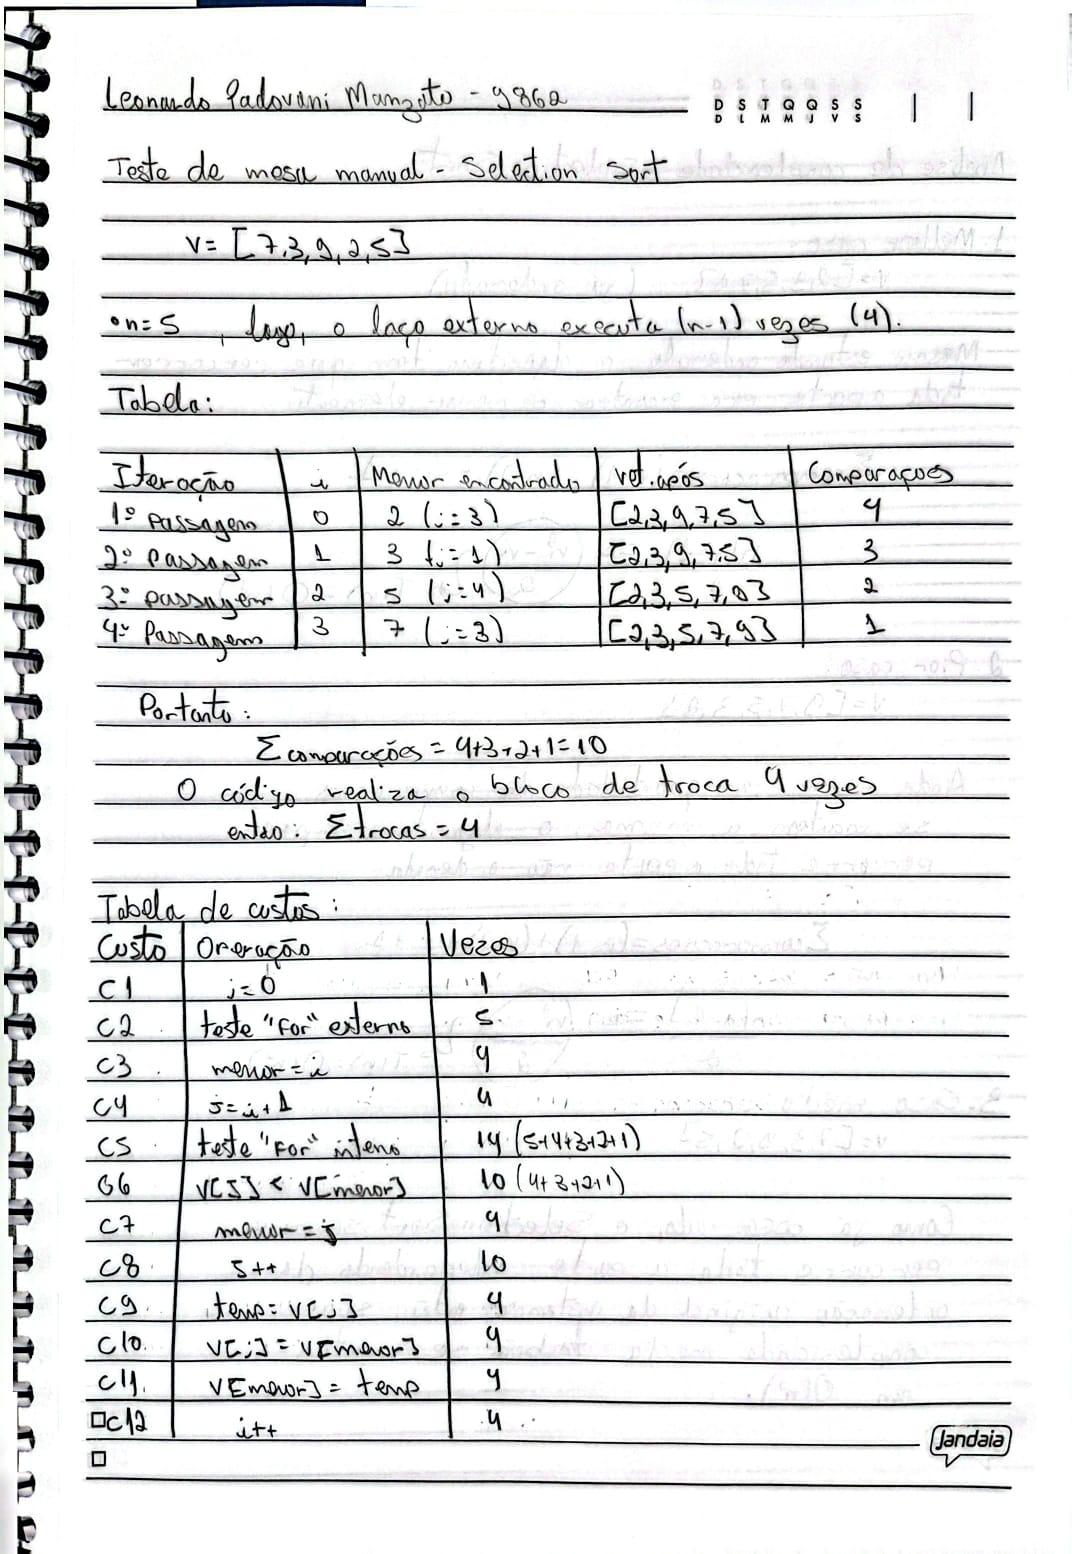
\includegraphics[width=13cm,keepaspectratio]{Imagens/Selection_Sort/teste_mesa_selectionsort.jpeg}
\caption{Teste de mesa manual do algoritmo Selection Sort}
\label{fig:teste-mesa-selection}
\end{figure}

\begin{figure}[H]
\centering
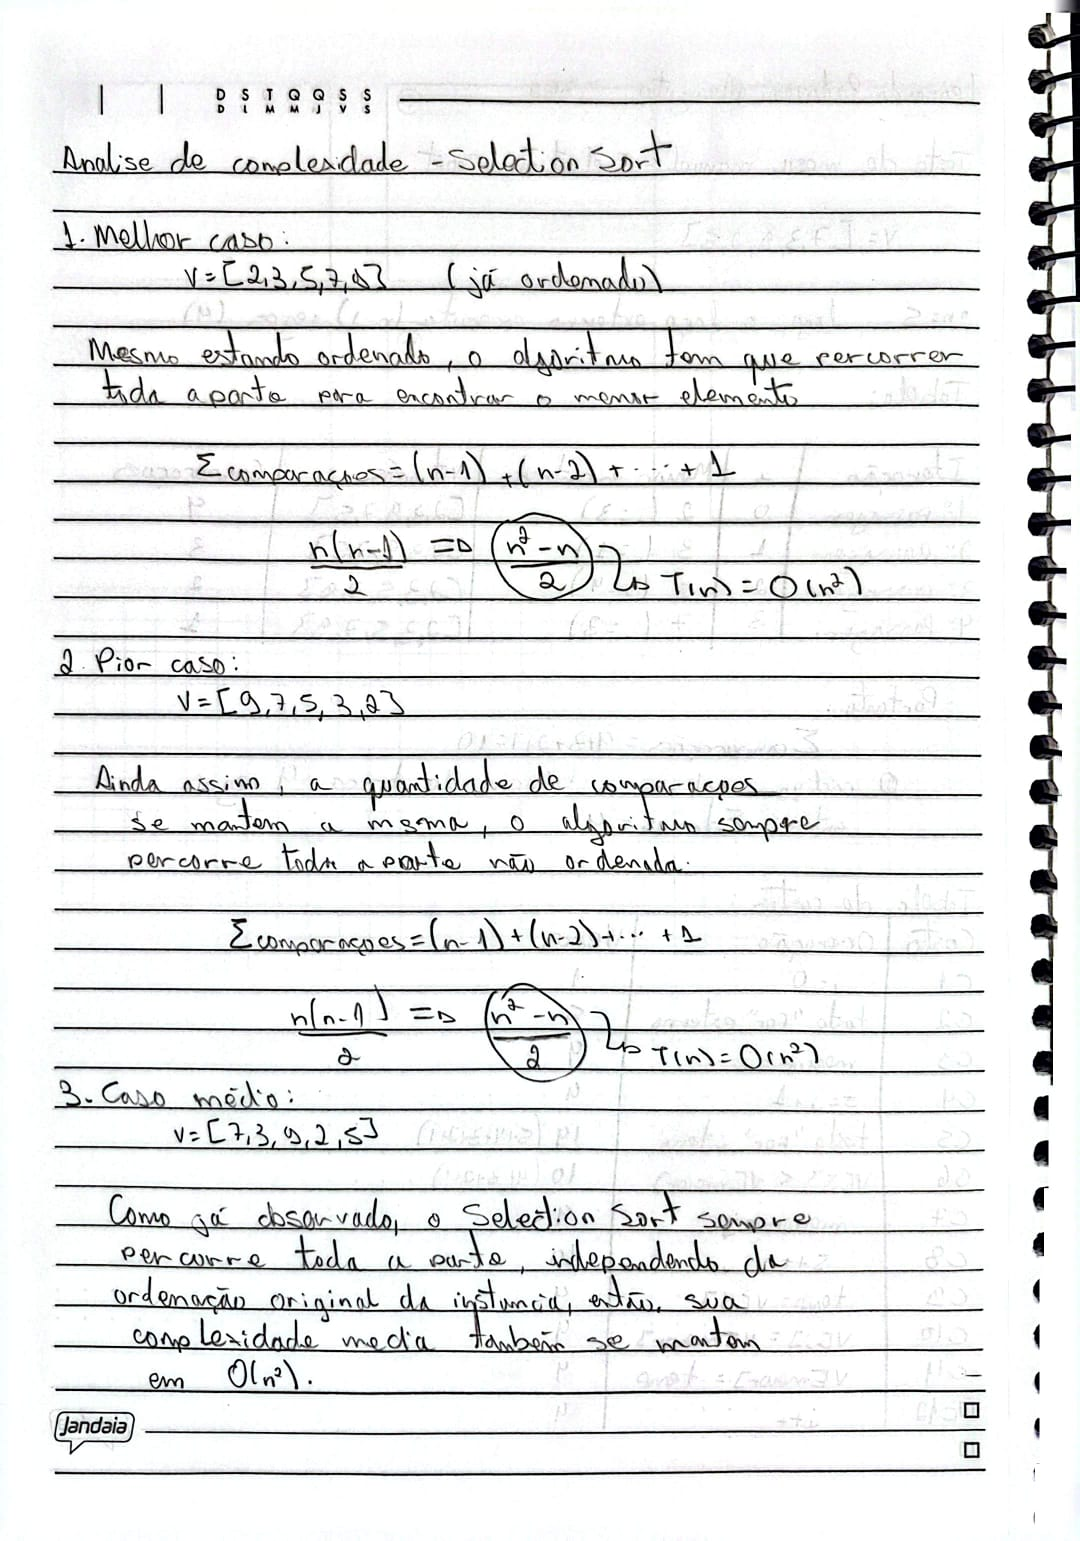
\includegraphics[width=13cm,keepaspectratio]{Imagens/Selection_Sort/analise_complexidade_selectionsort.jpeg}
\caption{Análise de complexidade do algoritmo Selection Sort}
\label{fig:analise-complexidade-selection}
\end{figure}

\clearpage
\subsection{Shell Sort}

\begin{figure}[H]
\centering
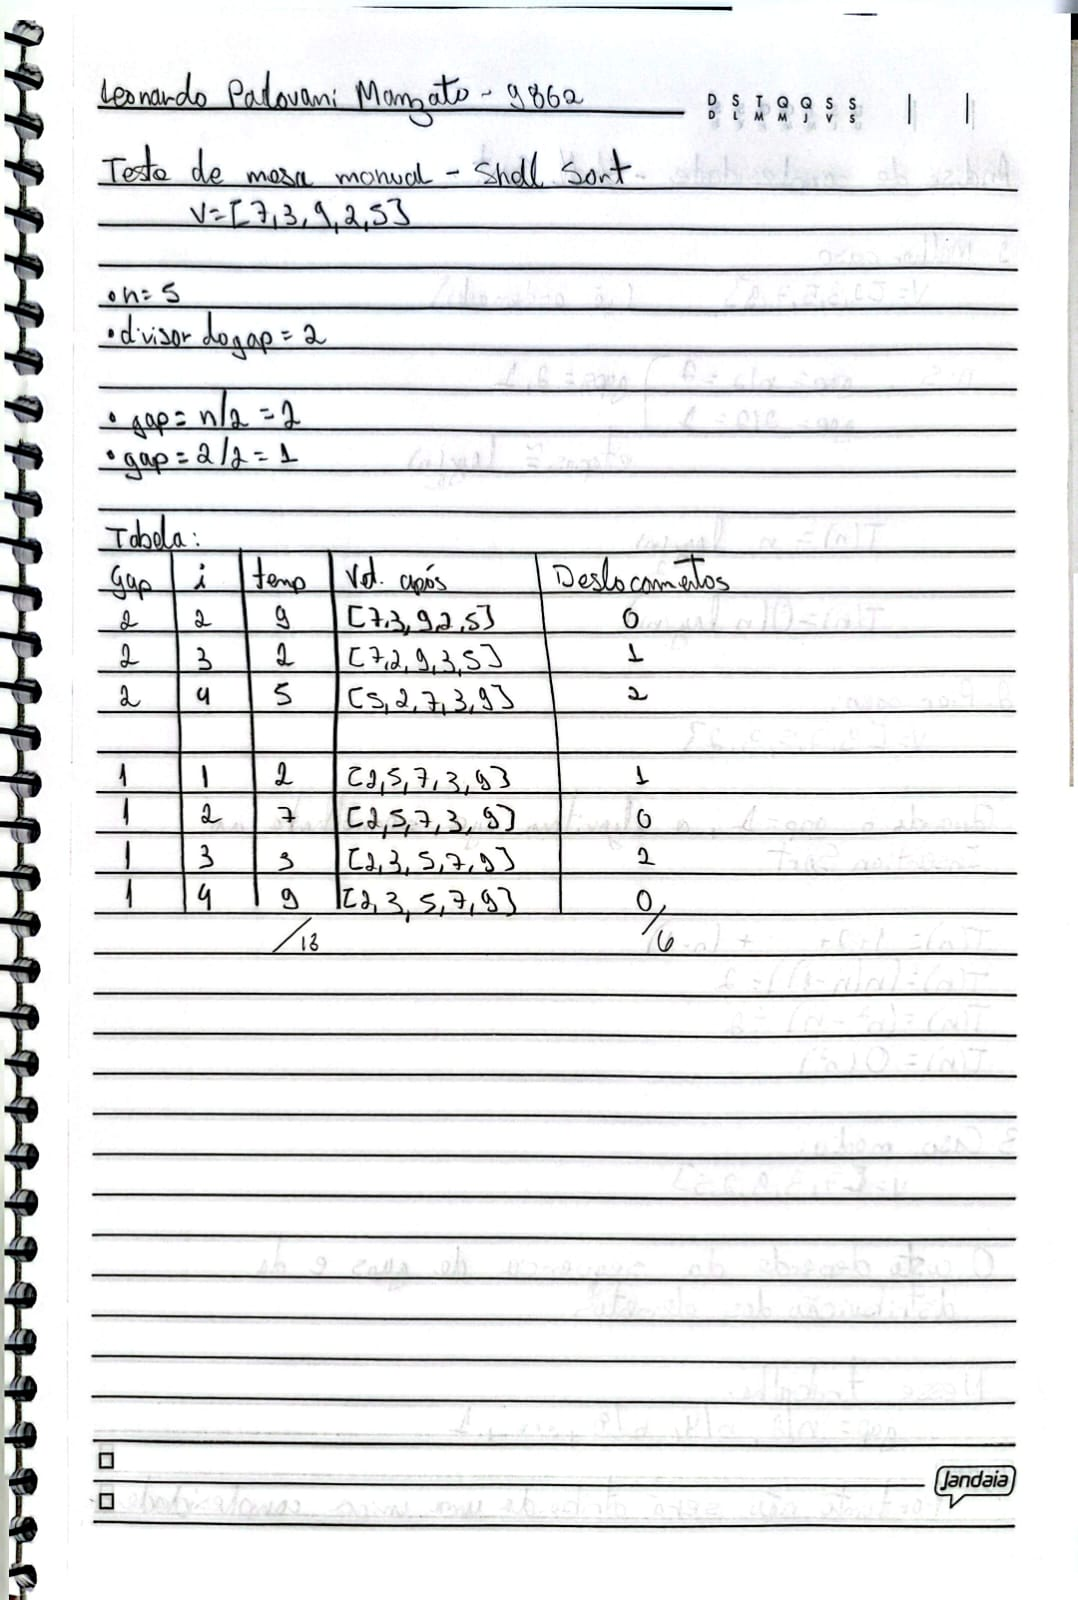
\includegraphics[width=13cm,keepaspectratio]
{Imagens/Shell_Sort/teste_mesa_shellsort.jpeg}
\caption{Teste de mesa manual do algoritmo Shell Sort}
\label{fig:teste-mesa-shell}
\end{figure}

\begin{figure}[H]
\centering
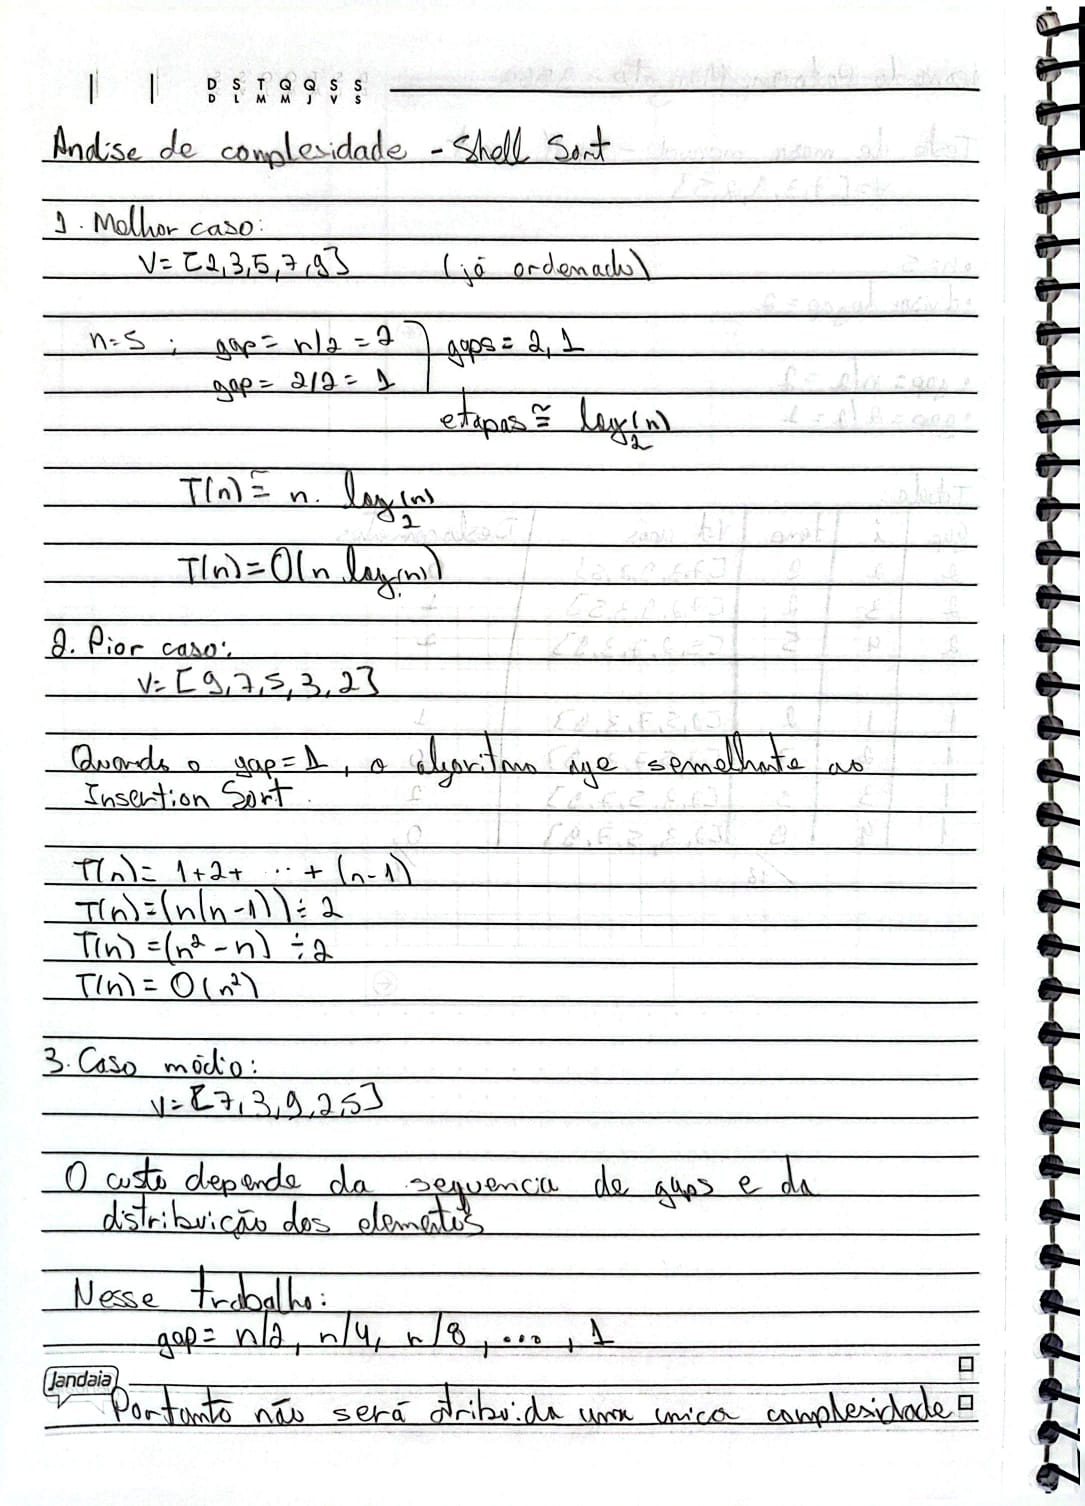
\includegraphics[width=13cm,keepaspectratio]{Imagens/Shell_Sort/analise_complexidade_shellsort.jpeg}
\caption{Análise de complexidade do algoritmo Shell Sort}
\label{fig:analise-complexidade-shell}
\end{figure}

\clearpage
\subsection{Merge Sort}

\begin{figure}[H]
\centering
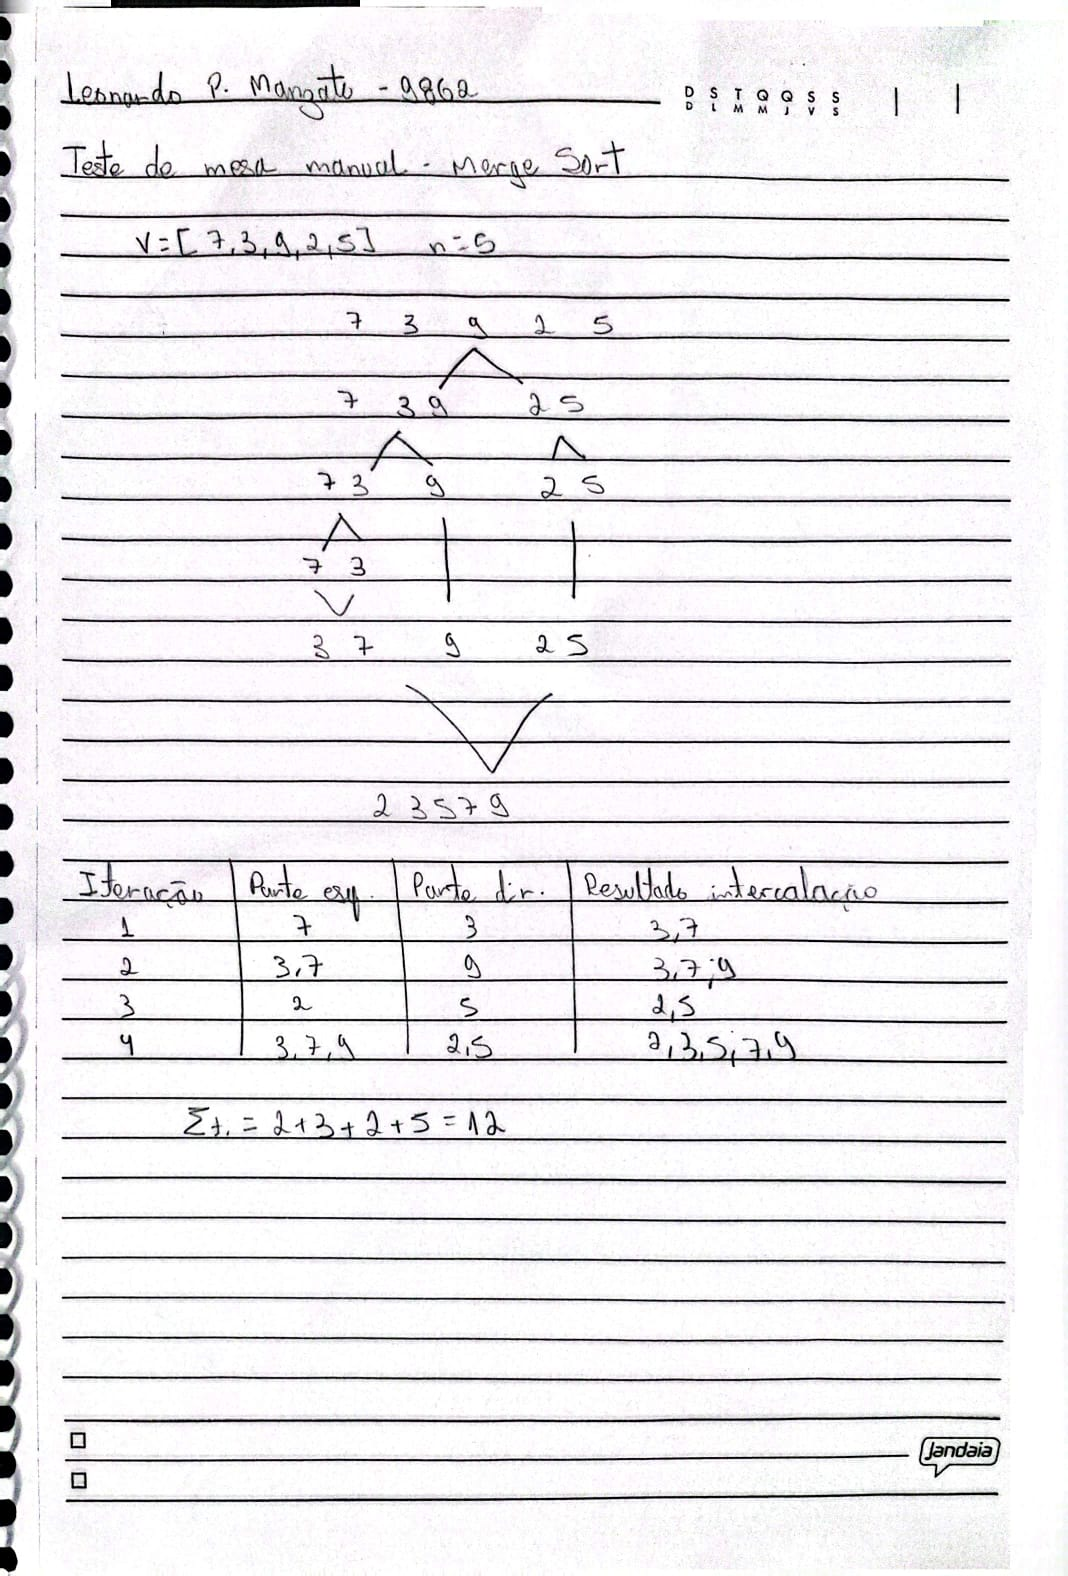
\includegraphics[width=13cm,keepaspectratio]
{Imagens/Merge_Sort/teste_mesa_mergesort.jpeg}
\caption{Teste de mesa manual do algoritmo Merge Sort}
\label{fig:teste-mesa-merge}
\end{figure}

\begin{figure}[H]
\centering
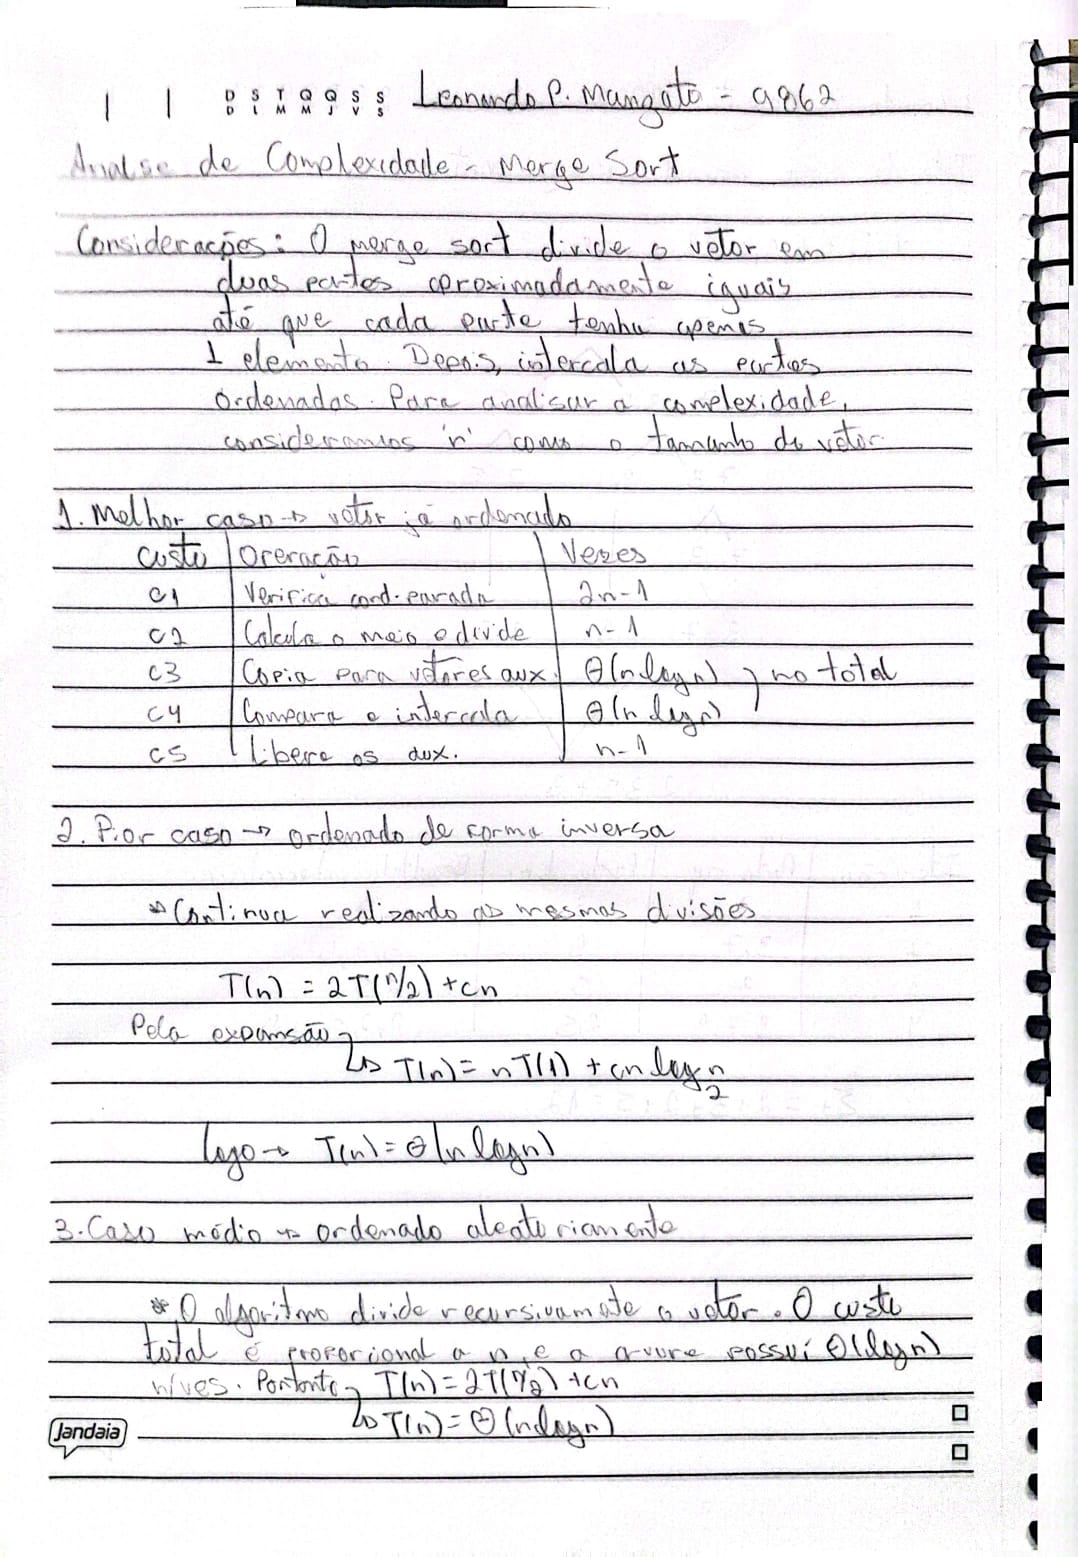
\includegraphics[width=13cm,keepaspectratio]{Imagens/Merge_Sort/analise_complexidade_mergesort.jpeg}
\caption{Análise de complexidade do algoritmo Merge Sort}
\label{fig:analise-complexidade-merge}
\end{figure}

\clearpage
\subsection{Quick Sort}

\subsubsection{Versão 1 (pivô no primeiro elemento)}

\begin{figure}[H]
\centering
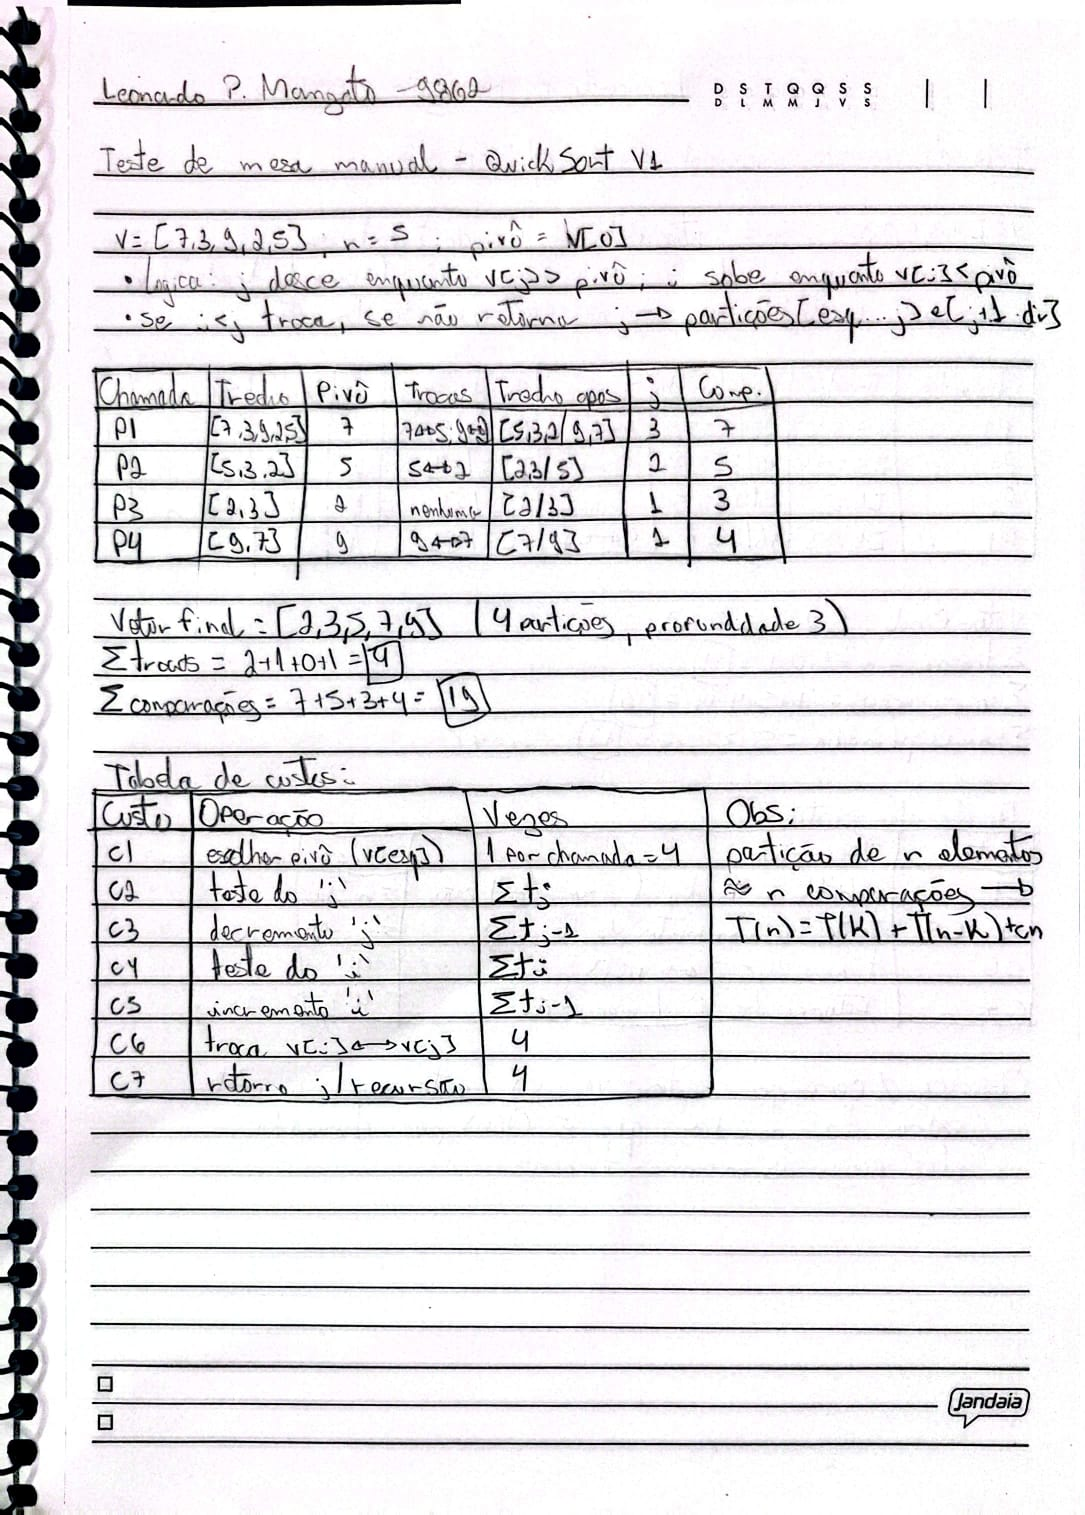
\includegraphics[width=13cm,keepaspectratio]{Imagens/Quick_Sort/teste_mesa_quicksort_v1.jpeg}
\caption{Teste de mesa manual do algoritmo Quick Sort (versão 1, pivô no primeiro elemento)}
\label{fig:teste-mesa-quick-v1}
\end{figure}

\begin{figure}[H]
\centering
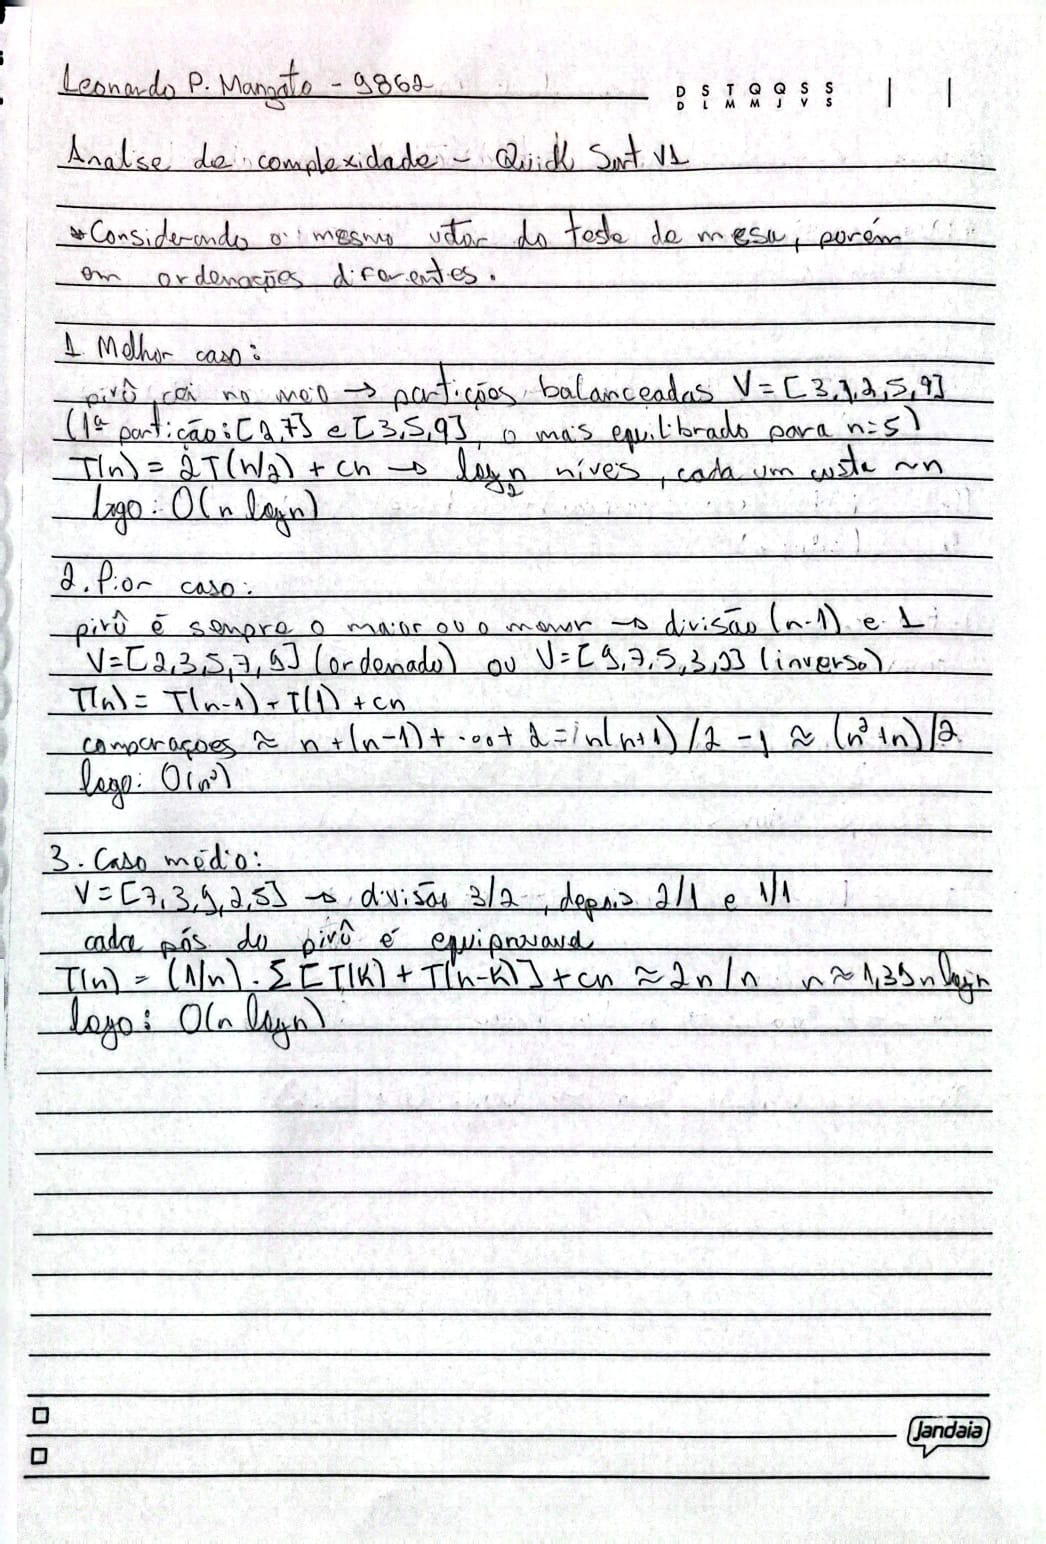
\includegraphics[width=13cm,keepaspectratio]{Imagens/Quick_Sort/analise_complexidade_quicksort_v1.jpeg}
\caption{Análise de complexidade do algoritmo Quick Sort (versão 1, pivô no primeiro elemento)}
\label{fig:analise-complexidade-quick-v1}
\end{figure}

\clearpage
\subsubsection{Versão 2 (pivô pela média aritmética)}

\begin{figure}[H]
\centering
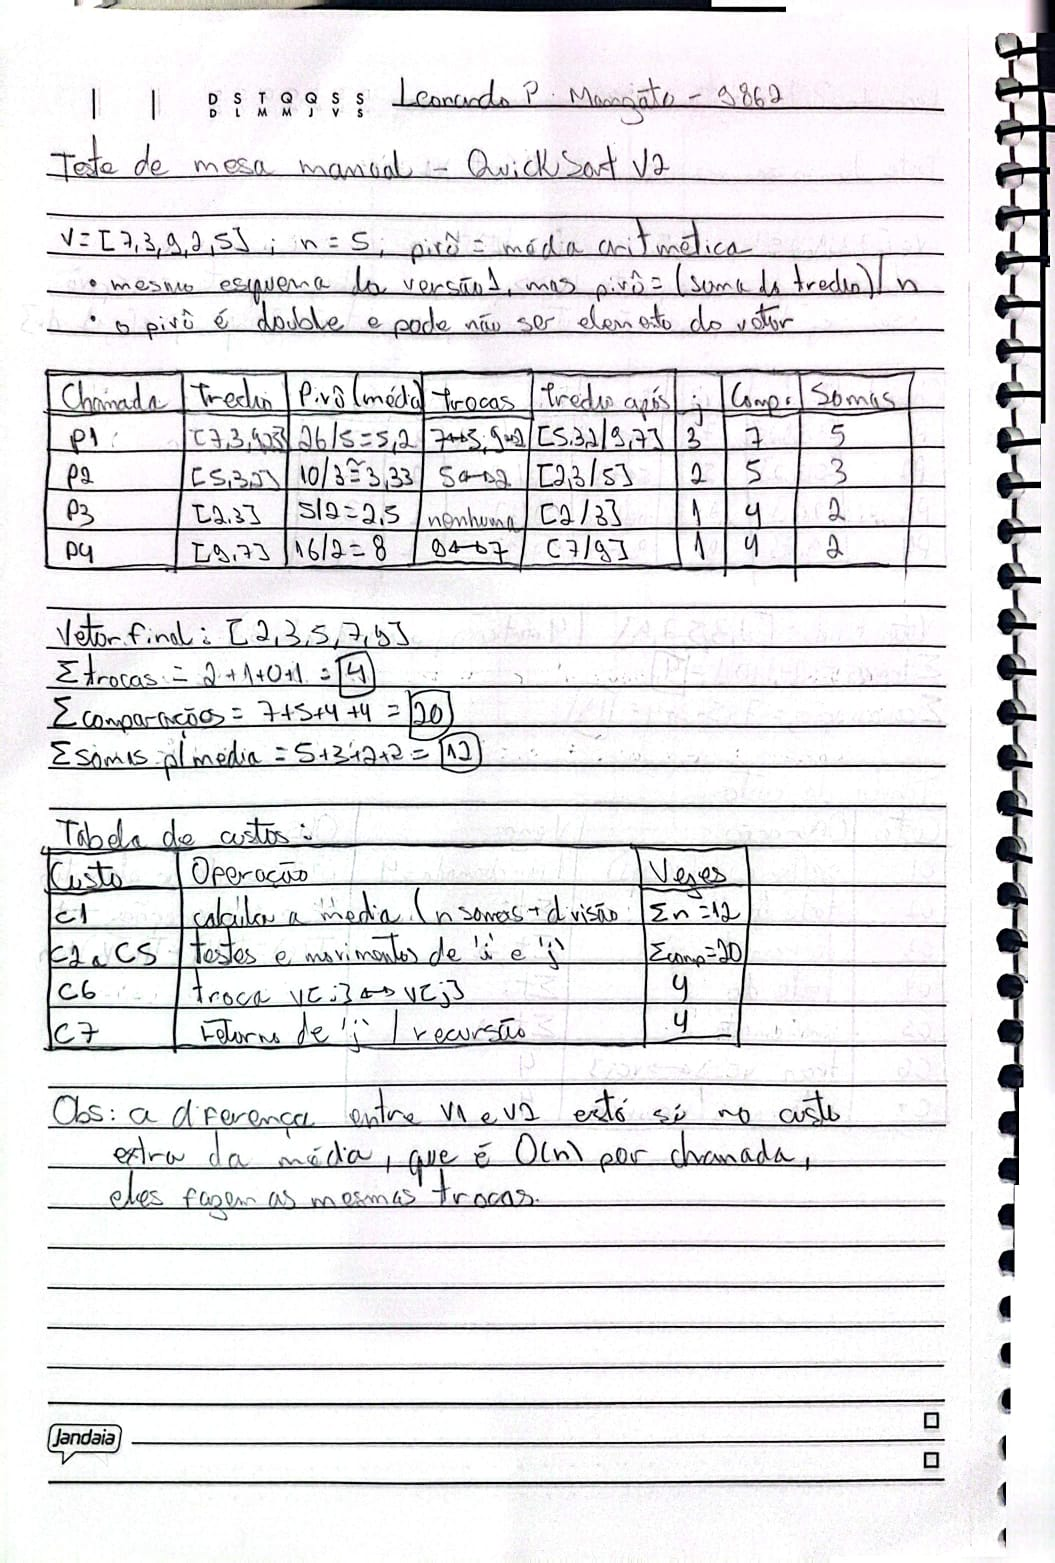
\includegraphics[width=13cm,keepaspectratio]{Imagens/Quick_Sort/teste_mesa_quicksort_v2.jpeg}
\caption{Teste de mesa manual do algoritmo Quick Sort (versão 2, pivô pela média aritmética)}
\label{fig:teste-mesa-quick-v2}
\end{figure}

\begin{figure}[H]
\centering
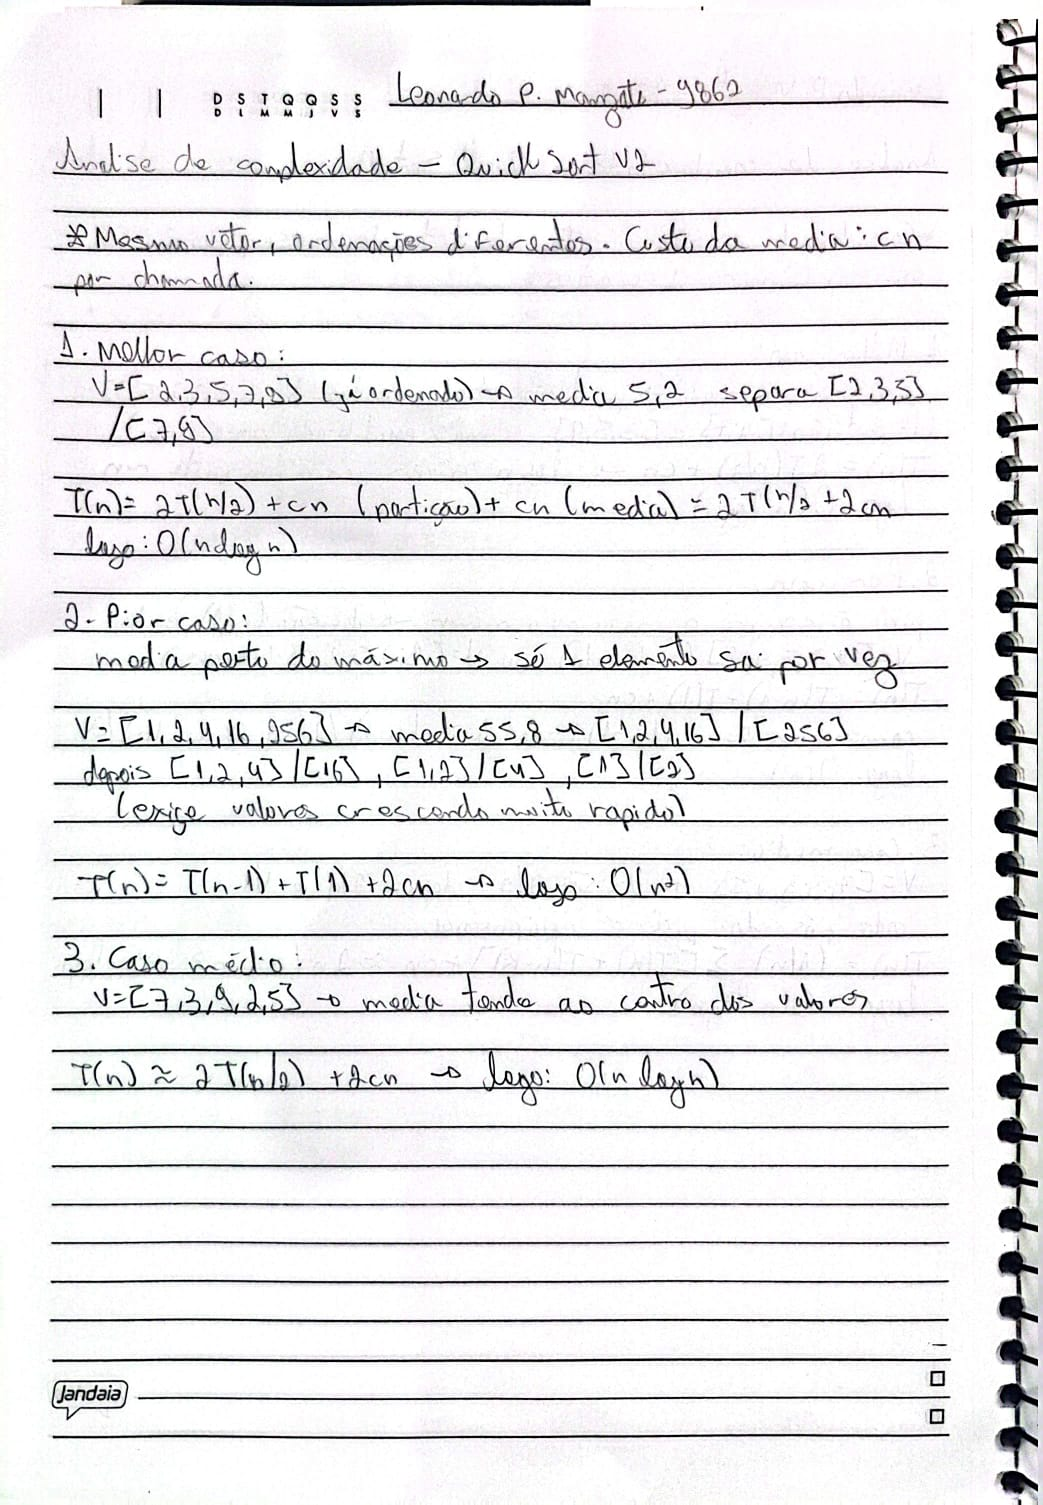
\includegraphics[width=13cm,keepaspectratio]{Imagens/Quick_Sort/analise_complexidade_quicksort_v2.jpeg}
\caption{Análise de complexidade do algoritmo Quick Sort (versão 2, pivô pela média aritmética)}
\label{fig:analise-complexidade-quick-v2}
\end{figure}

\newpage

% --------------------------------------------------
% CONCLUSÃO
% --------------------------------------------------

\section{CONCLUSÃO}
\quad A realização deste trabalho permitiu compreender o funcionamento dos
algoritmos \textit{Insertion Sort}, \textit{Bubble Sort}, \textit{Selection
Sort}, \textit{Shell Sort}, \textit{Merge Sort} e \textit{Quick Sort}, este
último em duas versões, além de analisar seus comportamentos em diferentes
tipos de entrada. Por meio das implementações, dos testes de mesa, das
análises de complexidade e dos experimentos práticos, foi possível observar
as diferenças entre as estratégias utilizadas por cada algoritmo.

\quad A análise teórica mostrou que o \textit{Insertion Sort} apresenta
complexidade $\Theta(n)$ no melhor caso, quando o vetor já está ordenado, e
$\Theta(n^2)$ no caso médio e no pior caso. O \textit{Bubble Sort} e o
\textit{Selection Sort}, considerando as implementações utilizadas neste
trabalho, apresentam complexidade $\Theta(n^2)$ nos três casos analisados.
Já o \textit{Shell Sort} possui comportamento dependente da sequência de
\textit{gaps} utilizada. Na implementação estudada, com a divisão sucessiva
do \textit{gap} por 2, o melhor caso apresenta crescimento de ordem
$\Theta(n\log n)$, enquanto o pior caso apresenta complexidade
$\Theta(n^2)$. O \textit{Merge Sort} apresenta complexidade temporal
$\Theta(n\log n)$ no melhor caso, no caso médio e no pior caso, além de
necessitar de memória auxiliar proporcional ao tamanho do vetor. Por fim, o
\textit{Quick Sort} apresenta complexidade $\Theta(n\log n)$ no melhor caso
e no caso médio, e $\Theta(n^2)$ no pior caso, que ocorre quando o pivô
gera partições muito desbalanceadas. Por ordenar o vetor no próprio local e
realizar a chamada recursiva apenas sobre a menor partição, a implementação
utilizada exige memória auxiliar de ordem $\Theta(\log n)$.

\quad Os experimentos realizados com entradas crescentes, decrescentes e
aleatórias permitiram observar na prática as diferenças previstas pela
análise teórica. No \textit{Insertion Sort}, a organização inicial dos
elementos possui influência significativa no tempo de execução: o tempo é
praticamente nulo quando o vetor já está ordenado e aproximadamente o dobro
do observado em entradas aleatórias quando ele está em ordem decrescente.
No \textit{Selection Sort}, o tempo foi semelhante nos três tipos de
entrada, pois a quantidade de comparações não depende da organização
inicial. O \textit{Bubble Sort} apresentou os maiores tempos em entradas
decrescentes e aleatórias, mas, devido à interrupção antecipada quando não
há trocas, teve tempo desprezível em entradas crescentes. O \textit{Shell
Sort} e o \textit{Merge Sort} apresentaram tempos muito inferiores aos dos
algoritmos quadráticos nos três tipos de entrada, o que evidencia a
vantagem dos algoritmos de custo próximo de $\Theta(n\log n)$ para
instâncias grandes.

\quad Os experimentos com o \textit{Quick Sort} evidenciaram a importância
da escolha do pivô. A versão 1, que utiliza o primeiro elemento, apresentou
tempos próximos aos dos algoritmos quadráticos em entradas crescentes e
decrescentes, pois nesses casos o pivô é sempre o menor ou o maior valor da
partição, levando o algoritmo ao pior caso. Em entradas aleatórias, porém,
seu tempo foi comparável ao dos algoritmos de custo $\Theta(n\log n)$. A
versão 2, que utiliza a média aritmética dos elementos como pivô, manteve
as partições equilibradas nos três tipos de entrada, com tempos muito
baixos, ao custo de um percurso adicional a cada particionamento. Vale
ressaltar que esse bom desempenho depende da distribuição dos valores
utilizados nos testes, pois a média aritmética pode gerar partições
desbalanceadas quando os valores são muito discrepantes.

\quad Também foi possível observar que o aumento do tamanho da entrada
provoca um crescimento no tempo de execução dos algoritmos. Esse
crescimento se torna mais significativo nos algoritmos e situações em que
há maior quantidade de comparações, trocas ou deslocamentos. Dessa forma,
os resultados experimentais possibilitam relacionar o comportamento
observado nos gráficos e tabelas com as complexidades obtidas na análise
teórica.

\quad No caso do \textit{Shell Sort}, teoricamente, a escolha do divisor
influencia a sequência de \textit{gaps} utilizada: um divisor menor produz
uma quantidade maior de etapas, enquanto um divisor maior reduz essa
quantidade. Entretanto, a quantidade de etapas, por si só, não determina o
tempo de execução, pois a sequência de \textit{gaps} também influencia a
quantidade de elementos que precisam ser comparados e deslocados. Como a
alteração do divisor não pôde ser implementada, os experimentos deste
trabalho utilizaram apenas o divisor 2, e a comparação entre diferentes
sequências de \textit{gaps} permanece como possibilidade de trabalho
futuro.

\quad Dessa forma, o trabalho permitiu relacionar conceitos teóricos de
análise de algoritmos com resultados obtidos por meio de experimentos
práticos. A comparação entre os seis algoritmos, considerando as duas
versões do \textit{Quick Sort}, mostrou que, apesar de todos possuírem o
mesmo objetivo de ordenar os elementos, suas estratégias de execução
produzem comportamentos diferentes de acordo com o tamanho e a organização
inicial da entrada. Os algoritmos de custo $\Theta(n\log n)$ se destacaram
em instâncias grandes, desde que, no caso do \textit{Quick Sort}, a escolha
do pivô evite partições desbalanceadas.

\newpage

% --------------------------------------------------
% REFERÊNCIAS
% --------------------------------------------------

\section{REFERÊNCIAS BIBLIOGRÁFICAS}
\begin{thebibliography}{99}

\bibitem{devfuria}
DEVFURIA.
\textit{Introdução ao algoritmo de ordenação Insertion Sort}.
Disponível em:
\url{http://devfuria.com.br/logica-de-programacao/introducao-ao-algoritmo-de-ordenacao-insertion-sort/}.
Acesso em: 14 set. 2026.

\bibitem{cplusplusrand}
CPLUSPLUS.COM.
\textit{rand -- C++ Reference}.
Disponível em:
\url{https://cplusplus.com/reference/cstdlib/rand/}.
Acesso em: 14 set. 2026.

\bibitem{guru99}
GURU99.
\textit{C++ Manipulação de arquivos: como abrir, gravar, ler e fechar arquivos em C++}.
Disponível em:
\url{https://www.guru99.com/pt/cpp-file-read-write-open.html}.
Acesso em: 14 set. 2026.

\bibitem{medirtempo}
NGHIATU.
\textit{8 maneiras de medir o tempo de execução em C / C++}.
Disponível em:
\url{https://ichi.nghiatu.com/pt/8-maneiras-de-medir-o-tempo-de-execucao-em-c-c-79591185633529}.
Acesso em: 14 set. 2026.

\bibitem{stackoverflowparametros}
STACK OVERFLOW EM PORTUGUÊS.
\textit{Como criar parâmetros opcionais em C++?}.
Disponível em:
\url{https://pt.stackoverflow.com/questions/514913/como-criar-par%c3%a2metros-opcionais-em-c}.
Acesso em: 27 set. 2026.

\bibitem{shellsort}
SCRIBD.
\textit{Método de Shell Sort Explicado}.
Disponível em:
\url{https://pt.scribd.com/document/945722840/Shell-Sort}.
Acesso em: 27 set. 2026.

\bibitem{bubblesort}
TRYBE.
\textit{Bubble Sort: o que é e como usar? Exemplos práticos!}.
Disponível em:
\url{https://blog.betrybe.com/tecnologia/bubble-sort-tudo-sobre/}.
Acesso em: 27 set. 2026.

\bibitem{selectionsort}
JOÃO ARTHUR BARBOSA MOURA.
\textit{Estruturas de Dados e Algoritmos}.
Disponível em:
\url{https://joaoarthurbm.github.io/eda/posts/selection-sort/}.
Acesso em: 27 set. 2026.

\bibitem{comparacaoalgoritmos}
GEEKSFORGEEKS.
\textit{Comparison among Bubble Sort, Selection Sort and Insertion Sort}.
Disponível em:
\url{https://www.geeksforgeeks.org/dsa/comparison-among-bubble-sort-selection-sort-and-insertion-sort/}.
Acesso em: 27 set. 2026.

\bibitem{selectionbubble}
EDUCBA.
\textit{Selection sort vs Bubble sort | Differences of Selection sort vs Bubble sort}.
Disponível em:
\url{https://www.educba.com/selection-sort-vs-bubble-sort/}.
Acesso em: 27 set. 2026.

\bibitem{stackoverflow}
STACK OVERFLOW EM PORTUGUÊS.
\textit{Como passar uma função como parâmetro em C?}.
Disponível em:
\url{https://pt.stackoverflow.com/questions/2983/como-passar-uma-fun%C3%A7%C3%A3o-como-par%C3%A2metro-em-c}.
Acesso em: 14 set. 2026.

\bibitem{visualgo}
VISUALGO.
\textit{Sorting}.
Disponível em:
\url{https://visualgo.net/en/sorting}.
Acesso em: 27 set. 2026.

\bibitem{programizsorting}
PROGRAMIZ.
\textit{Sorting Algorithms}.
Disponível em:
\url{https://www.programiz.com/dsa/sorting-algorithm}.
Acesso em: 27 set. 2026.

\bibitem{programizshell}
PROGRAMIZ.
\textit{Shell Sort}.
Disponível em:
\url{https://www.programiz.com/dsa/shell-sort}.
Acesso em: 27 set. 2026.

\bibitem{mergegiovani}
GIOVANI DA CRUZ.
\textit{Merge Sort: um método eficaz de ordenação}.
Disponível em:
\url{https://giovanidacruz.com.br/merge-sort-um-metodo-eficaz-de-ordenacao/}.
Acesso em: 24 out. 2026.

\bibitem{geeksmerge}
GEEKSFORGEEKS.
\textit{Merge Sort}.
Disponível em:
\url{https://www.geeksforgeeks.org/dsa/merge-sort/}.
Acesso em: 24 out. 2026.

\bibitem{coddymerge}
CODDY.
\textit{Merge Sort — Visualização de algoritmo de ordenação}.
Disponível em:
\url{https://coddy.tech/visualize/pt/sorting/merge-sort}.
Acesso em: 24 out. 2026.

\bibitem{geeksquick}
GEEKSFORGEEKS.
\textit{Quick Sort}.
Disponível em:
\url{https://www.geeksforgeeks.org/dsa/quick-sort-algorithm/}.
Acesso em: 9 nov. 2026.

\bibitem{imequick}
FEOFILOFF, Paulo.
\textit{Algoritmo Quicksort: análise da correção e do desempenho}.
Instituto de Matemática e Estatística, Universidade de São Paulo.
Disponível em:
\url{https://users.ime.usp.br/~pf/algoritmos/aulas/quick.html}.
Acesso em: 8 nov. 2026.

\bibitem{programizquick}
PROGRAMIZ.
\textit{QuickSort (With Code in Python/C++/Java/C)}.
Disponível em:
\url{https://www.programiz.com/dsa/quick-sort}.
Acesso em: 9 nov. 2026.

\bibitem{ia}
OPENAI.
\textit{ChatGPT}: ferramenta de inteligência artificial utilizada como
auxílio na elaboração e revisão dos scripts de geração de gráficos e tabelas e organização LaTex no OverLeaf na elaboração do relatório.
2026.


\end{thebibliography}

\newpage

% --------------------------------------------------
% FUNÇÕES
% --------------------------------------------------
\section{Funções}

\subsection{Calculo do tempo de execução}
\begin{lstlisting}[
    caption={Função utilizada para medir o tempo de execução},
    label={lst:calcular-tempo}
]
double calcularTempo(void (*algoritmo)(int*, int), int* vetor, int tamanho) {
    // salvar tempo do inicio
    auto inicio = chrono::steady_clock::now();

    // executar o algoritmo
    algoritmo(vetor, tamanho);

    // salvar o tempo do fim da execucao
    auto fim = chrono::steady_clock::now();

    // calcular duracao
    chrono::duration<double> tempo = fim - inicio;

    return tempo.count();
}
\end{lstlisting}

A função apresentada no Código~\ref{lst:calcular-tempo} é responsável por
medir o tempo de execução do algoritmo. Para isso, registra o instante
inicial, executa o algoritmo, registra o instante final e calcula a
diferença entre os dois instantes.

O valor retornado pela função representa o tempo de execução em segundos.

\newpage

\subsection{Execução dos algoritmos}
\begin{lstlisting}[
    caption={Função utilizada para executar os algoritmos de ordenação},
    label={lst:executar-algoritmo}
]
void executarAlgoritmo(function<void(int*, int)> algoritmo,
                            const string& nomeAlgoritmo,
                            const string& caminhoBase,
                            const string& caminhoCSV) {

    int tipo = escolherTipoInstancia();
    int tamanho = escolherTamanhoInstancia();

    cout << "\nGerando instancia...\n";
    int* vetor = gerarInstancia(tipo, tamanho);

    if (vetor == nullptr) {
        cout << "Erro ao gerar instancia.\n";
        return;
    }

    const string nomeInstancia = obterNomeInstancia(tipo);
    const string nomeArquivo =
        nomeInstancia + "_" + to_string(tamanho) + ".txt";

    const string caminhoEntradaBase =
        caminhoBase + "Arquivos de Entrada/";
    const string caminhoSaidaBase =
        caminhoBase + "Arquivos de Saida/";
    const string caminhoTempoBase =
        caminhoBase + "Arquivos de Tempo/";

    criarDiretorios(caminhoEntradaBase, caminhoSaidaBase,
                    caminhoTempoBase, nomeInstancia);

    const string caminhoEntrada =
        caminhoEntradaBase + nomeInstancia + "/" + nomeArquivo;
    const string caminhoSaida =
        caminhoSaidaBase + nomeInstancia + "/" + nomeArquivo;
    const string caminhoTempo =
        caminhoTempoBase + nomeInstancia + "/" + nomeArquivo;

    cout << "Salvando instancia de Arquivos de Entrada...\n";
    salvarVetor(caminhoEntrada, vetor, tamanho);

    cout << "Executando " << nomeAlgoritmo << "...\n";
    double tempo = calcularTempo(algoritmo, vetor, tamanho);

    cout << "Salvando instancia de Arquivos de Saida...\n";
    salvarVetor(caminhoSaida, vetor, tamanho);

    cout << "Salvando Arquivos de Tempo...\n";
    salvarTempo(caminhoTempo, tamanho, tempo);
    salvarCSV(caminhoCSV, tamanho, nomeInstancia, tempo);

    cout << "\n===== EXECUCAO CONCLUIDA =====\n";
    cout << "Algoritmo: " << nomeAlgoritmo << "\n";
    cout << "Tipo: " << nomeInstancia << "\n";
    cout << "Tamanho: " << tamanho << "\n";
    cout << "Tempo: " << tempo << " segundos\n";

    cout << "\nArquivos gerados:\n";
    cout << "Entrada: " << caminhoEntrada << "\n";
    cout << "Saida:   " << caminhoSaida << "\n";
    cout << "Tempo:   " << caminhoTempo << "\n";
    cout << "CSV:     " << caminhoCSV << "\n";

    delete[] vetor;
}
\end{lstlisting}

A função apresentada no Código~\ref{lst:executar-algoritmo} é responsável por coordenar a execução dos algoritmos de ordenação. Inicialmente, solicita ao usuário o tipo e o tamanho da instância e gera o vetor correspondente. Em seguida, define os caminhos dos arquivos e salva o vetor original no diretório de entrada.

Após essa etapa, a função executa o algoritmo recebido como parâmetro e mede seu tempo de execução por meio da função \texttt{calcularTempo}. Como o vetor é ordenado durante essa operação, seu conteúdo é salvo no diretório de saída. O tempo obtido também é armazenado em um arquivo individual e em um arquivo CSV, utilizado posteriormente para gerar tabelas e gráficos comparativos.

Por fim, são exibidas informações sobre a execução e os caminhos dos arquivos gerados. A memória alocada dinamicamente para armazenar o vetor é liberada com \texttt{delete[]}, evitando que essa alocação permaneça sem liberação.

\textbf{Observação sobre o uso de funções lambda:} Nas chamadas do Shell Sort, Merge Sort e do Quick Sort são utilizadas funções lambda para adaptar a chamada dos algoritmos à assinatura esperada pela função \texttt{executarAlgoritmo}, que recebe um ponteiro para função com dois parâmetros: o vetor e seu tamanho.

No Shell Sort, a função lambda permite passar o divisor do \textit{gap} como argumento adicional para \texttt{shellSort}. O exemplo a seguir mostra como capturar a variável \texttt{divisor} para utilizar o valor informado pelo usuário:

\begin{lstlisting}[
    caption={Chamada do Shell Sort utilizando uma função lambda},
    label={lst:lambda-shell}
]
executarAlgoritmo(
    [divisor](int* vetor, int tamanho) {
        shellSort(vetor, tamanho, divisor);
    },
    "Shell Sort",
    CAMINHO_SHELL,
    CSV_SHELL
);
\end{lstlisting}

Nesse exemplo, a captura \texttt{[divisor]} permite que a função lambda utilize o valor da variável externa \texttt{divisor}. É importante observar que, na implementação original, a chamada utiliza o valor fixo \texttt{2}. Para que o divisor informado pelo usuário seja utilizado, é necessário substituí-lo pela versão apresentada.

No Merge Sort, a função lambda permite chamar \texttt{mergeSort} passando apenas o vetor e seu tamanho, utilizando os valores padrão dos parâmetros \texttt{esq} e \texttt{dir}, conforme apresentado no exemplo a seguir:

\begin{lstlisting}[
    caption={Chamada do Merge Sort utilizando uma função lambda},
    label={lst:lambda-merge}
]
executarAlgoritmo(
    [](int* vetor, int tamanho) {
        mergeSort(vetor, tamanho);
    },
    "Merge Sort",
    CAMINHO_MERGE,
    CSV_MERGE
);
\end{lstlisting}

Nesse caso, os colchetes vazios \texttt{[]} indicam que a função lambda não precisa capturar variáveis externas. Ela recebe o vetor e seu tamanho e chama \texttt{mergeSort} com esses dois argumentos. Os parâmetros \texttt{esq} e \texttt{dir} assumem seus valores padrão, permitindo que a ordenação seja iniciada sobre o vetor inteiro.

Dessa forma, as funções lambda permitem que os dois algoritmos sejam executados pela mesma função \texttt{executarAlgoritmo}, mantendo a estrutura de geração das instâncias, medição do tempo e salvamento dos arquivos.

\end{document}
